\documentclass[10pt,a4paper]{report}
\usepackage[left=3.00cm, right=1.00cm, top=2.00cm, bottom=2.00cm, nohead, footskip=7mm]{geometry}
\usepackage[14pt]{extsizes}

\usepackage[utf8]{inputenc}
\usepackage[T1]{fontenc}
\usepackage{amsmath}
\usepackage{amsfonts}
\usepackage{amssymb}
\usepackage{pdfpages}
\usepackage{longtable}

\usepackage[russian]{babel}

% Ссылки внутри текста
\usepackage{hyperref}

% Отступ абзаца
\usepackage{indentfirst}
\setlength{\parindent}{1.5cm} 

% Межстрочный интервал
\usepackage{setspace}
\onehalfspacing % интервал 1.5

% Вставка изображений
\usepackage{graphicx}
\graphicspath{{../}}
\RequirePackage{caption}
\DeclareCaptionLabelSeparator{defffis}{ --- }
\captionsetup{justification=centering,labelsep=defffis}

% Настройка оглавлений
\usepackage{titlesec}
\newcommand{\hsp}{\hspace{20pt}}
\titleformat{\chapter}[hang]{\large\bfseries}{\thechapter{. }}{0pt}{\large\bfseries}
\titlelabel{hlabel-formati}
\titlespacing{\chapter}{42pt}{-80pt}{12pt}
\titleformat{\section}[hang]{\large\bfseries}{\thesection{. }}{0pt}{\large\bfseries}
\titlespacing{\section}{42pt}{12pt}{5pt plus 5pt}
\titleformat{\subsection}[hang]{\large\bfseries}{\thesubsection{. }}{0pt}{\large\bfseries}
\titlespacing{\subsection}{42pt}{12pt}{5pt plus 5pt}


% Настройка списков
\usepackage{enumitem}
\setlist{nolistsep, itemsep=0.3cm,parsep=0pt,leftmargin=1.9cm}

% Настройка листингов
\usepackage{listings}
\lstset{
	language = sql,
	extendedchars=\true,
	keepspaces=true,
	basicstyle=\scriptsize\sffamily,
	showstringspaces=\false,
	numbers=left,
	stepnumber=1,
	numbersep=5pt,
	frame=single,
	tabsize=2,
	captionpos=t,
	breaklines=true,
	breakatwhitespace=false,
	escapeinside={\#*}{*)}
}

% Cчётчик страниц, таблиц, иллюстраций, источников
\AtEndDocument{\label{lastpage}}
\AtEndDocument{
	\addtocounter{table}{-1}
	\refstepcounter{table}
	\label{lasttable}
%	\addtocounter{figure}{-1}
%	\refstepcounter{figure}
%	\lable{lastfigure}
}

\begin{document}
	\renewcommand\bibname{Список литературы}
	
	\includepdf[pages=1]{title.pdf}
	\includepdf[pages=1]{tech_task.pdf}
	
	\chapter*{Реферат}
	Курсовой проект заключается в реализации web-приложения для транспортной системы завода. В результате выполнения проекта было получено программное обеспечение предоставляющее возможность выполнять действия, необходимые для планирования и исполнения заказов доставки.

Приложение реализовано с использованием фреймворка Django на языке программирования Python 3. В качестве СУБД был использован PostgreSQL.

\textbf{Ключевые слова}: доставка, транспортная система, завод, web-приложение, PostgreSQL, Django.

РПЗ содержит \pageref{lastpage} страниц, 
10 таблиц,
20 иллюстраций,
7 ссылок на используемые источники.

	\newpage
	
	\tableofcontents
	\newpage

	\chapter*{Введение}
	\addcontentsline{toc}{chapter}{Введение}
	Одним из ключевых аспектов эффективного ведения любого крупного или среднего бизнеса в текущее время является хорошая связь между его сотрудниками. Быстрый и удобный доступ к данным позволяет оперативно координировать всех работников и минимизировать временные издержки по передаче актуальных задач. Поэтому, актуальным направлением в современном мире является разработка сервисов, реализующих данные возможности. Объектом разработки данного курсового проекта выбрана транспортная система завода, которая должна выполнять доставку заказов.

\textbf{Целью} данного курсовой работы является разработка базы данных для транспортной системы завода и web-приложения доступа к базе данных.

Выделены следующие задачи курсового проекта:
\begin{itemize}
	\item формализовать задание, определить необходимый функционал;
	\item для структурированного хранения информации спроектировать базу данных;
	\item проанализировать существующие СУБД и обосновать выбор одной из них;
	\item реализовать базу данных и интерфейс доступа к ней с использованием выбранной СУБД;
	\item обосновать выбор web-фреймворка;
	\item реализовать web-приложение для определённого функционала.
\end{itemize}

	\newpage

	\chapter{Аналитическая часть}
	\section{Постановка задачи}
Необходимо разработать базу данных, которая будет хранить информацию о сотрудниках, заказах, записях, дежурствах и о проездах машин через контрольно-пропускные пункты, а также web-приложение для предоставления этих данных.

Также должны быть реализованы различные категории сотрудников, для которых будет предоставляться определённый функционал по работе с данными транспортной системы. Для этого должна существовать возможность регистрации аккаунтов и дальнейшего взаимодействия с ними.

\newpage
\section{Формализация данных}
В соответствии с предметной областью, соответствующей описным набором требований, база данных должна хранить сущности, описанные ER-диаграммой на рисунке \ref{er_analitics}


\begin{figure}[ph!] 
	\begin{center}
%		{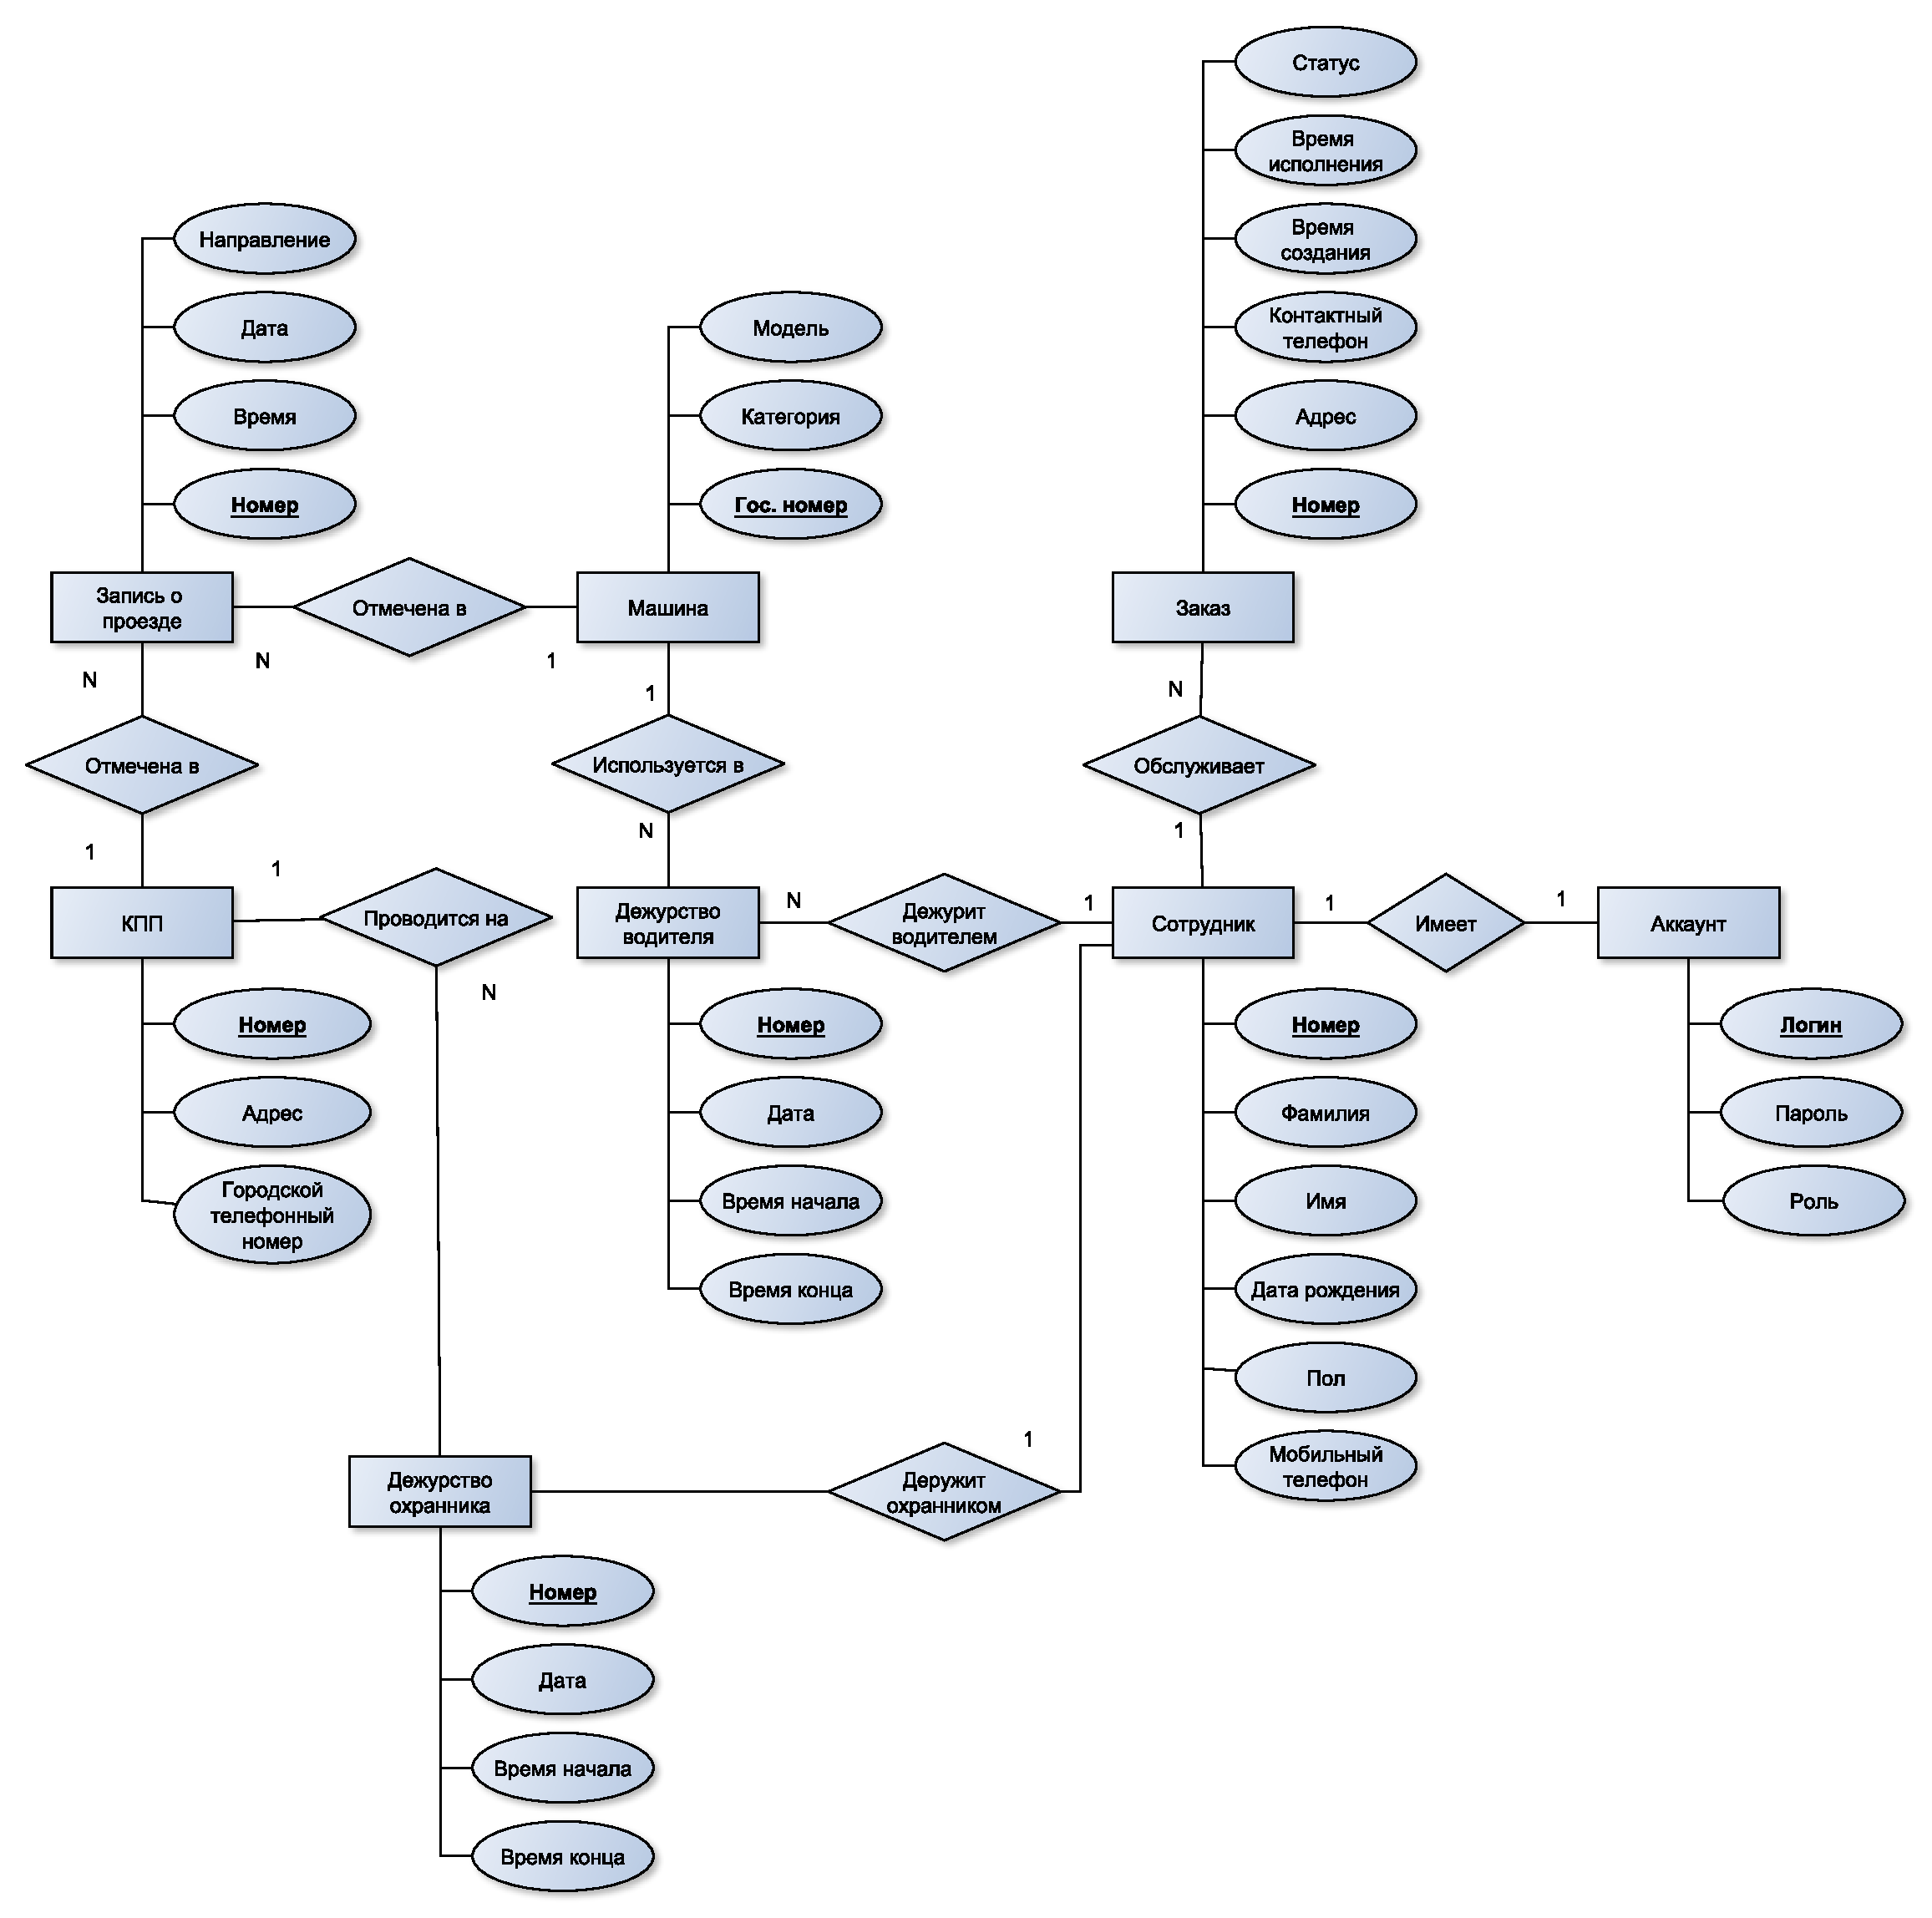
\includegraphics[height=18cm, width = 14cm]{schemes/er.pdf}}
		{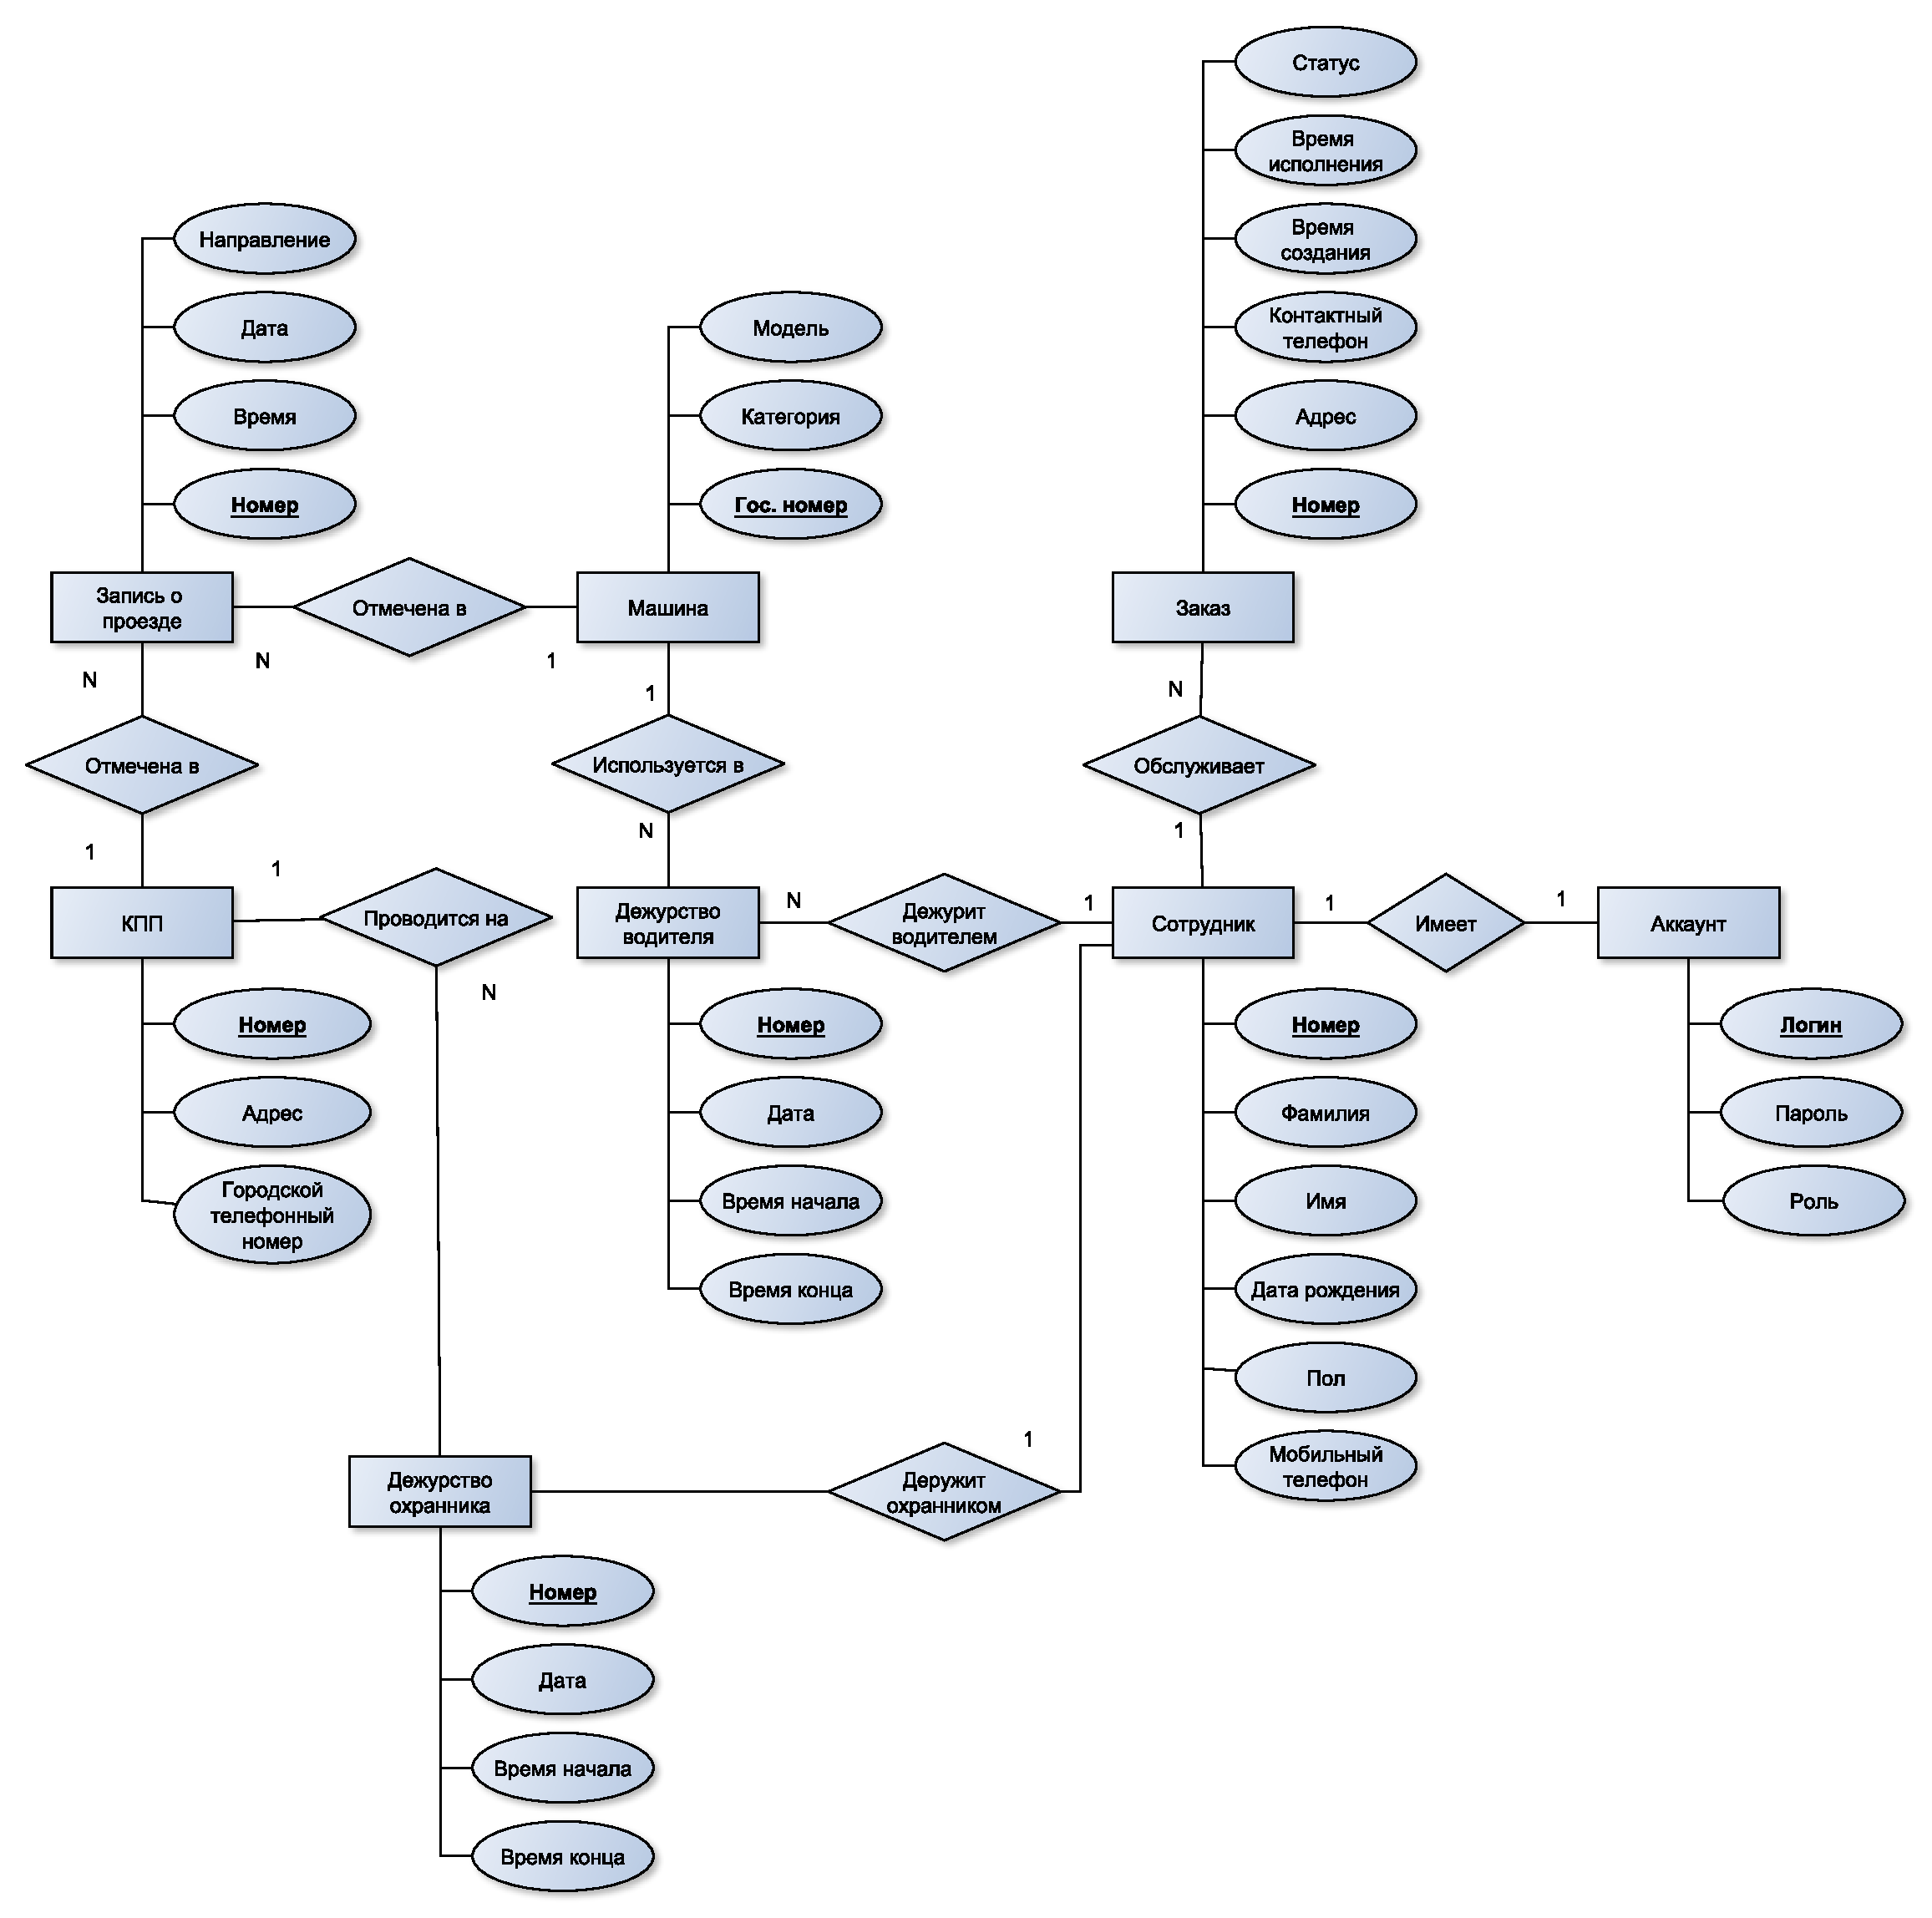
\includegraphics[scale=0.45]{schemes/er.pdf}}
		\caption{ER-диаграмма сущностей}
		\label{er_analitics}
	\end{center}
\end{figure}

\section{Формализация ролей}
Для функционирования транспортной системы были выделено несколько должностей сотрудников, названия и функционал которых приведены в таблице \ref{role_table}.

\begin{table}[h] 
	\caption{Роли сотрудников и их функционал}
	\label{role_table}
	\begin{tabular}{| p{4.5cm} | p{9.7cm} |}
		\hline
		\textbf{Должность}		&	\textbf{Функционал} \\
		\hline
		Администратор			&	
		Назначение дежурств и заказов, рассмотрение заявок на регистрацию, создание новых сущностей: машин, КПП, заказов  \\
		\hline
		
		Водитель &
		Выбор заказа, выполнение заказа, просмотр дежурств и личной информации \\
		\hline
		
		Охранник &
		Создание записей о проезде, просмотр дежурств и личной информации \\
		\hline
		
		Неподтверждённый сотрудник &
		Просмотр личной информации  \\	
		\hline	
		
		Неавторизованный пользователь &
		Регистрация, авторизация  \\		
		\hline
	\end{tabular}
\end{table}

Для упрощения регистрации новых сотрудников в системе принято решение предоставить им возможность заполнения заявок, которые в дальнейшем могут быть подтверждены администратором.

\section{Базы данных}
База данных — это совокупность взаимосвязанных структурированных данных, относящихся к определенной предметной области и организованных так, чтобы обеспечить независимость данных от программ обработки. \cite{db_model}

\subsection{Модели данных}
Модель данных - это абстрактное, самодостаточное, логическое определение объектов, операторов и прочих элементов, в совокупности составляющих абстрактную машину доступа к данным, с которой взаимодействует пользователь. Эти объекты позволяют моделировать
структуру данных, а операторы — поведение данных.
\cite{db_model2}

Существует три основные модели данных.
\begin{itemize}
	\item Иерархическая. База данных представляется в виде древовидной структуры, состоящей из объектов различных уровней. Объекты находятся в отношении предка к потомку, причём объект может иметь только одного предка и любое количество потомков.
	\item Сетевая. Отличием от иерархической модели данных является отсутствие ограничения на количество предков. База данных в такой модели состоит из набора экземпляров записи и экземпляров связей между записями.
	\item Реляционная. Основной идеей является то, что все наборы данных представляются в виде множеств. База данных состоит из множества двумерных таблиц. Таблицы состоят из записей и полей, каждая запись имеет собственные значения для каждого поля. Иерархия элементов отсутствует. 
\end{itemize}

Реляционная модель в настоящее время является наиболее гибкой и удобной в использовании, а также обладает наибольшим выбором в области систем управления базой данных, поэтому принято решение о её использовании в данной работе.


\subsection{СУБД}
Система управления базами данных (сокращённо СУБД) — совокупность
программных и лингвистических средств общего или специального назначения,
обеспечивающих управление созданием и использованием баз данных \cite{db_model}.

В процессе разработки было принято решение использовать СУБД для взаимодействия с базой данных, так как оно реализует множество функций, которые потребуются в работе с базой данных.


\section*{Вывод}
Результатом аналитического раздела стала постановка задачи, формализация данных программы и ролей пользователей, описание способов хранения данных и управления ими.

	\newpage
	
	\chapter{Конструкторская часть}
	\section{Диаграмма вариантов использования}
На рисунке \ref{use_case} представленна Use Case диаграмма сценариев использования с описанными ранее видами акторов.


\begin{figure}[ph!]
	\begin{center}
%		{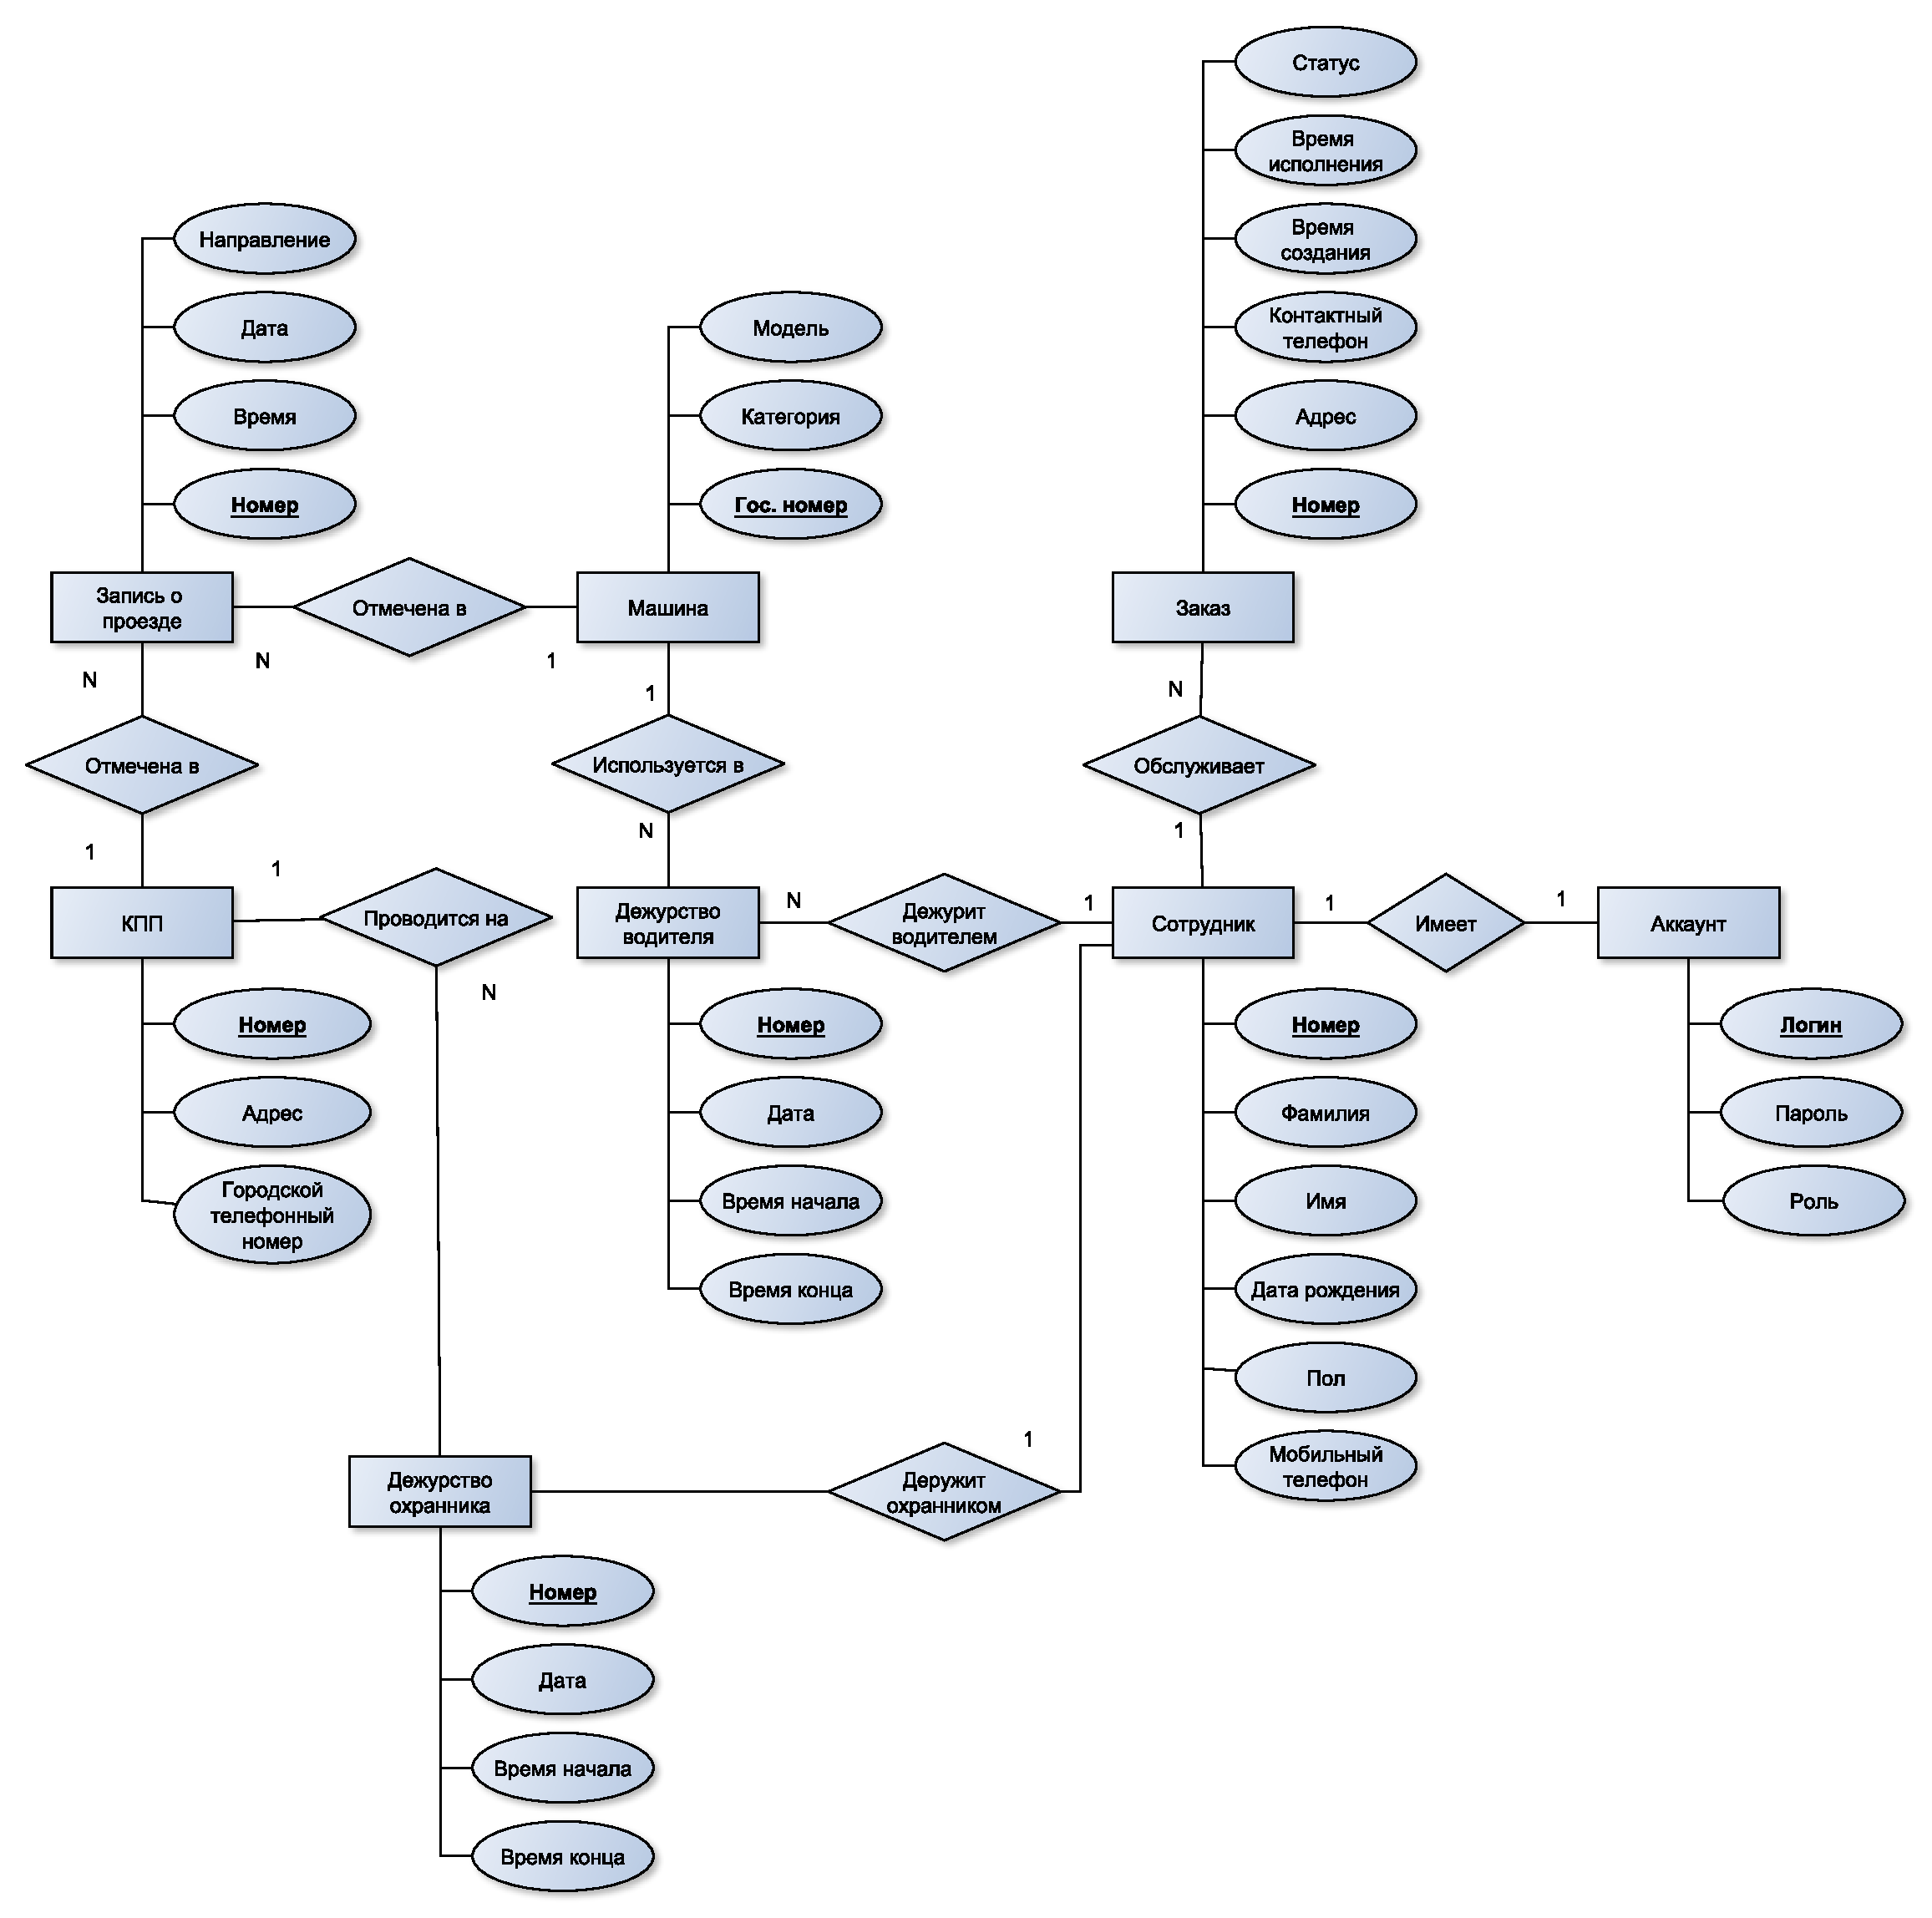
\includegraphics[height=18cm, width = 14cm]{schemes/er.pdf}}
		{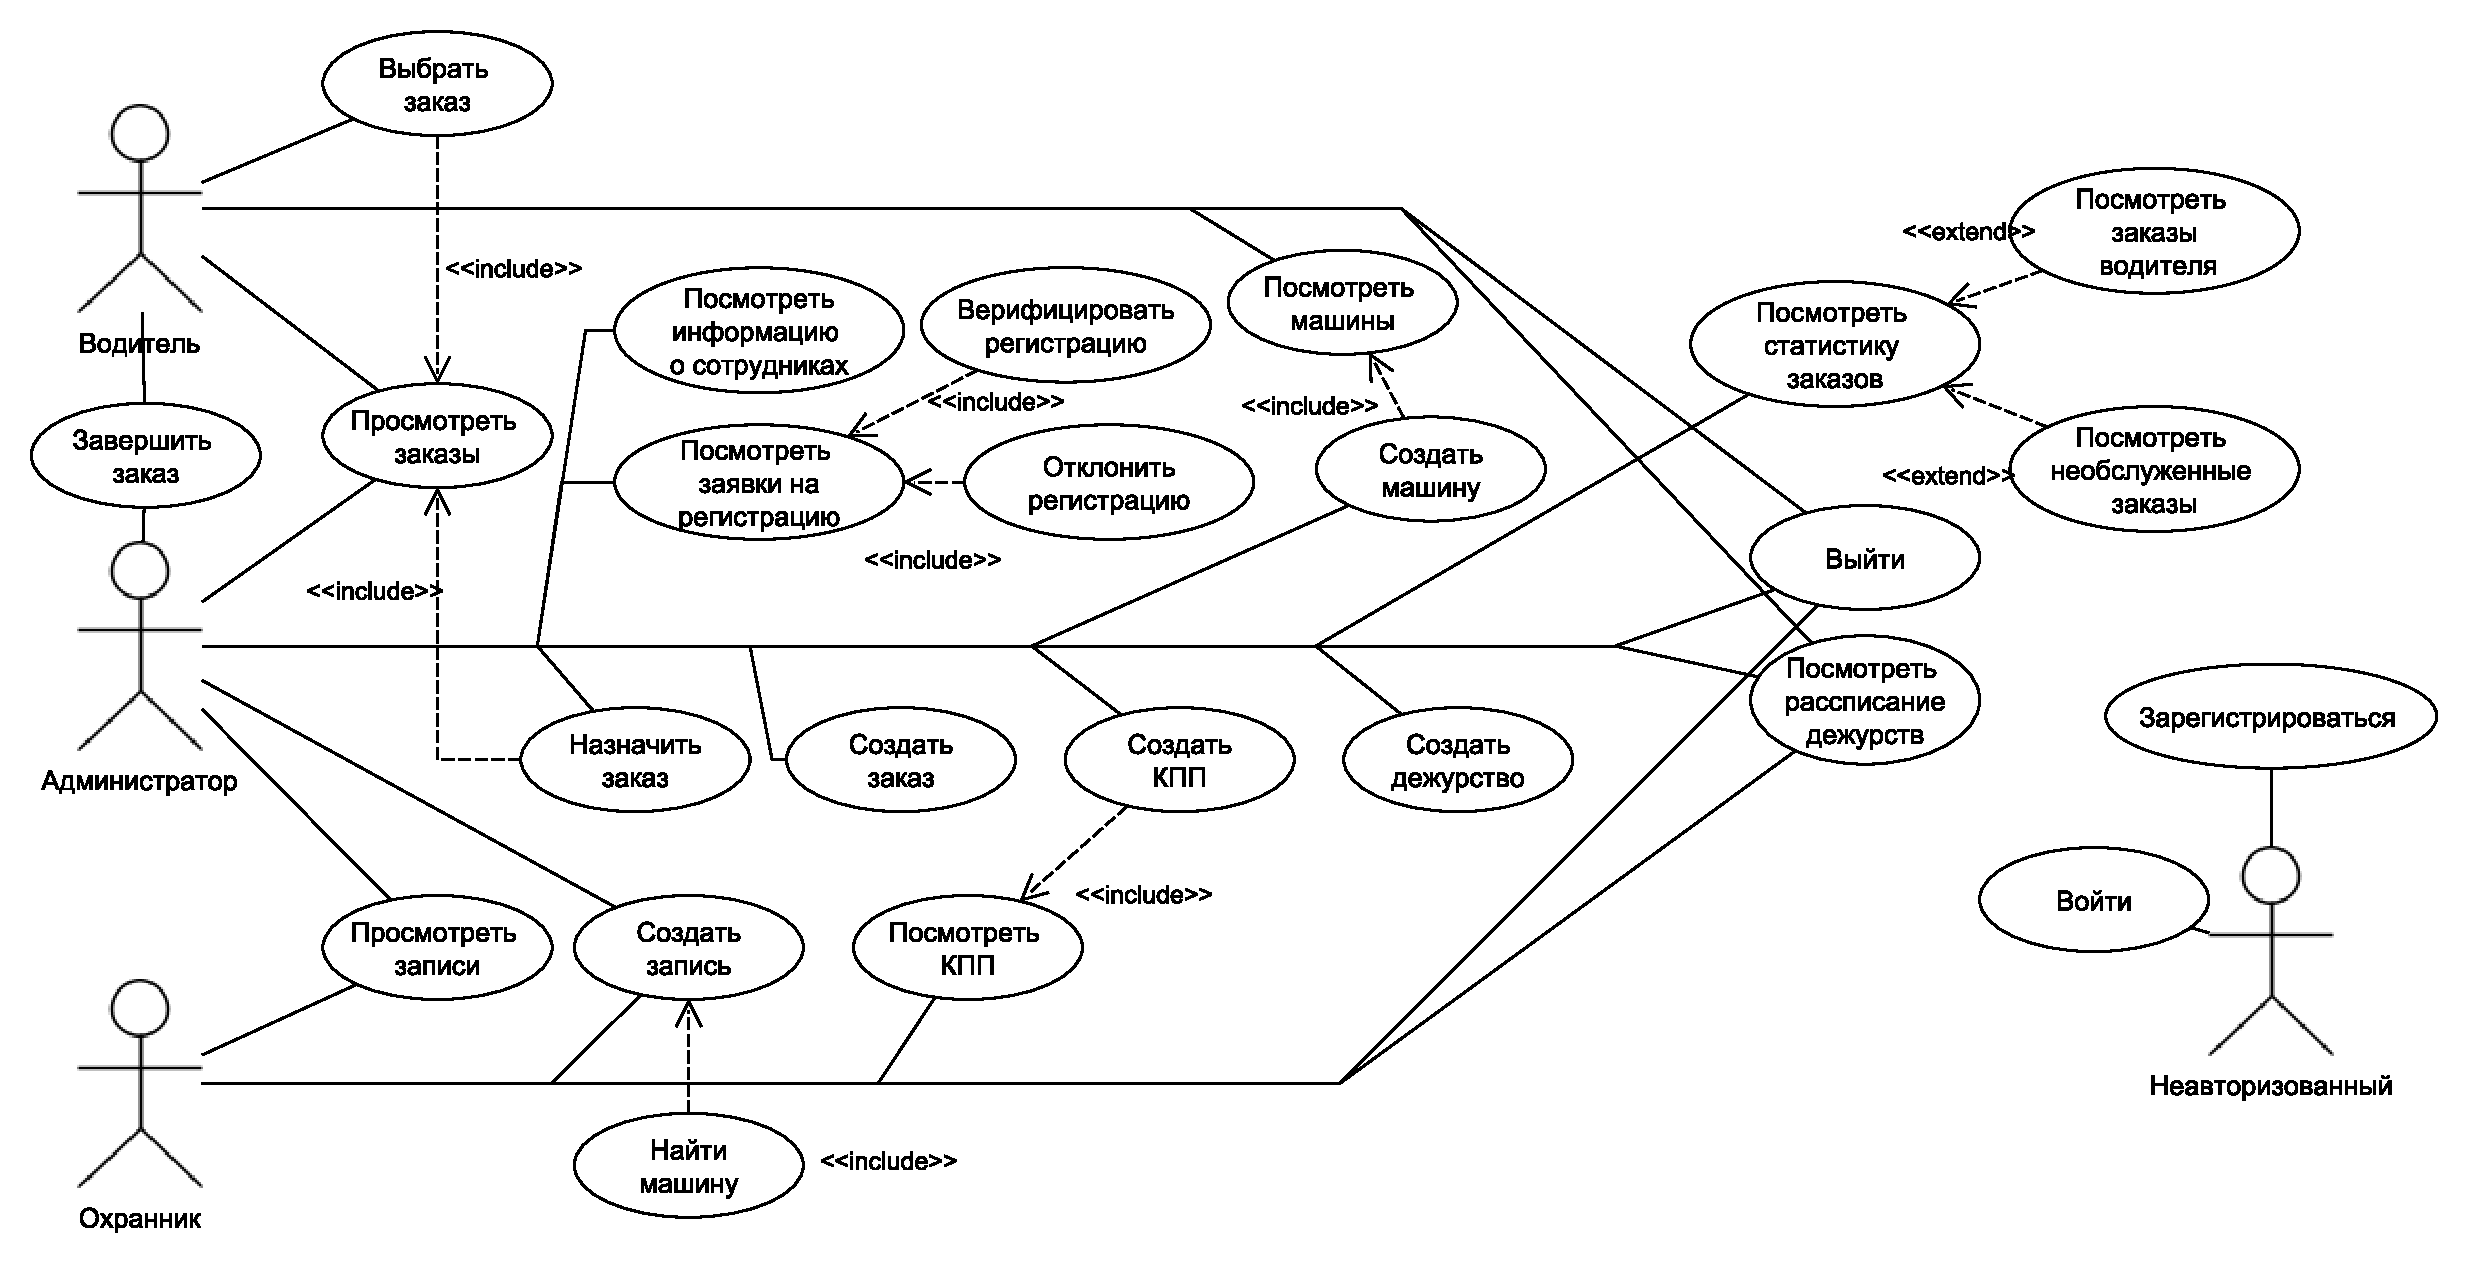
\includegraphics[scale=0.4, angle=-90]{schemes/use-case.pdf}}
		\caption{ER-диаграмма сущностей}
		\label{use_case}
	\end{center}
\end{figure}

\section{Проектирование базы данных}
\subsection{Сущности базы данных}
На рисунке \ref{er_db} представленна ER-диаграмма сущностей базы данных.

\begin{figure}[ph!]
	\begin{center}
		{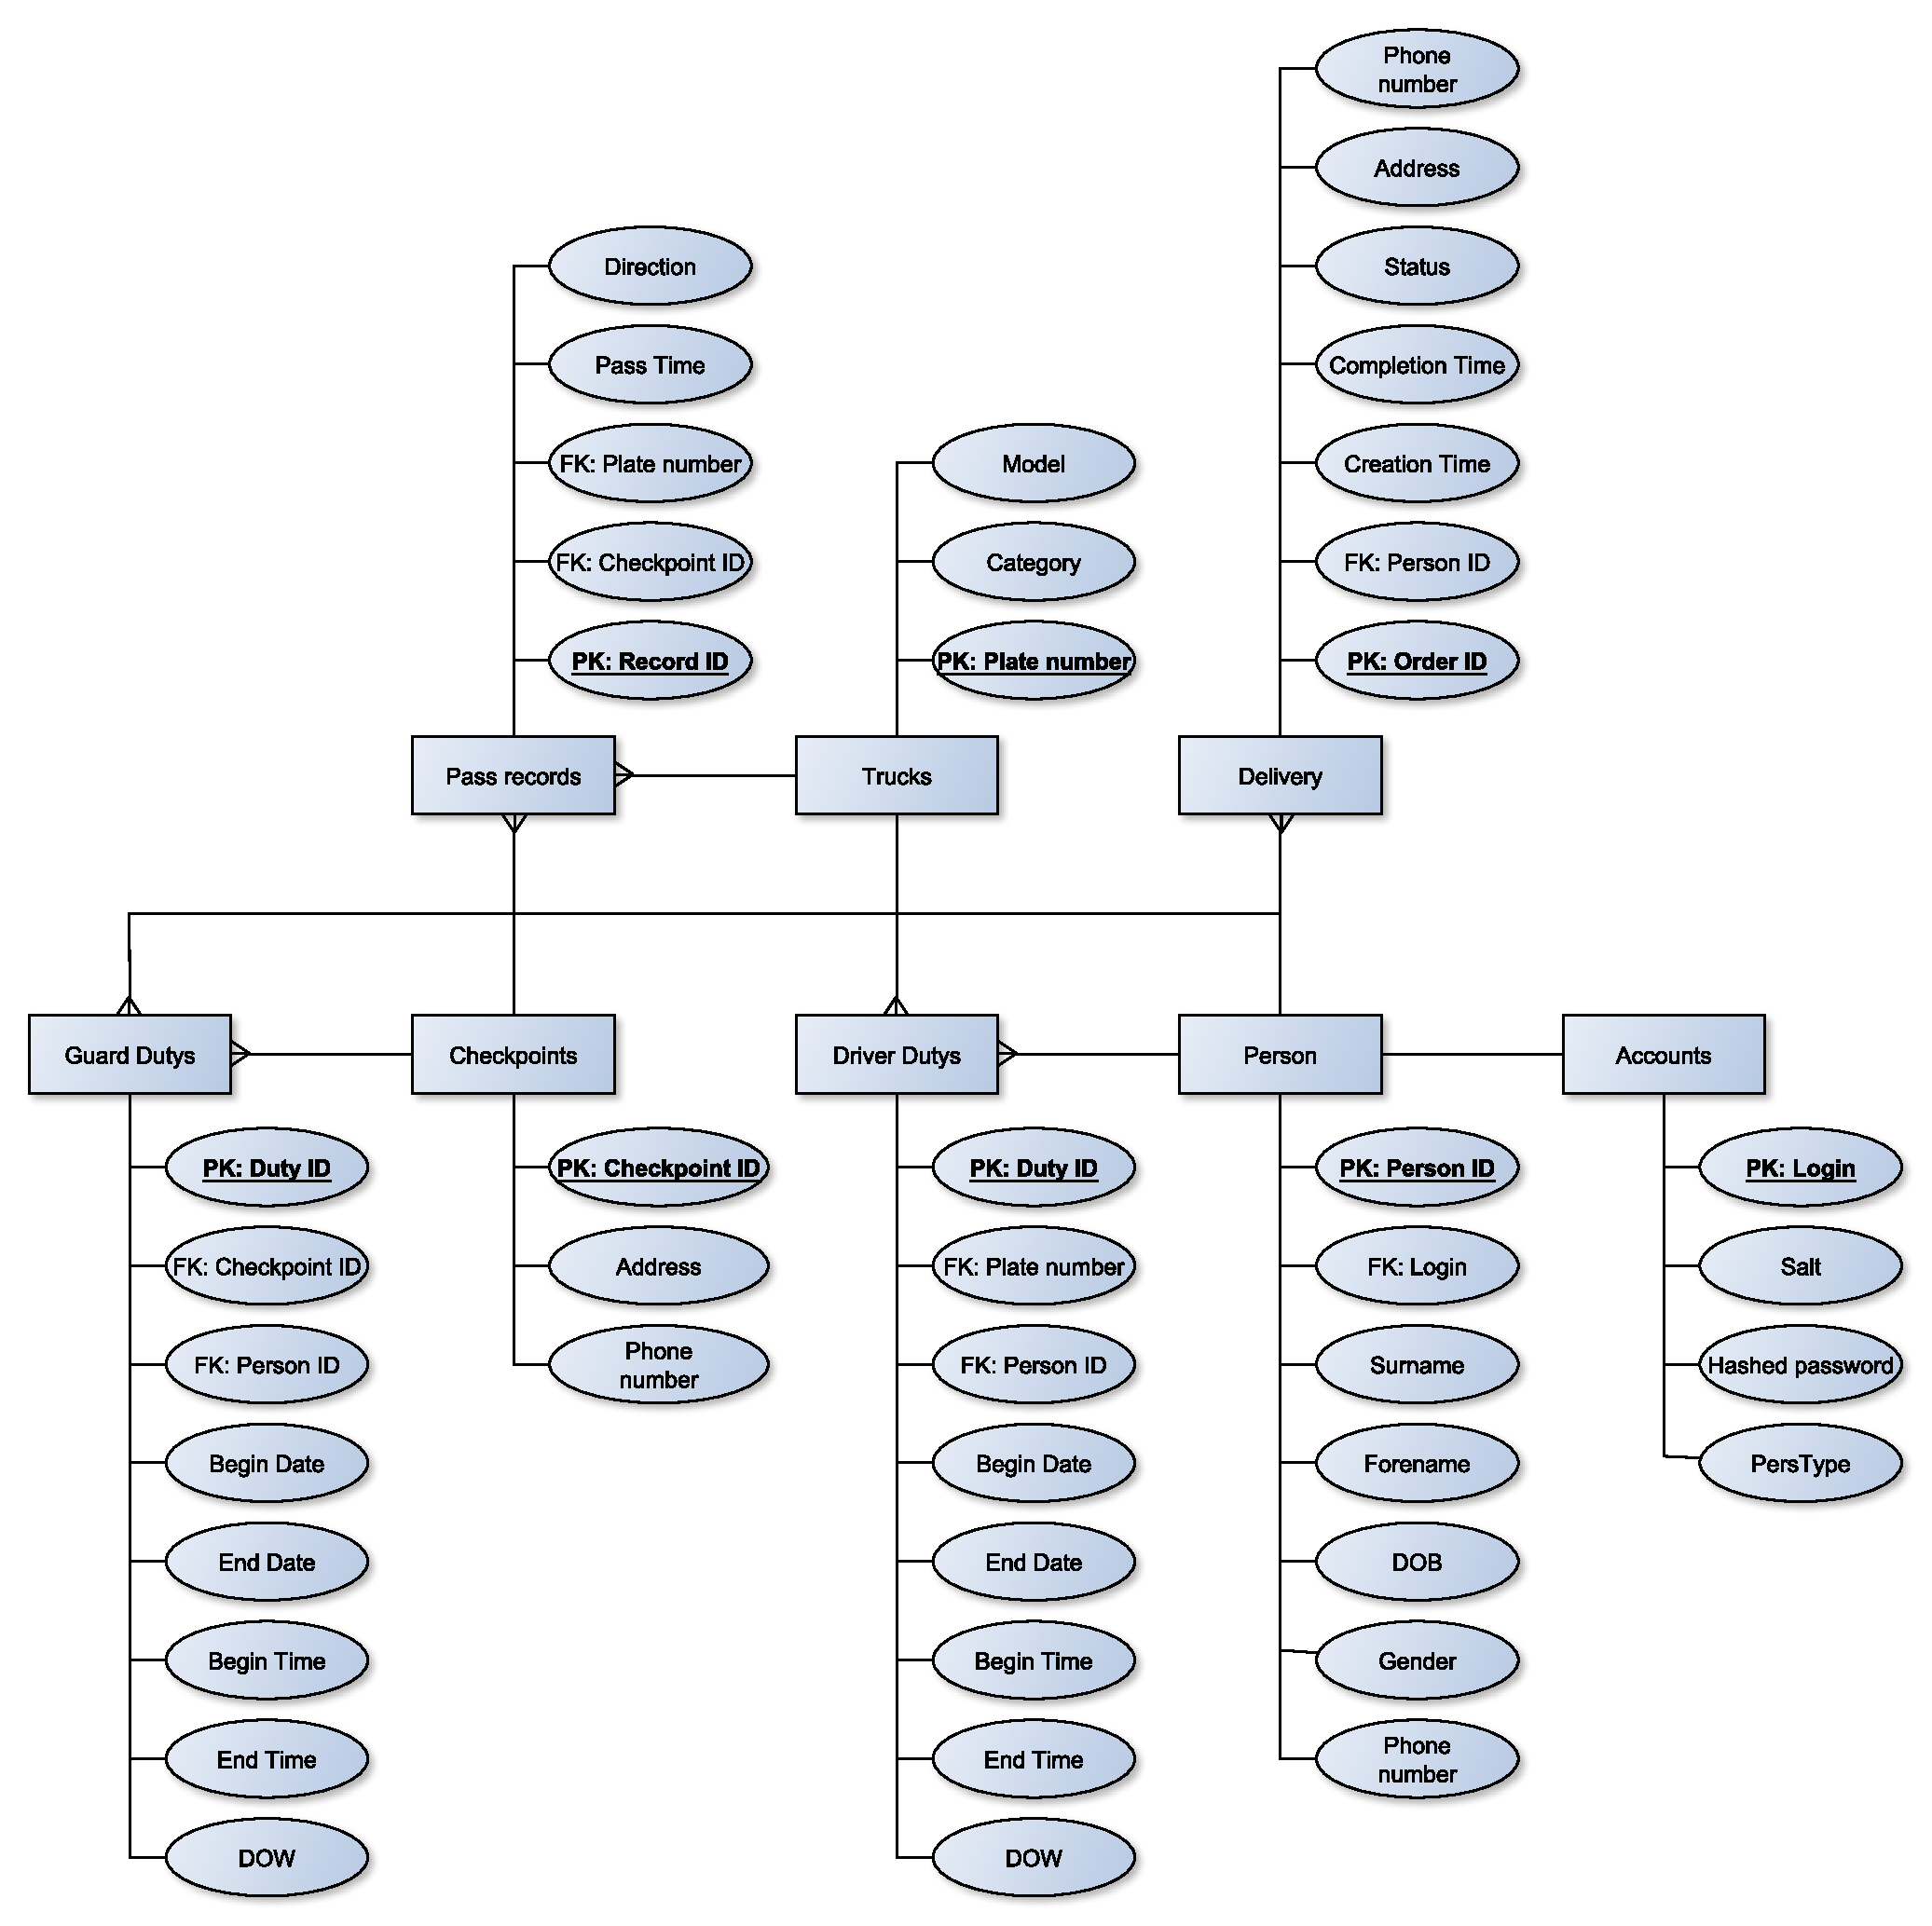
\includegraphics[height=14cm, width = 15cm]{schemes/er_db.pdf}}
%		{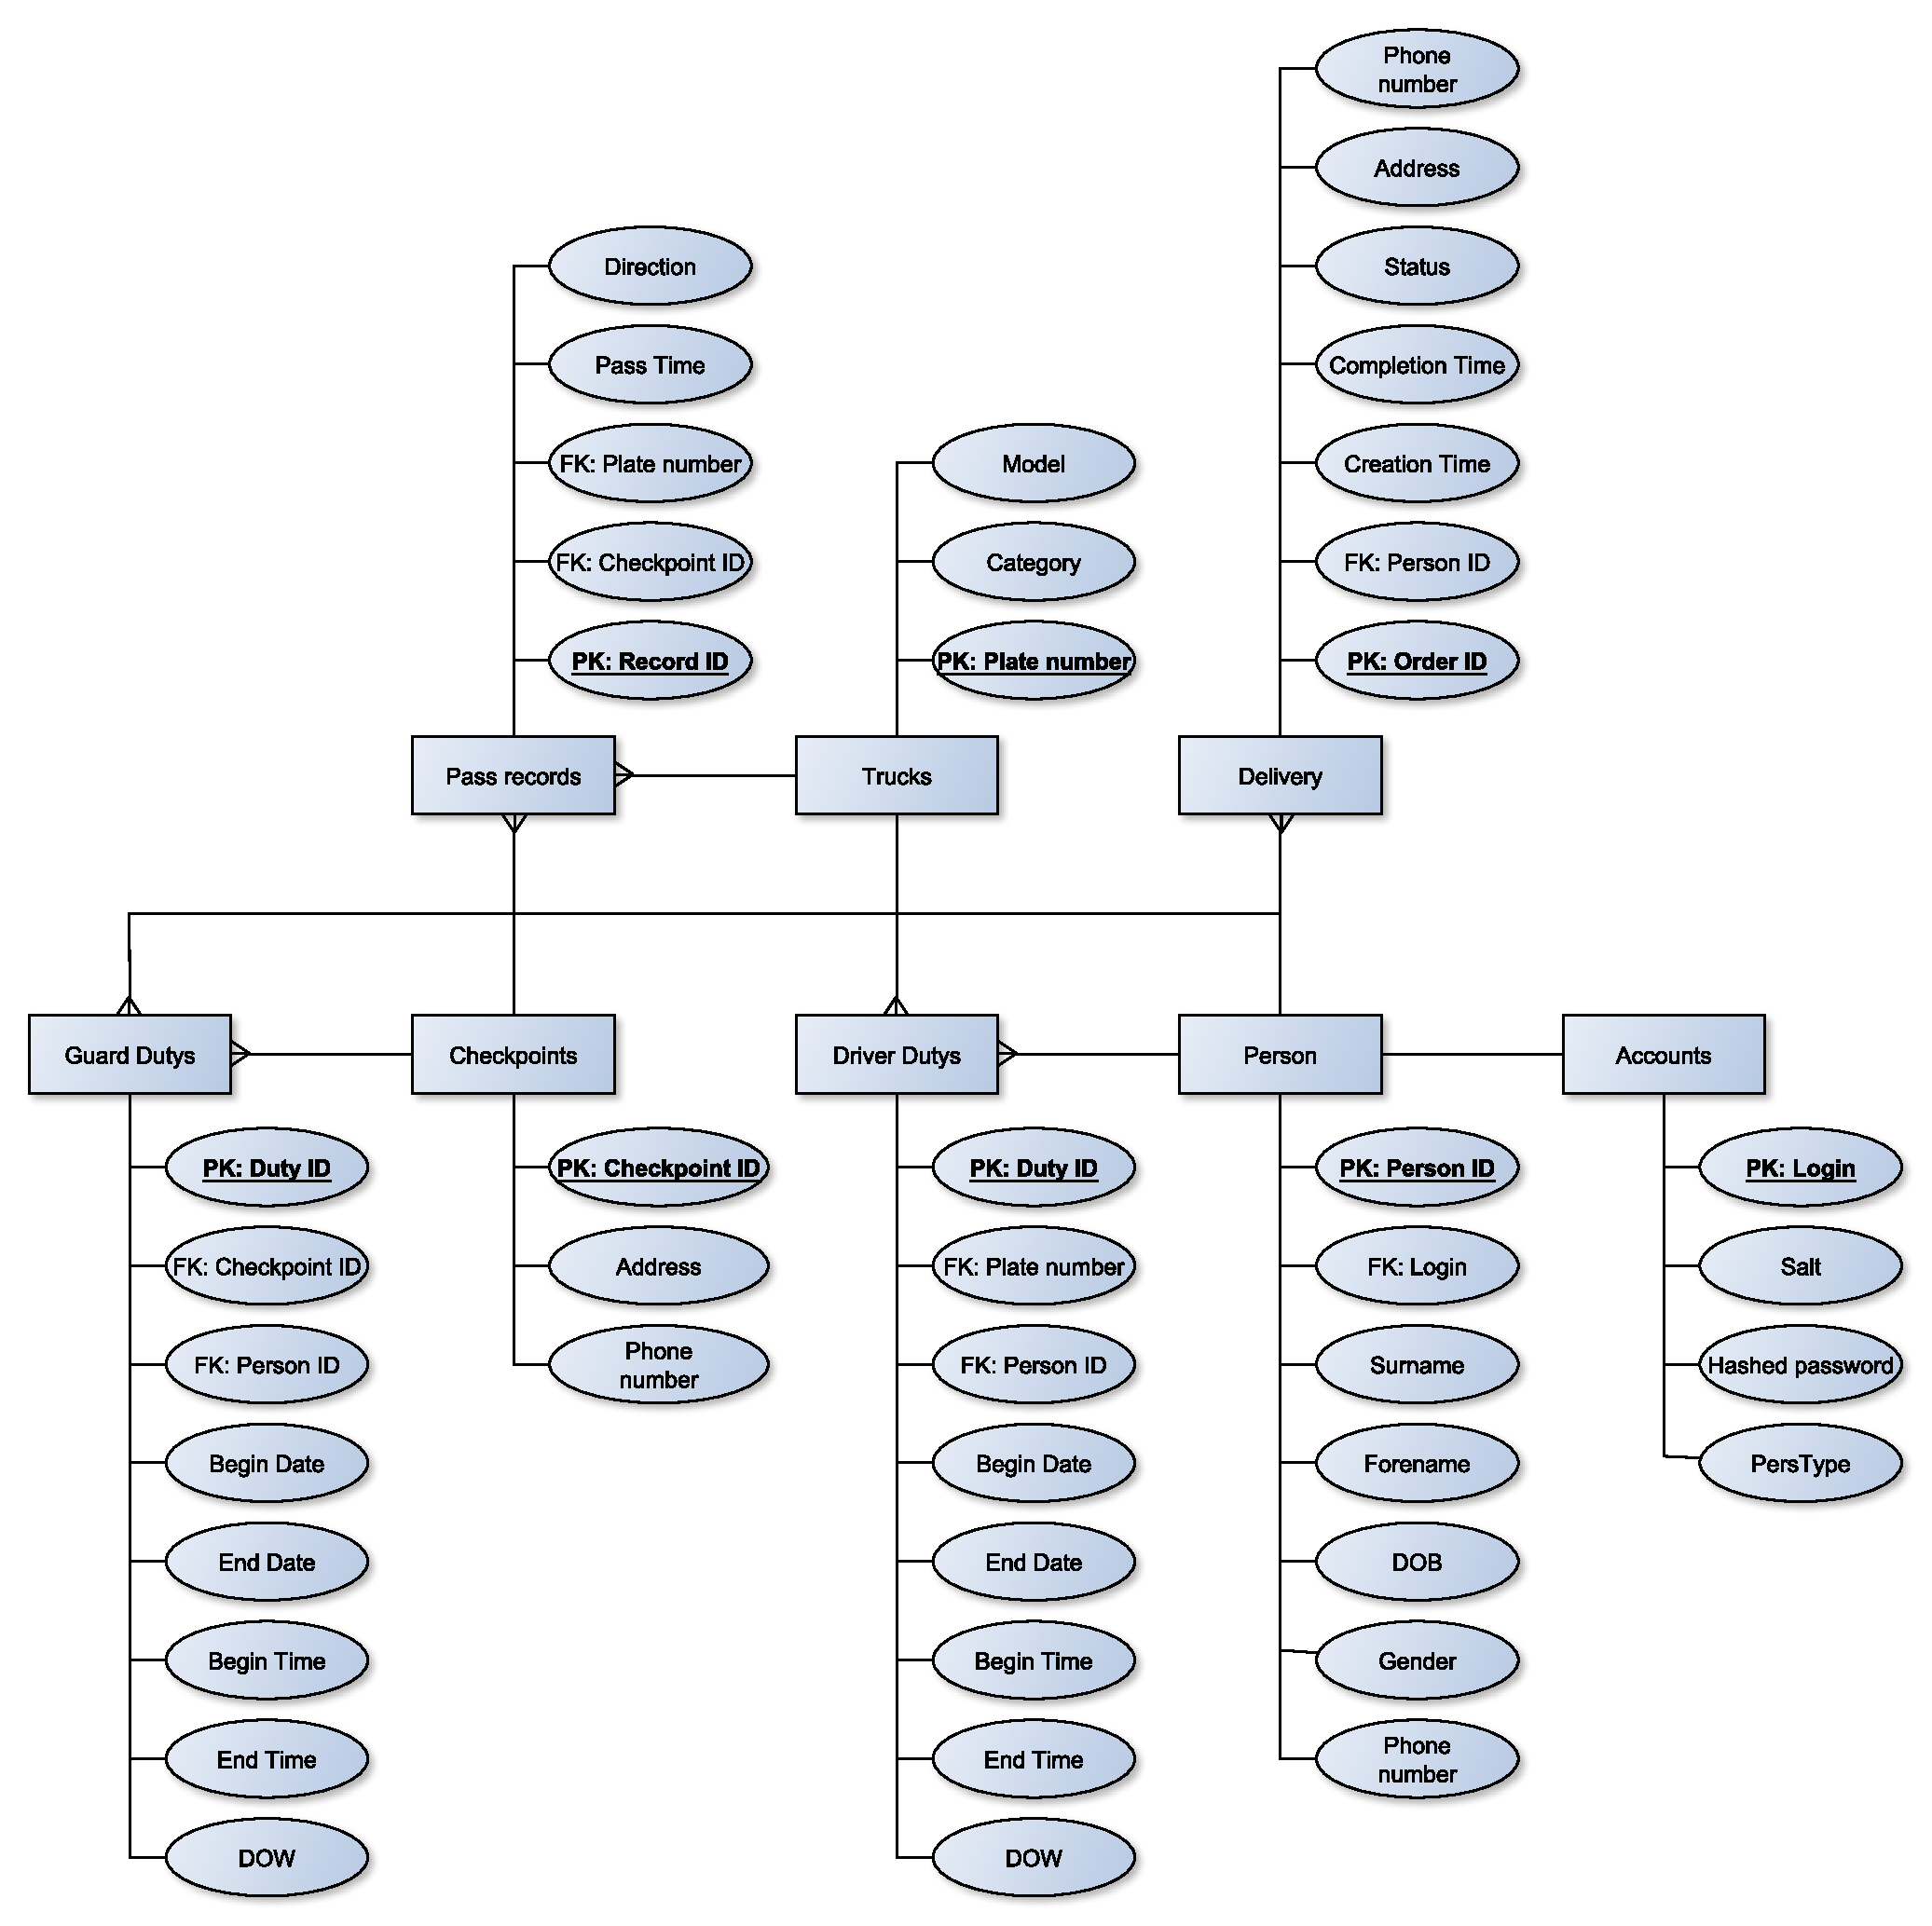
\includegraphics[scale=0.4, angle=0]{schemes/er_db.pdf}}
		\caption{ER-диаграмма сущностей базы данных}
		\label{er_db}
	\end{center}
\end{figure}

\subsection{Проектирование таблиц}
На основании выделенных сущностей база данных должна содержать таблицы, описание которых приведено в таблицах 2.1-2.8

Для обеспечения приватности пароля к аккаунту было принято решение использовать хэширование. В качестве ролей используются значения admin, driver, guard (соотв. администратор, водитель, охранник).
\begin{table}[h] 
	\begin{center}
	\caption{Accounts (таблица аккаунтов)}
	\label{acc_table}
	\begin{tabular}{| p{3.8cm} | p{3cm} | p{7.2cm} |}
		\hline
		\textbf{Атрибут}		&	\textbf{Тип}		& \textbf{Комментарий} \\
		\hline
		Login 		&	Строка		&	Логин аккаунта, PK \\ \hline
		PersType 	&	Строка 		&	Роль аккаунта \\ \hline
		Salt 		&	Строка		&	"Соль" для хэширования пароля \\ \hline
		HashedPassword & Строка		&	Хэшированный пароль \\ \hline
	\end{tabular}
	\end{center}
\end{table}

\begin{table}[h] 
	\begin{center}
		\caption{Person (таблица личной информации)}
		\label{pers_table}
		\begin{tabular}{| p{3.8cm} | p{3cm} | p{7.2cm} |}
			\hline
			\textbf{Атрибут}		&	\textbf{Тип}		& \textbf{Комментарий} \\
			\hline
			Login 		&	Строка		&	Логин аккаунта, PK, FK \\ \hline
			Surname 	&	Строка 		&	Фамилия сотрудника \\ \hline
			Forename 	&	Строка 		&	Имя сотрудника \\ \hline
			DOB 		&	Дата		&	Дата рождения сотрудника \\ \hline
			Gender 		&   Строка		&	Пол сотрудника \\ \hline
			PhoneNumber	&   Строка		&	Номер мобильного телефона сотрудника \\ \hline
		\end{tabular}
	\end{center}
\end{table}

\begin{table}[h!] 
	\begin{center}
		\caption{Trucks (таблица машин)}
		\label{truck_table}
		\begin{tabular}{| p{3.8cm} | p{3cm} | p{7.2cm} |}
			\hline
			\textbf{Атрибут}		&	\textbf{Тип}		& \textbf{Комментарий} \\
			\hline
			PlateNumber	&	Строка	&	Гос. номер машины, PK \\ \hline
			Category	&	Строка	&	Марка машины \\ \hline
			Model		&	Строка	&	Модель машины \\ \hline
		\end{tabular}
	\end{center}
\end{table}

В качестве статуса заказа используются значения not\_assigned, in\_transit, delivered (соотв. заказ не назначен водителю, заказ в процессе доставки и заказ доставлен).
\begin{table}[h!] 
	\begin{center}
		\caption{Delivery (таблица заказов)}
		\label{del_table}
		\begin{tabular}{| p{3.8cm} | p{3cm} | p{7.2cm} |}
			\hline
			\textbf{Атрибут}		&	\textbf{Тип}		& \textbf{Комментарий} \\
			\hline
			OrderID		&	Целое число	&	Уникальный номер заказа, PK \\ \hline
			Login 		&	Строка		&	Логин водителя, доставляющего или доставившего заказ, FK \\ \hline
			Address 	&	Строка 		&	Адрес заказчика \\ \hline
			PhoneNumber	&	Строка 		&	Контакты заказчика \\ \hline
			Status 		& 	Строка		&	Статус заказа \\ \hline
			Description	& 	Строка		&	Содержание заказа \\ \hline
			CreationTime	& Дата, время	&	Дата и время создания заказа \\ \hline
			CompletionTime	& Дата, время	&	Дата и время завершения заказа \\ \hline
		\end{tabular}
	\end{center}
\end{table}

\begin{table}[h!] 
	\begin{center}
		\caption{Checkpoints (таблица КПП)}
		\label{checkp_table}
		\begin{tabular}{| p{3.8cm} | p{3cm} | p{7.2cm} |}
			\hline
			\textbf{Атрибут}		&	\textbf{Тип}		& \textbf{Комментарий} \\
			\hline
			CheckpointID	&	Целое число	&	Номер КПП, PK \\ \hline
			Address			&	Строка		&	Адрес КПП \\ \hline
			PhoneNumber		&	Строка		&	Номер телефона КПП \\ \hline
		\end{tabular}
	\end{center}
\end{table}


Дежурства как охранников, так и водителей имеют цикличный характер по неделе. Поэтому рациональнее хранить не каждое дежурство отдельно, а правило, содержащее диапазон дат и дни недели, в которые сотрудник дежурит. Атрибут дней недели в таблице хранит строку, определяющую дни по номеру (например строка 013 соответсвует дежурству по понедельникам, вторникам и четвергам). Период (или расписание) дежурства выделено в отдельную таблицу.

\begin{table}[h!]
	\begin{center}
		\caption{DutyRules (таблица расписаний дежурств)}
		\label{dutyrule_table}
		\begin{tabular}{| p{3.8cm} | p{3cm} | p{7.2cm} |}
			\hline
			\textbf{Атрибут}		&	\textbf{Тип}		& \textbf{Комментарий} \\
			\hline
			RuleID		&	Целое число	&	Номер периода дежурства, PK \\ \hline
			BeginDate 	&	Дата		&	Дата начала периода дежурства \\ \hline
			EndDate 	&	Дата		&	Дата окончания периода дежурства \\ \hline
			BeginTime 	&	Время		&	Время начала дежурства \\ \hline
			EndTime 	&	Время		&	Время окончания дежурства \\ \hline
			DOW 		&	Строка		&	Дни недели дежурства \\ \hline
		\end{tabular}
	\end{center}
\end{table}

\begin{table}[h!]
	\begin{center}
		\caption{GuardDutys (таблица дежурств охранников)}
		\label{gduty_table}
		\begin{tabular}{| p{3.8cm} | p{3cm} | p{7.2cm} |}
			\hline
			\textbf{Атрибут}		&	\textbf{Тип}		& \textbf{Комментарий} \\
			\hline
			DutyID		&	Целое число	&	Номер дежурства, PK \\ \hline
			Login 		&	Строка		&	Логин дежурящего охранника, FK \\ \hline
			CheckpointID &	Целое число	&	Номер КПП, FK \\ \hline
			RuleID		&	Целое число	&	Номер периода дежурства, FK \\ \hline
		\end{tabular}
	\end{center}
\end{table}

\begin{table}[h!] 
	\begin{center}
		\caption{DriverDutys (таблица дежурств водителей)}
		\label{dduty_table}
		\begin{tabular}{| p{3.8cm} | p{3cm} | p{7.2cm} |}
			\hline
			\textbf{Атрибут}		&	\textbf{Тип}		& \textbf{Комментарий} \\
			\hline
			DutyID		&	Целое число	&	Номер дежурства, PK \\ \hline
			Login 		&	Строка		&	Логин дежурящего водителя, FK \\ \hline
			PlateNumber &	Строка		&	Гос. номер машины, FK \\ \hline
			RuleID		&	Целое число	&	Номер периода дежурства, FK \\ \hline
		\end{tabular}
	\end{center}
\end{table}

В качестве направления проезда используются значения in, out (соотв. въезд и выезд с территории предприятия).
\newpage
\begin{table}[h!] 
	\begin{center}
		\caption{PassRecords (таблица записей проездов)}
		\label{pass_table}
		\begin{tabular}{| p{3.8cm} | p{3cm} | p{7.2cm} |}
			\hline
			\textbf{Атрибут}		&	\textbf{Тип}		& \textbf{Комментарий} \\
			\hline
			RecordID	&	Целое число	&	Номер записи, PK \\ \hline
			PlateNumber	&	Строка		&	Гос. номер машины, FK \\ \hline
			CheckpointID &	Целое число	&	Номер КПП, FK \\ \hline
			PassTime 	&	Дата, время	&	Дата и время проезда \\ \hline
			Direction 	&	Строка		&	Направление проезда \\ \hline
		\end{tabular}
	\end{center}
\end{table}

Также было принято создать таблицу для хранения информации о событиях в базе данных.
\begin{table}[h!] 
	\begin{center}
		\caption{LogActions (таблица активности пользователей)}
		\label{tab:log_action}
		\begin{tabular}{| p{3.8cm} | p{3cm} | p{7.2cm} |}
			\hline
			\textbf{Атрибут}		&	\textbf{Тип}		& \textbf{Комментарий} \\
			\hline
			Actor	&	Строка	&	Роль, осуществившая действие \\ \hline
			ActTime	&	Дата, время		&	Время действия \\ \hline
			Description &	Строка	&	Описание действия \\ \hline
		\end{tabular}
	\end{center}
\end{table}

\subsection{Нормализация схем отношений}
Распространённым подходом в проектировании баз данных является метод нормализации, служащий для устранения избыточности и упрощения контроля целостности. При проектировании данной базы данных была поставленна цель соответствия третьей нормальной форме, что является достаточным для выполнения описанных целей нормализации\cite{norm_db}.

В разработанной модели данных переменная отношения находитя в первой нормальной форме, так как выполняется условие атомарности. В каждом кортеже, соответствующем некоторой описанной таблице, каждый компонент является атомарным, то есть содержит только одно значение для каждого из атрибутов\cite{norm_db2}. Данное утверждение основанно на том, что каждый атрибут имеет простой тип данных.

Также созданная переменная отношения находится во второй нормальной форме, так как в каждой таблице любой не ключевой атрибут полностью зависит от первичного ключа. Для перехода в данную форму из таблиц дежурств охранников и водителей была отдельно выделена таблица расписаний дежурств.

Можно утверждать, что спроектированная переменная отношения находится в третьей нормальной форме. Во всех таблицах не ключевые атрибуты не связаны отношениями между собой, поэтому можно утверждать, что они зависят от первичного ключа нетранзитивно, что и является условием нахождения в третьей нормальной форме.

\subsection{Схемы триггеров}
В соответствии с описанной ранее схемой взаимодействия, существуют некоторые действия, которые могут выполнять сразу несколько ролей. Для сбора дополнительной информации о данных действиях требуется реализовать следующие триггеры. \\



\begin{itemize}
	\item Триггер сохранения информации добавления записи о проезде. Данное действие может осуществлять как охранник, так и администратор, но таблица PassRecords не хранит информации об авторе, поэтому было решено создать данный триггер. Его схема представлена на рисунке \ref{pass_trig}
	
	\begin{figure}[h!]
		\begin{center}
%			{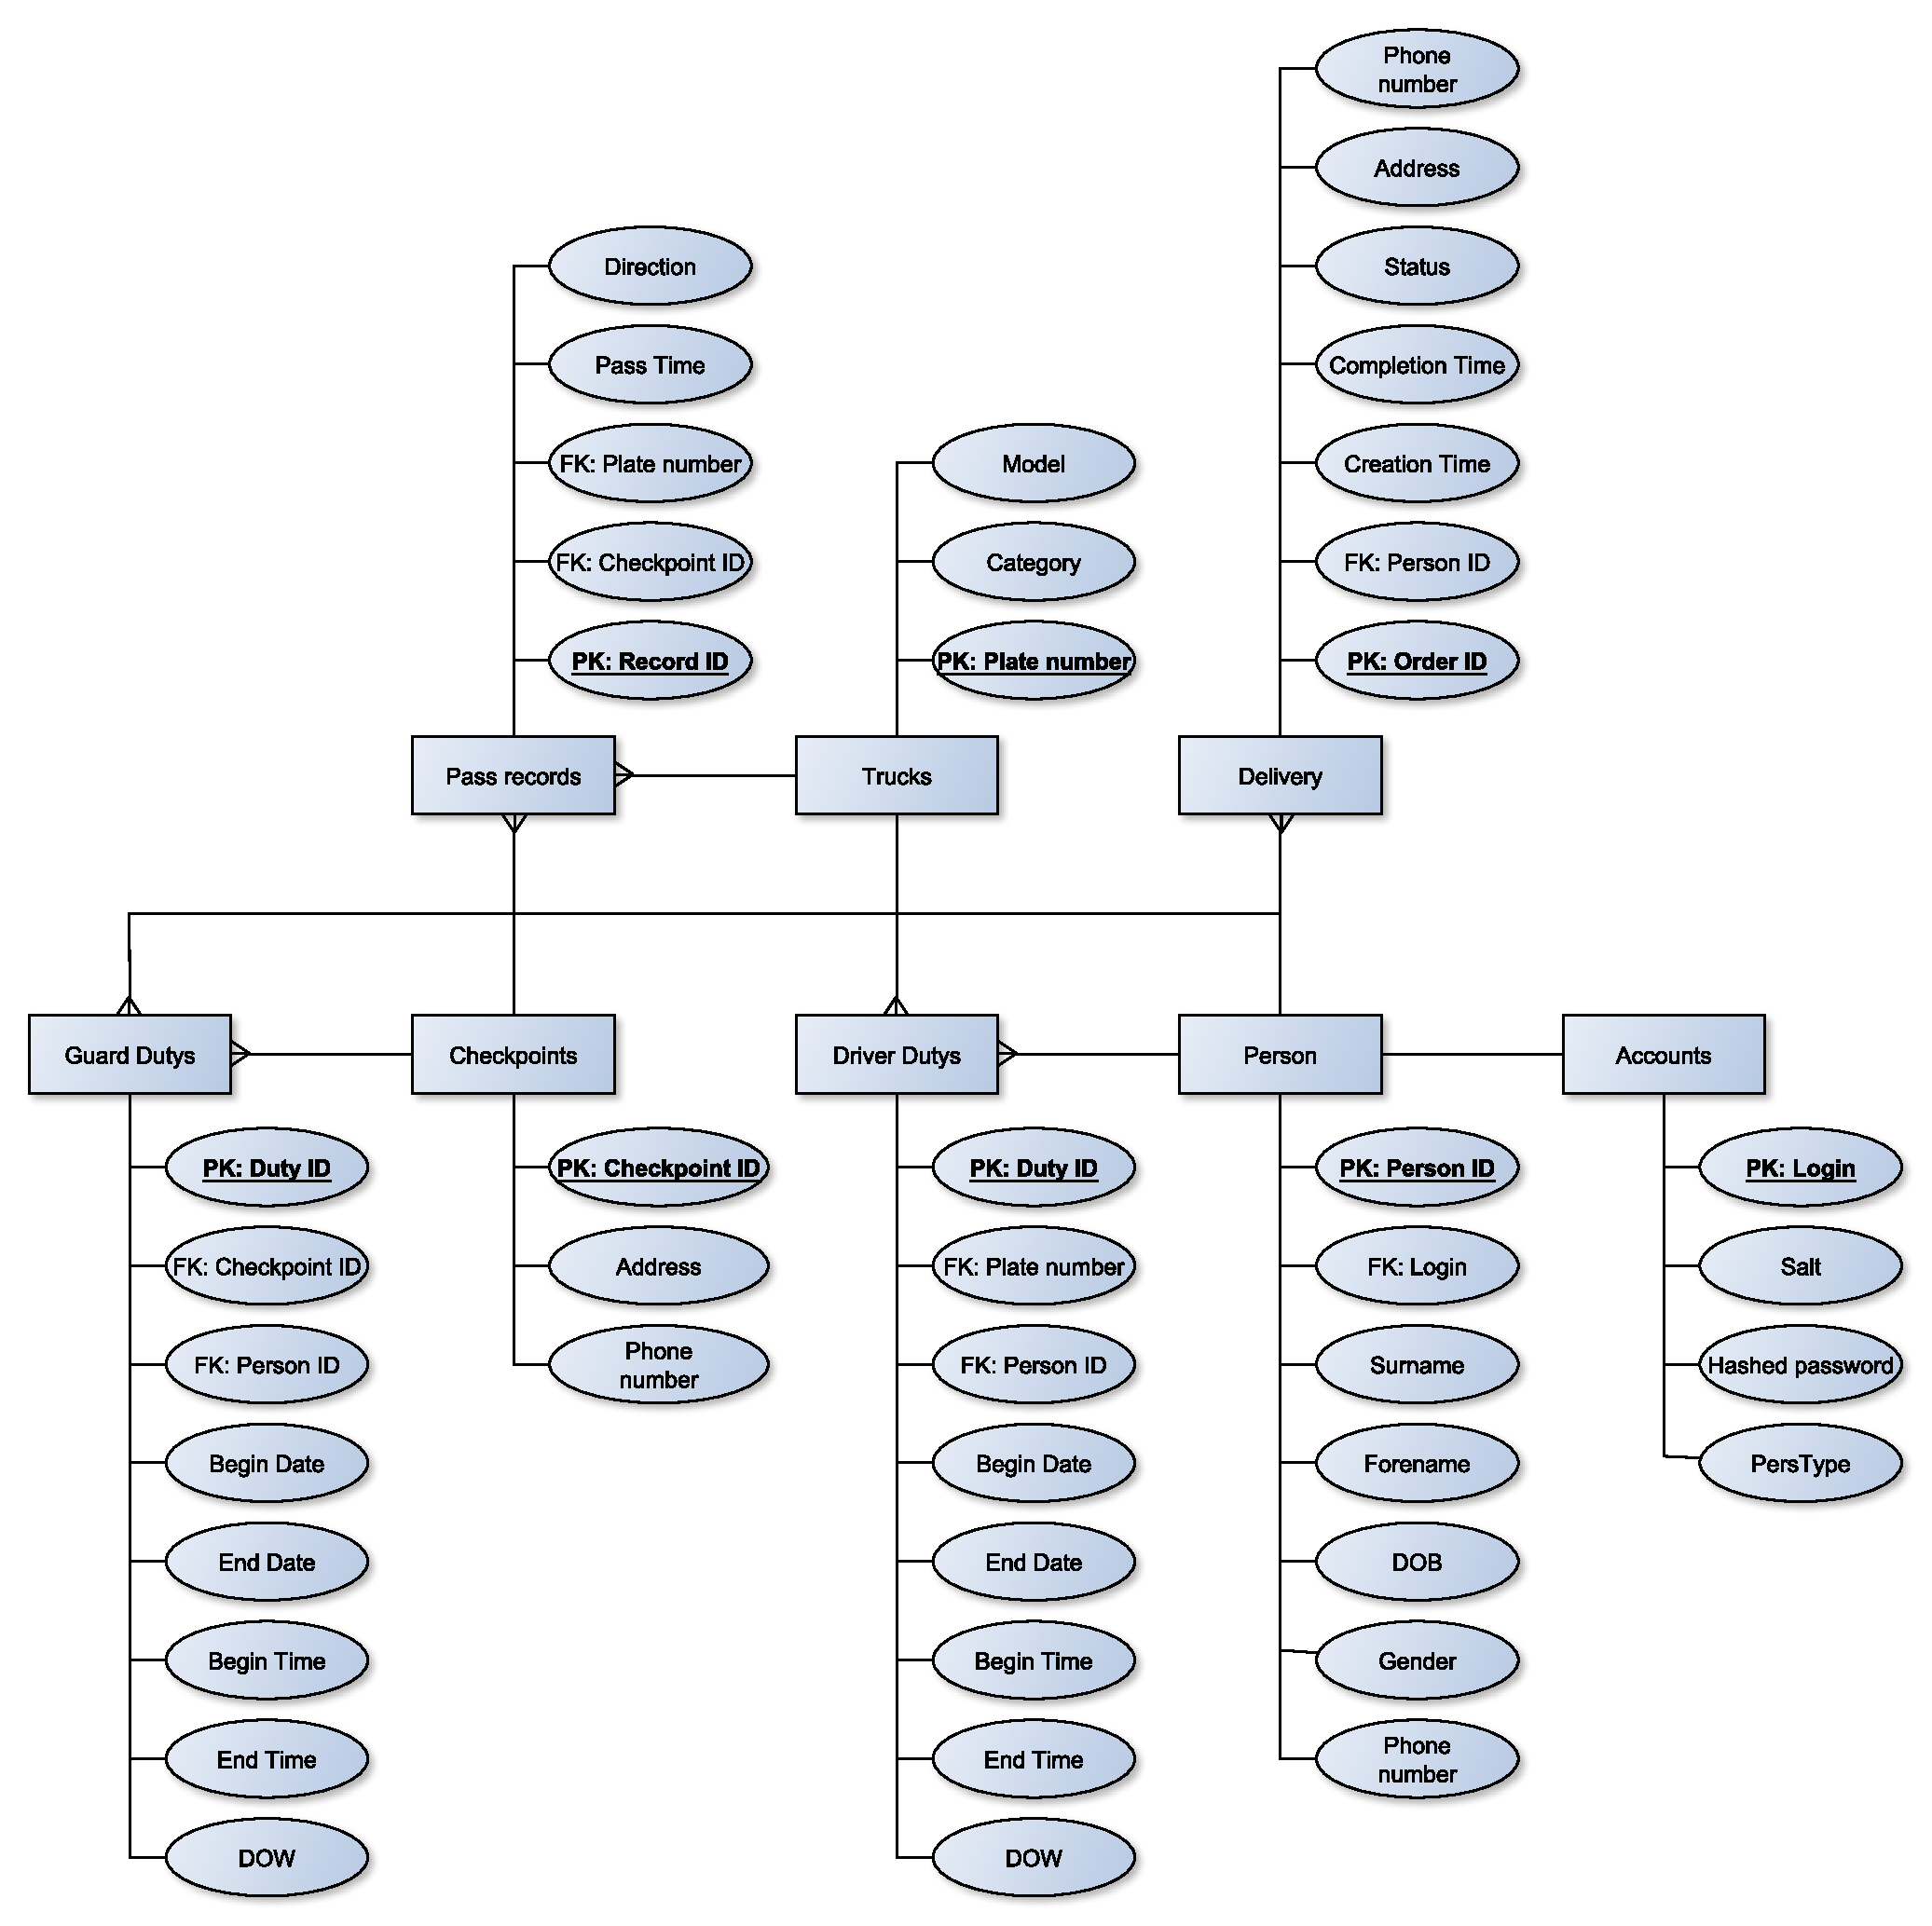
\includegraphics[height=14cm, width = 15cm]{schemes/er_db.pdf}}
			{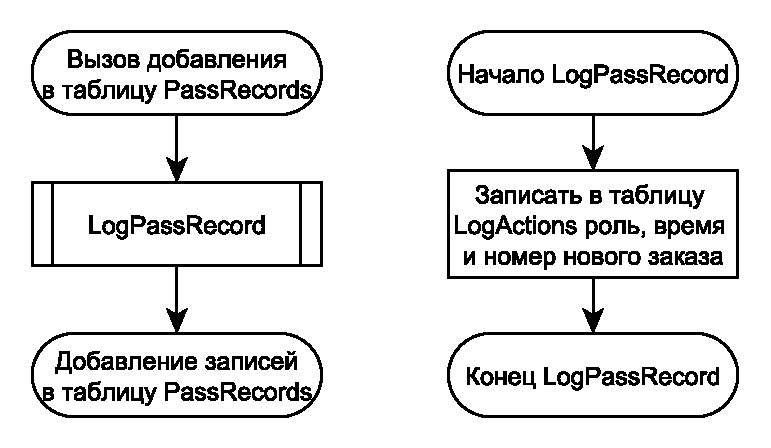
\includegraphics[scale=0.4, angle=0]{sql_schemes/pass_rec}}
			\caption{Схема алгоритма триггера на добавление в таблицу PassRecords}
			\label{pass_trig}
		\end{center}
	\end{figure}

	\item Триггер сохранения информации обновления заказа. В данном случае действие могут совершать водитель и администратор путём изменения статуса заказа и установлением времени его доставки. Его схема представлена на рисунке \ref{del_trig}
	
	\begin{figure}[h!]
		\begin{center}
			%			{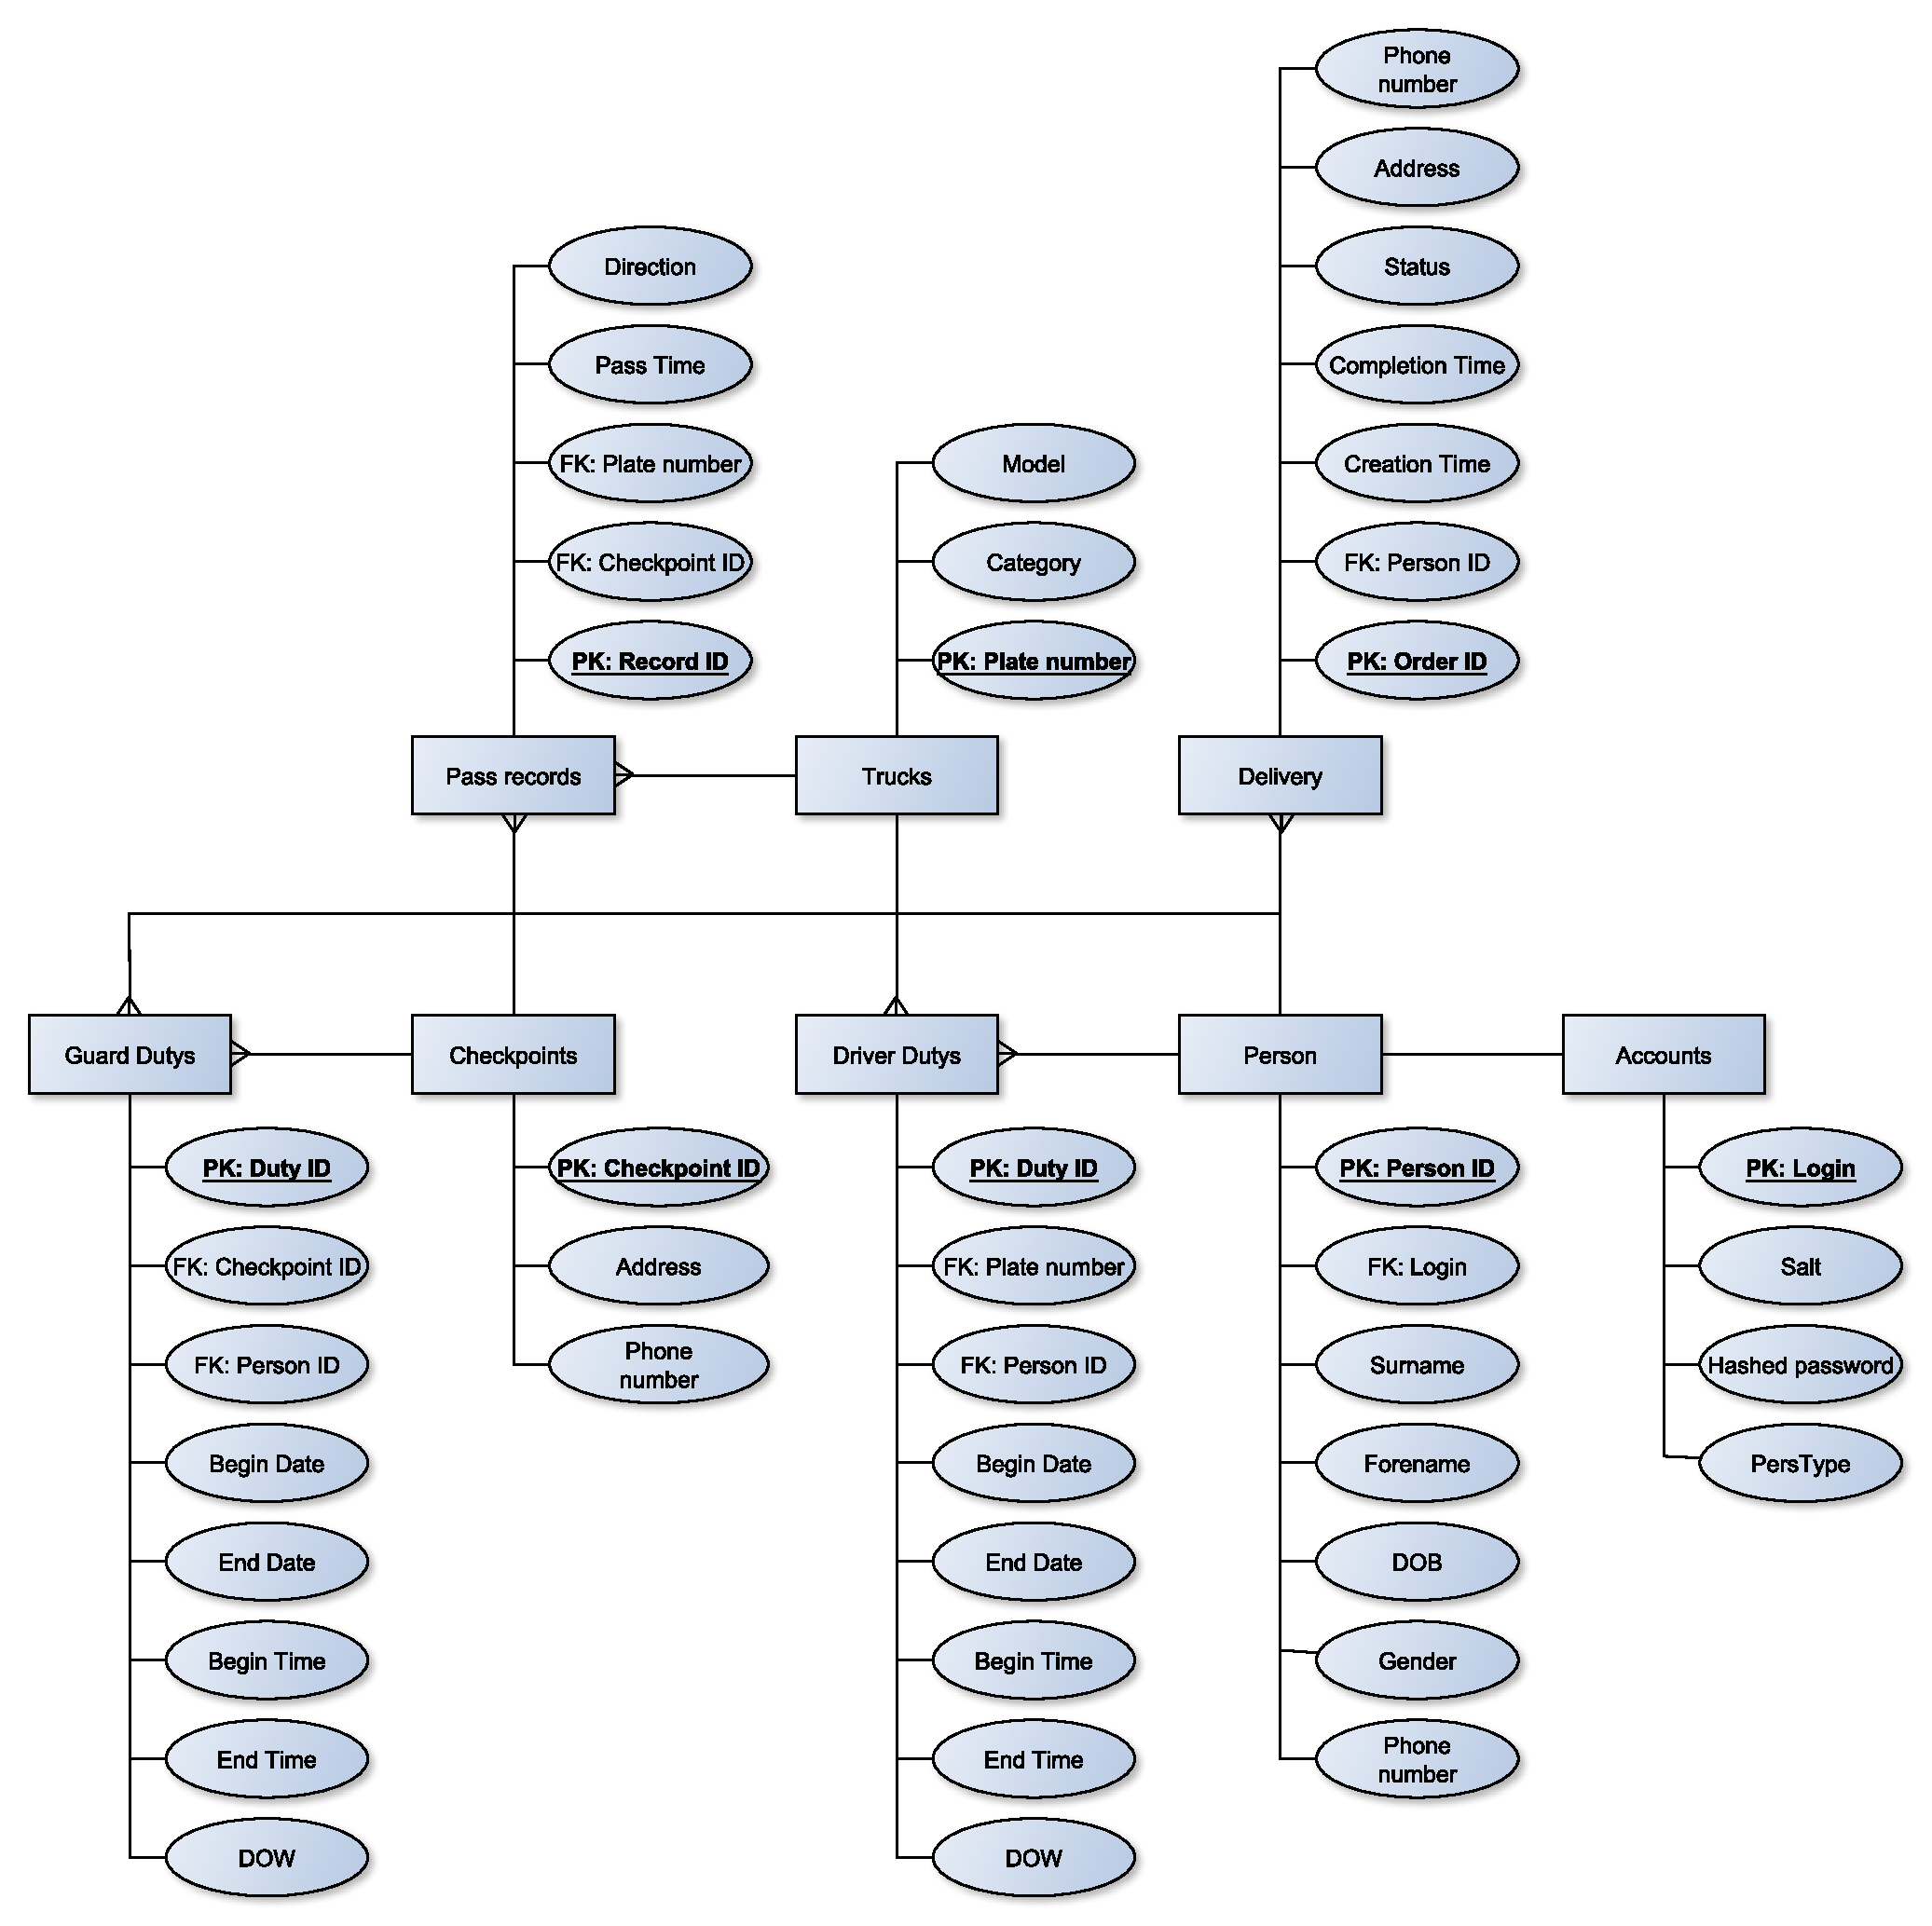
\includegraphics[height=14cm, width = 15cm]{schemes/er_db.pdf}}
			{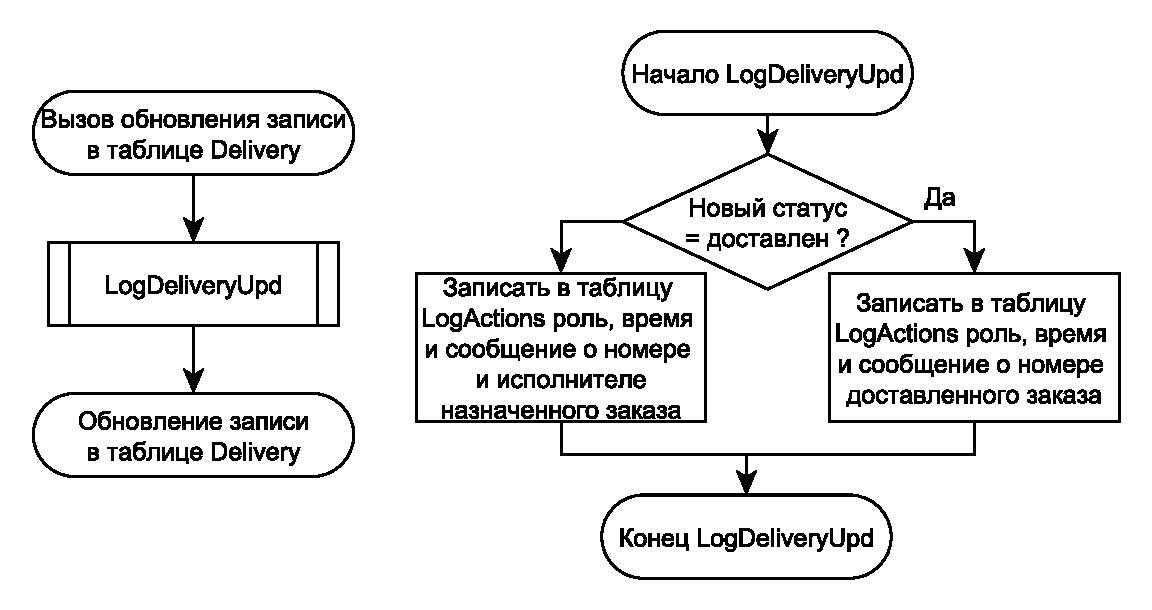
\includegraphics[scale=0.4, angle=0]{sql_schemes/del}}
			\caption{Схема алгоритма триггера на обновление в таблице Delivery}
			\label{del_trig}
		\end{center}
	\end{figure}
\end{itemize}


Также в системе нельзя допускать удаление аккаунтов действующих сотрудников, так как с ними связанна некоторая информация. Например, для доставленных заказов обязательно требуется хранить информацию о его курьере. Поэтому также был создан триггер на удаление записей из таблицы Accounts, запрещающий удалять сотрудников с активным статусом. Схема данного триггера представлена на рисунке \ref{acc_trig}
\begin{figure}[h!]
	\begin{center}
		%			{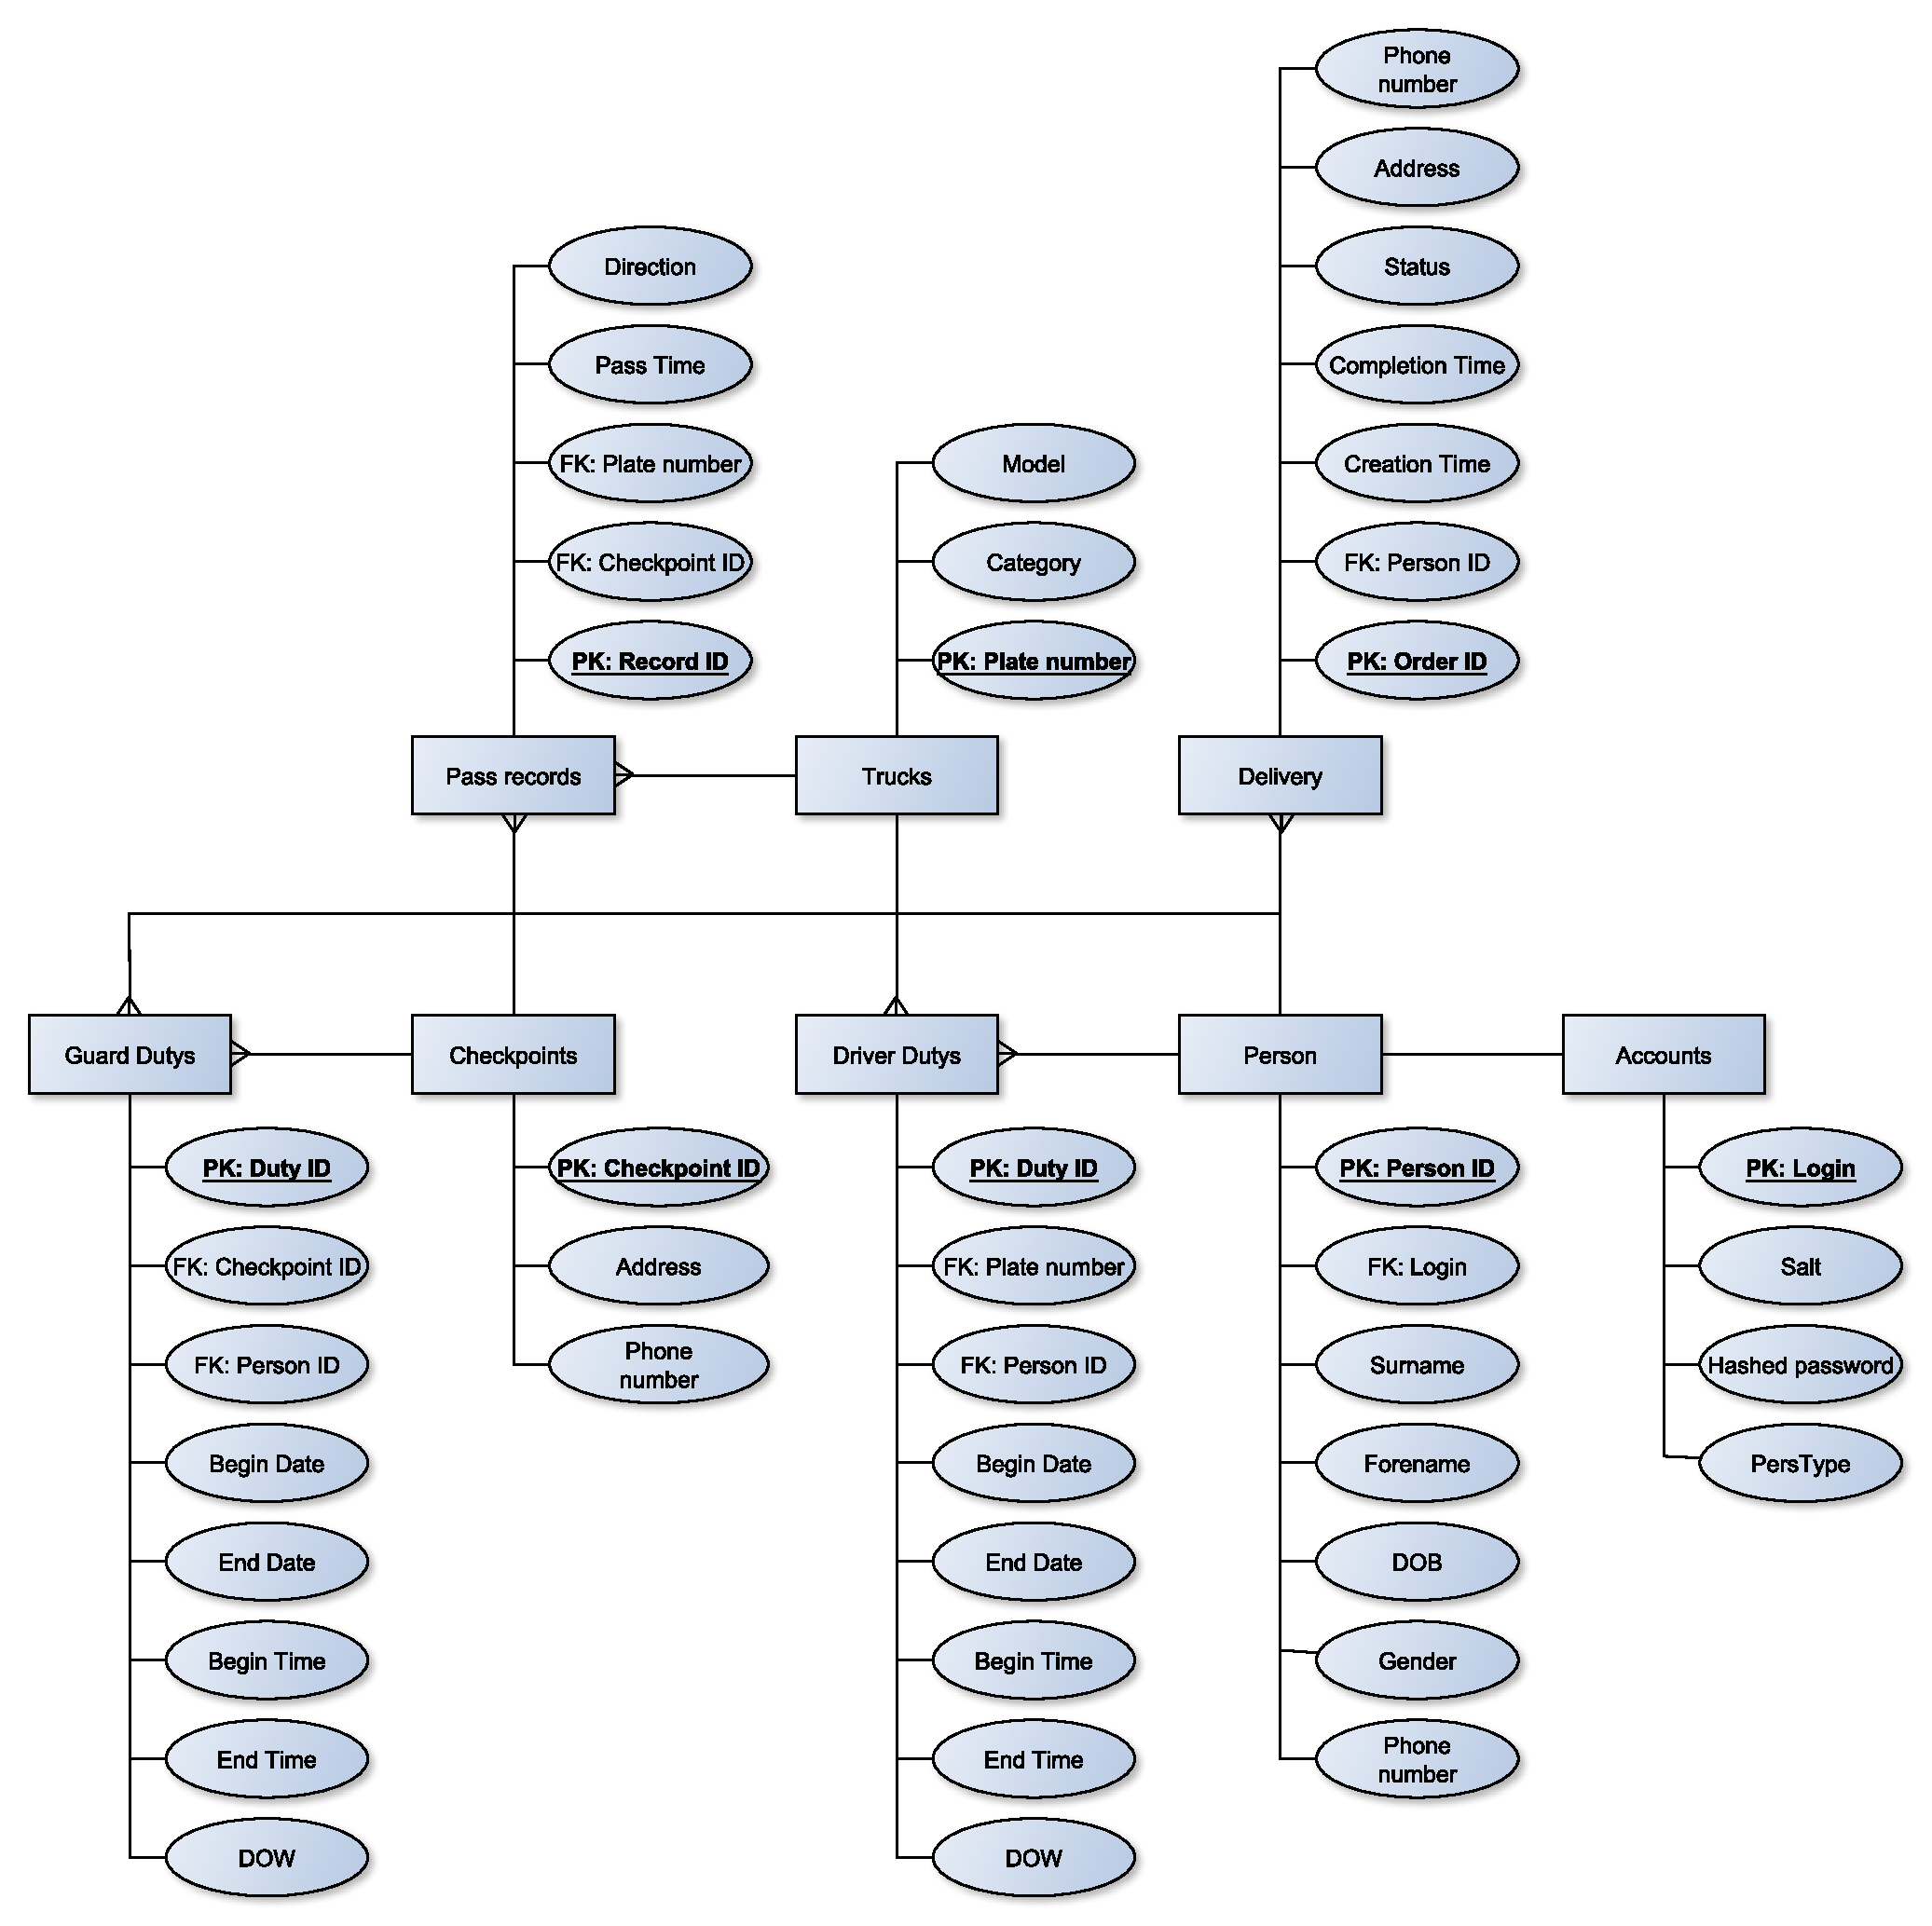
\includegraphics[height=14cm, width = 15cm]{schemes/er_db.pdf}}
		{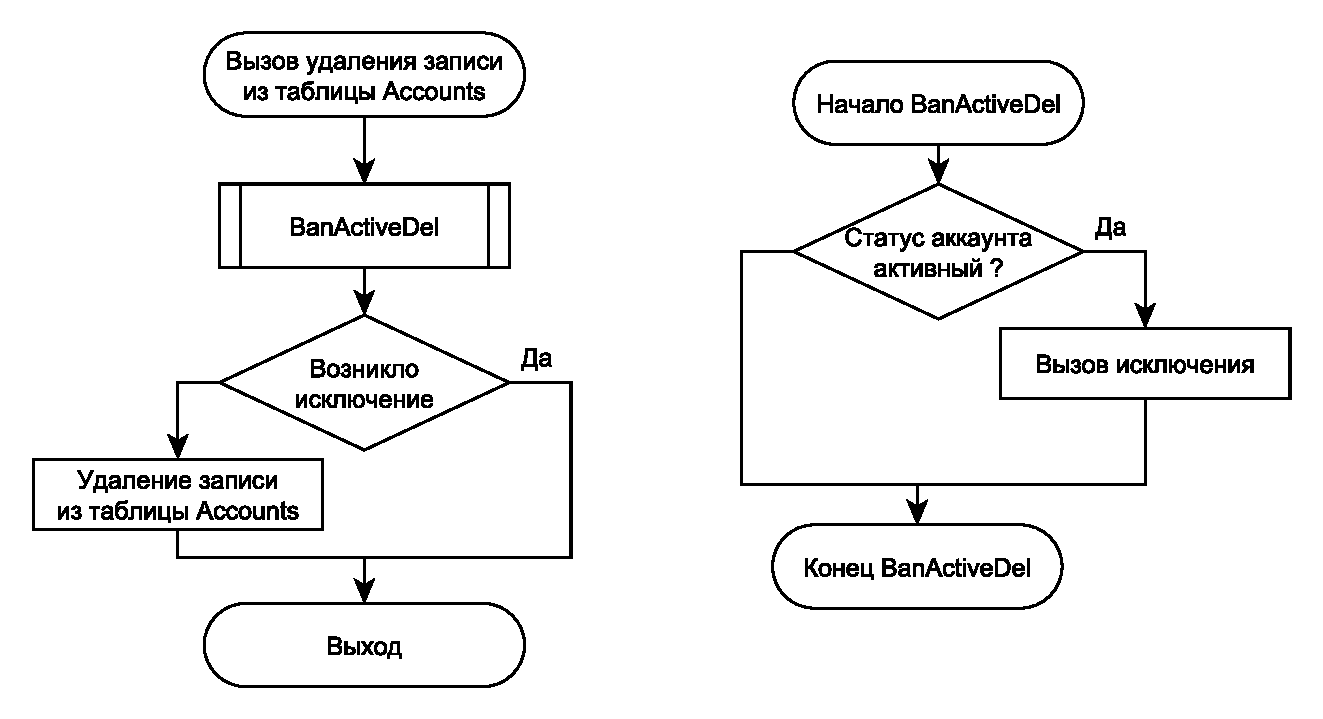
\includegraphics[scale=0.4, angle=0]{sql_schemes/acc}}
		\caption{Схема алгоритма триггера на удаление из таблицы Accounts}
		\label{acc_trig}
	\end{center}
\end{figure}


\section{Архитектура приложения}
Наиболее известным подходом к проектированию архитектуры web-приложения является шаблон MVC. Данный паттерн предполагает разделение приложения на три описанные части.
\begin{itemize}
	\item Model (модель) - компонент бизнес-логики, отвечает за взаимодействие с базой данной и основную обработку информации.
	\item View (представление) - компонент, отвечающий за отображения данных, полученных в результате работы модели.
	\item Controller (контроллер) - компонент, отвечающий за получение запроса от пользователя, передачу их модели для дальнейшего обновления представления.
\end{itemize}

В данной курсовой работе будет использован описанный подход, так как он чётко разграничивает зоны каждого компонента, что позволяет сделать их независимыми.


\section*{Вывод}
Результатом конструкторской части стала разработка сценариев использования приложения, его архитектуры и проектирование таблиц и триггеров базы данных.




	\newpage

	\chapter{Технологическая  часть}
	

\section{Выбор средств программной реализации}

\subsection{Язык программирования}
В качестве языка программирования был выбран Python 3\cite{python_doc}, по следующим причинам.
\begin{itemize}
	\item Поддержка ООП, требуемого для архитектурного шаблона MVC.
	\item Наличие опыта работы с данным языком.
	\item Данный язык является популярным в разработке web-приложений, поэтому он обладает большим количеством web-фреймворков и библиотек для доступа к СУБД.
\end{itemize}

\subsection{СУБД и ORM}
Наиболее популярными реляционными СУБД являются Oracle, Microsoft SQL и PostgreSQL\cite{dbm_source}. Их сравнение\cite{dbm_source2} можно свести в таблицу \hyperref[dms_table]{3.1}

\begin{center}
\begin{longtable}[h]{| p{2.4cm} | p{6.6cm} | p{6.6cm} |}
	\caption{Сравнение реляционных СУБД} \label{dms_table2} \\
 	\hline 
	\multicolumn{1}{|c|}{\textbf{СУБД}} &
	\multicolumn{1}{c|}{\textbf{Преимущества}} &
	\multicolumn{1}{c|}{\textbf{Недостатки}} \\
	\hline
	\endfirsthead
	
	\multicolumn{3}{c}%
	{{\tablename\ \thetable{} -- продолжение}} \\
 	\hline 
	\multicolumn{1}{|c|}{\textbf{СУБД}} &
	\multicolumn{1}{c|}{\textbf{Преимущества}} &
	\multicolumn{1}{c|}{\textbf{Недостатки}} \\
	\hline
	\endhead
	
	\hline \multicolumn{3}{|r|}{{Продолжение на следующей странице}} \\ \hline
	\endfoot
	
	\hline \hline
	\endlastfoot
	
	\hline
	Oracle		&	+ надёжность системы	& -	конечная стоимость СУБД	\\ 
	&	+ поддержка современности функционала	& - высокие системные требования \\ 
	\hline
	
	Microsoft SQL	&	+ прост в использовании	& -	высокая стоимость для юр. лиц	\\ 
	&	+ производительность и надёжность	& - высокая ресурсоёмкость \\ 
	&	+ возможность отслеживания и регулирования уровня производительности & \\
	&	+ эко-система Microsoft & \\
	\hline
	
	PostgreSQL	&	+ лёгкая масштабируемость	& -	скорость выполнения пакетных операций	\\ 
	&	+ пользовательский интерфейс	& - недостаток документации \\ 
	&	+ поддержка текстовых форматов (в т.ч. json) & \\
\end{longtable}
\end{center}

Наиболее подходящим для небольших организаций, которые являются целевыми для разрабатываемой программы, является PostgreSQL\cite{dbm_source2}. Учитывая наличие опыта работы с данным средством, оно был выбран в качестве СУБД для данного курсового проекта.

В качестве ORM (технология объектно-реляционного преобразования) был выбран peewee\cite{peewee_doc}, так как она является простой в освоении и использовании, а также позволяет легко подменить СУБД в случае, если это станет необходимо. 

\subsection{Web-фреймворк}
В качестве web-фреймворка был выбран Django, по следующим причинам.
\begin{itemize}
	\item Django использует шаблон проектирования MVC.
	\item Лёгкая масштабируемость.
	\item Django содержит готовые решения для наиболее востребованных задач (например, аутентификация пользователя).
	\item Поддержка шаблонизации html страниц при помощи Jinja2 позволяет легко осуществлять Web MPA разработку.
\end{itemize}


\section{UML-диаграммы компонентов приложения}
\newpage
\subsection{Компонент доступа к данным}
В данной работе компонент доступа к данным реализован с использованием паттерна проектирования Repository. UML диаграмма компонента изображена представленна на рисунке \hyperref[rep_pic]{3.1}  

\begin{figure}[h!] \label{rep_pic}
	\begin{center}
%		{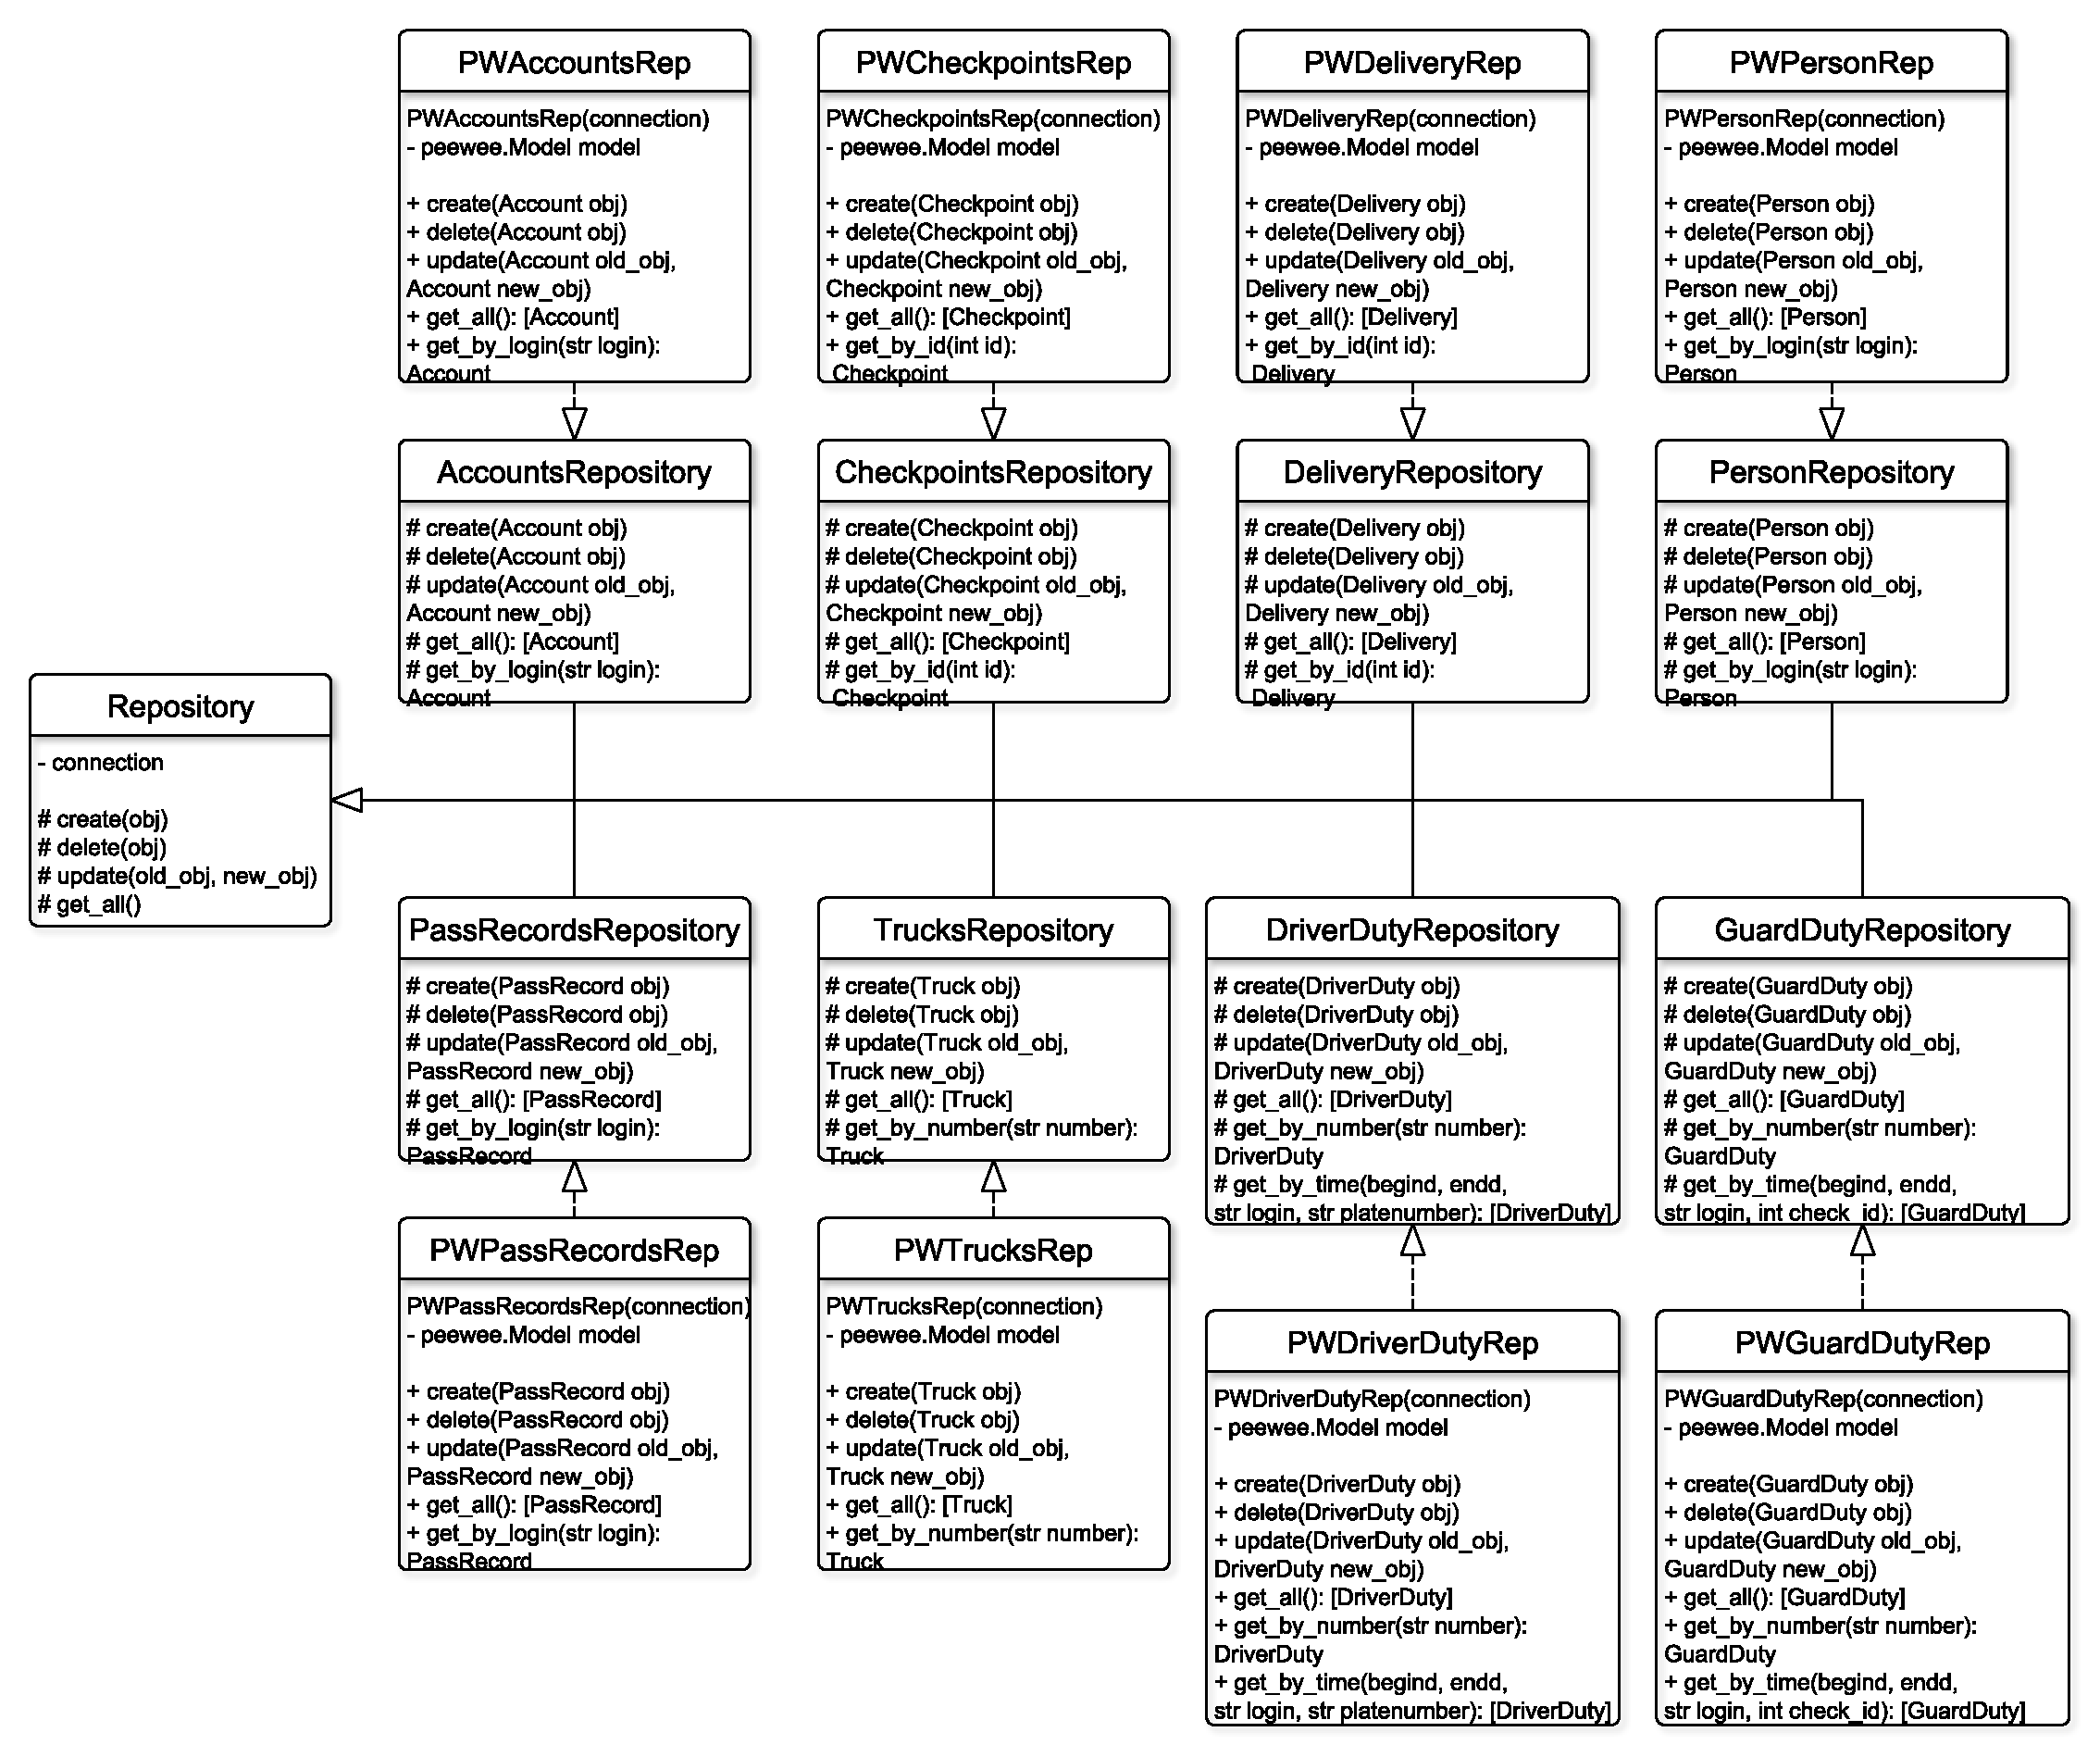
\includegraphics[height=14cm, width = 14cm]{uml/repsoitory.pdf}}
		{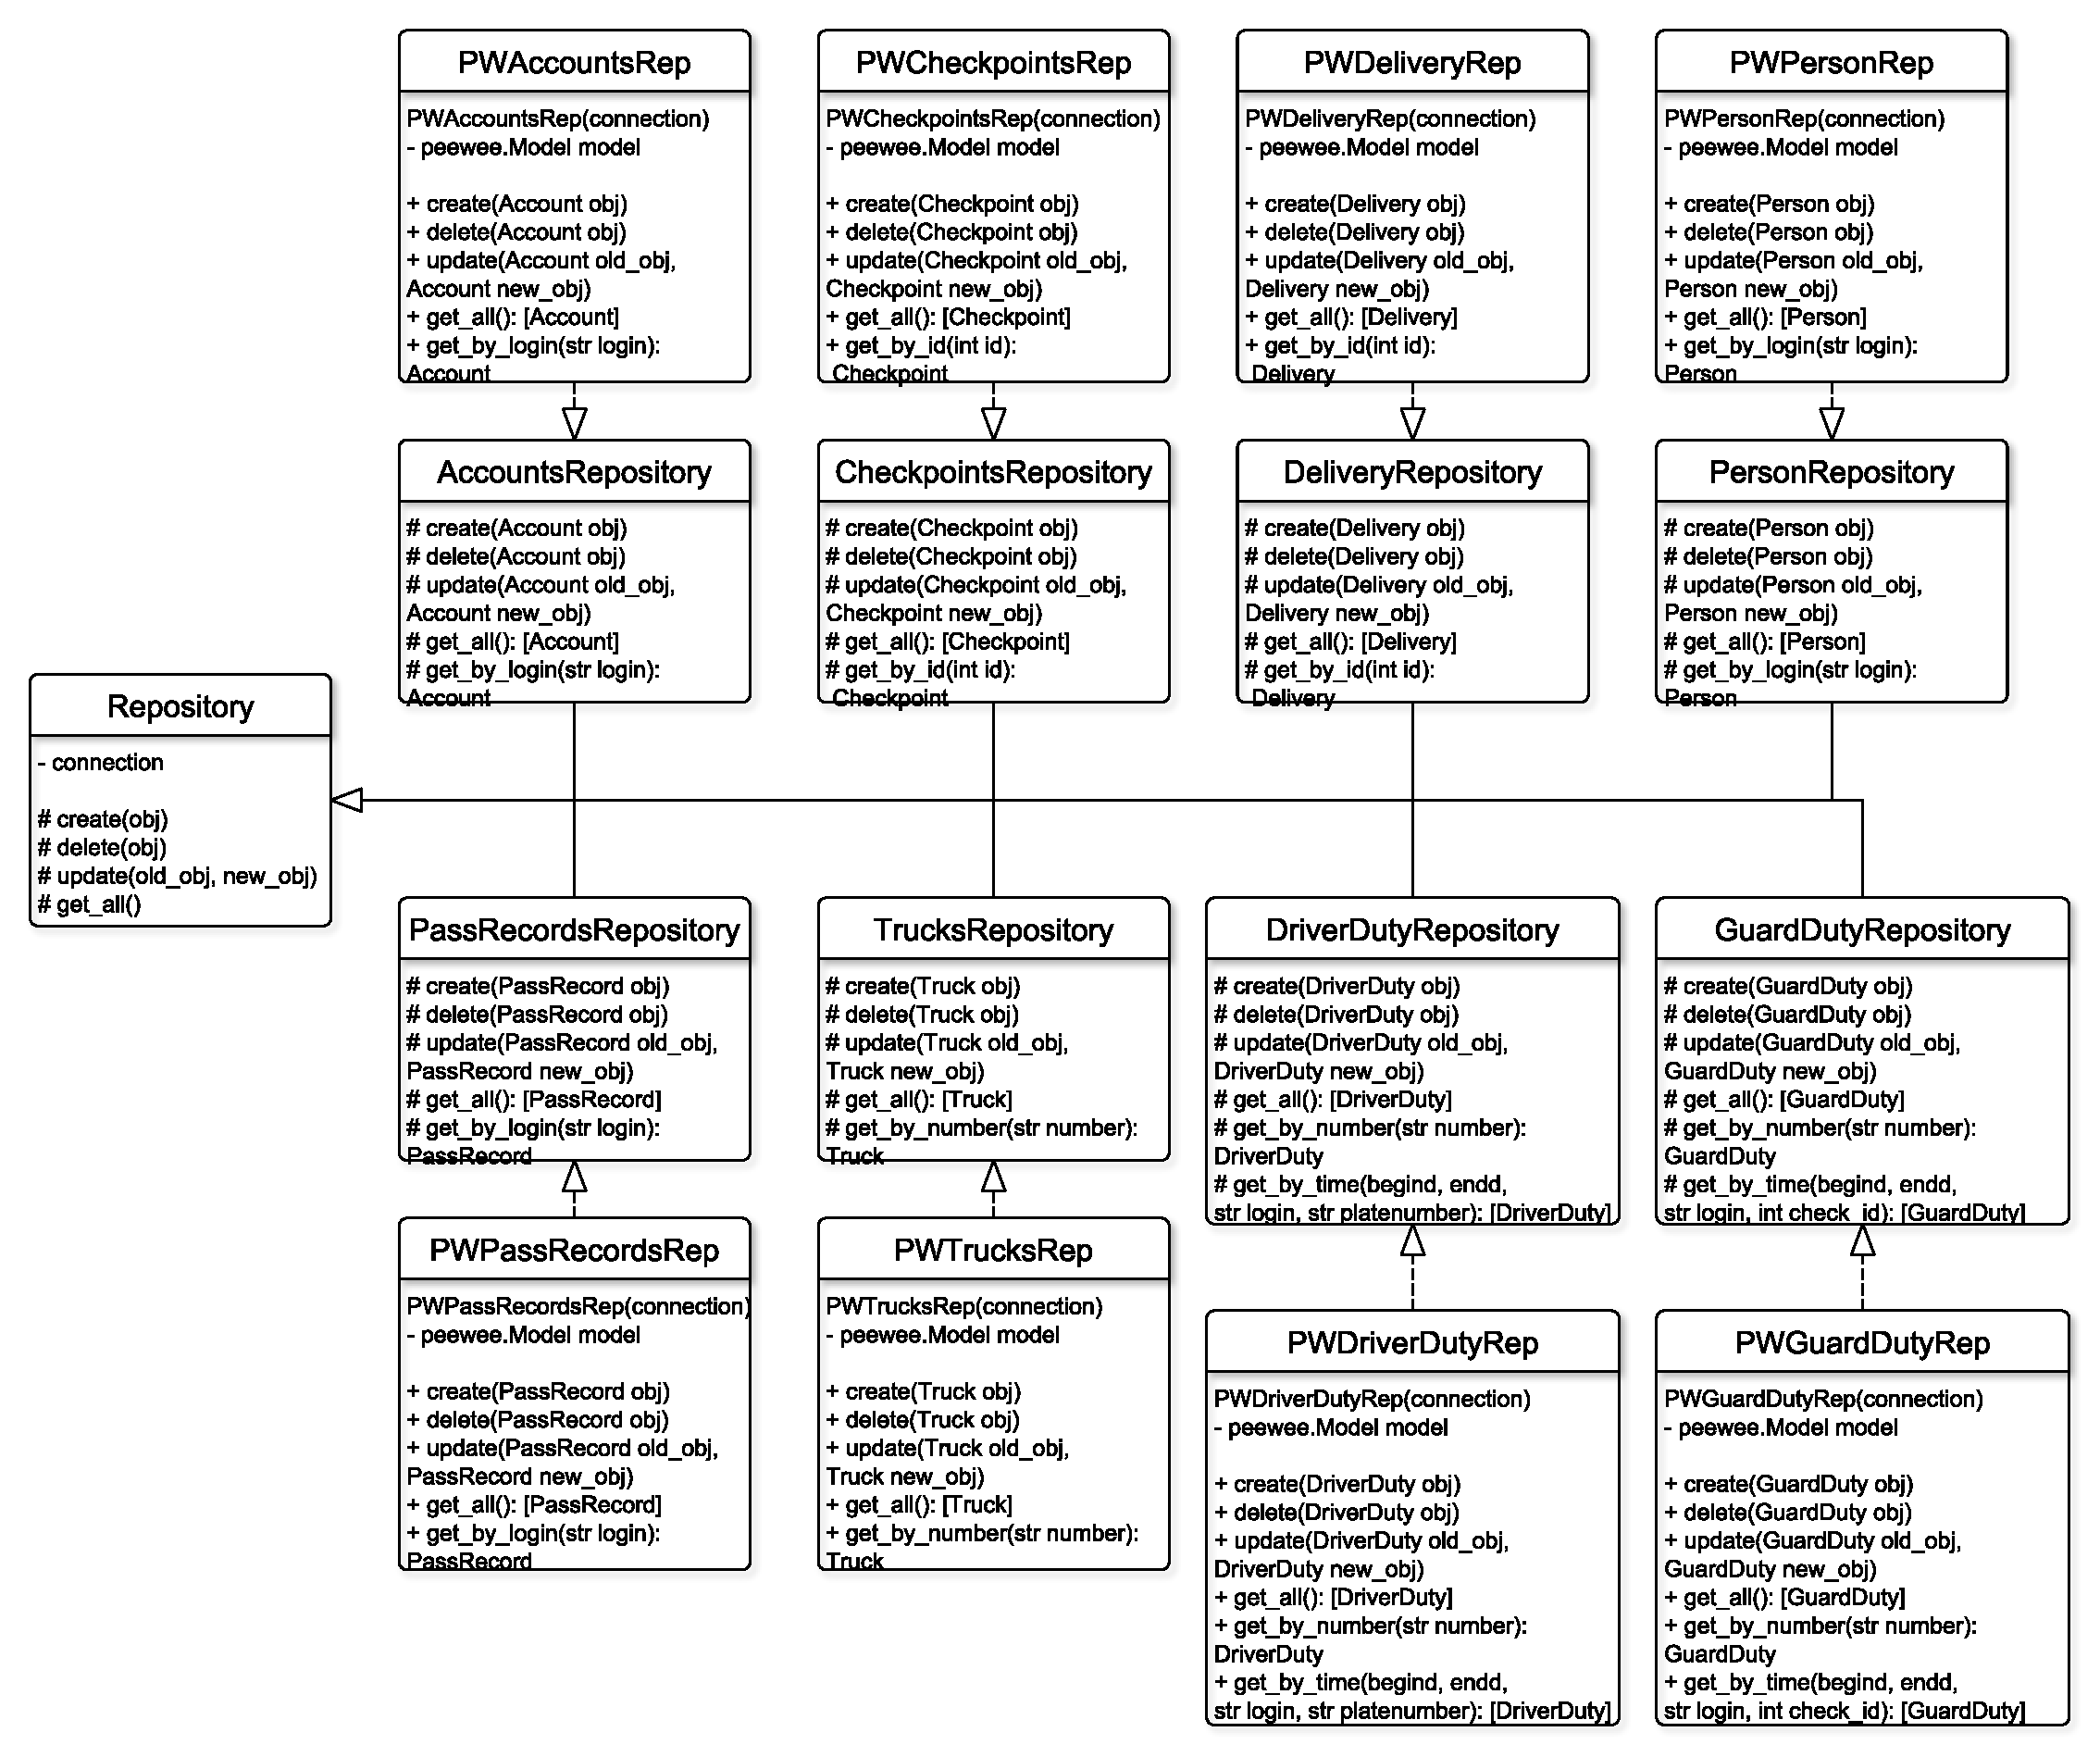
\includegraphics[scale=0.4, angle=0]{uml/repsoitory.pdf}}
		\caption{UML-диаграмма компонента доступа к данным}
	\end{center}
\end{figure}

\newpage
\subsection{Компонент бизнес-логики}
В соответствии с подходом MVC был создан компонент бизнес-логики, выполняющий основную обработку данных, UML диаграмма которого представленна на рисунке \hyperref[model_pic]{3.2}  

\begin{figure}[h!] \label{model_pic}
	\begin{center}
		%		{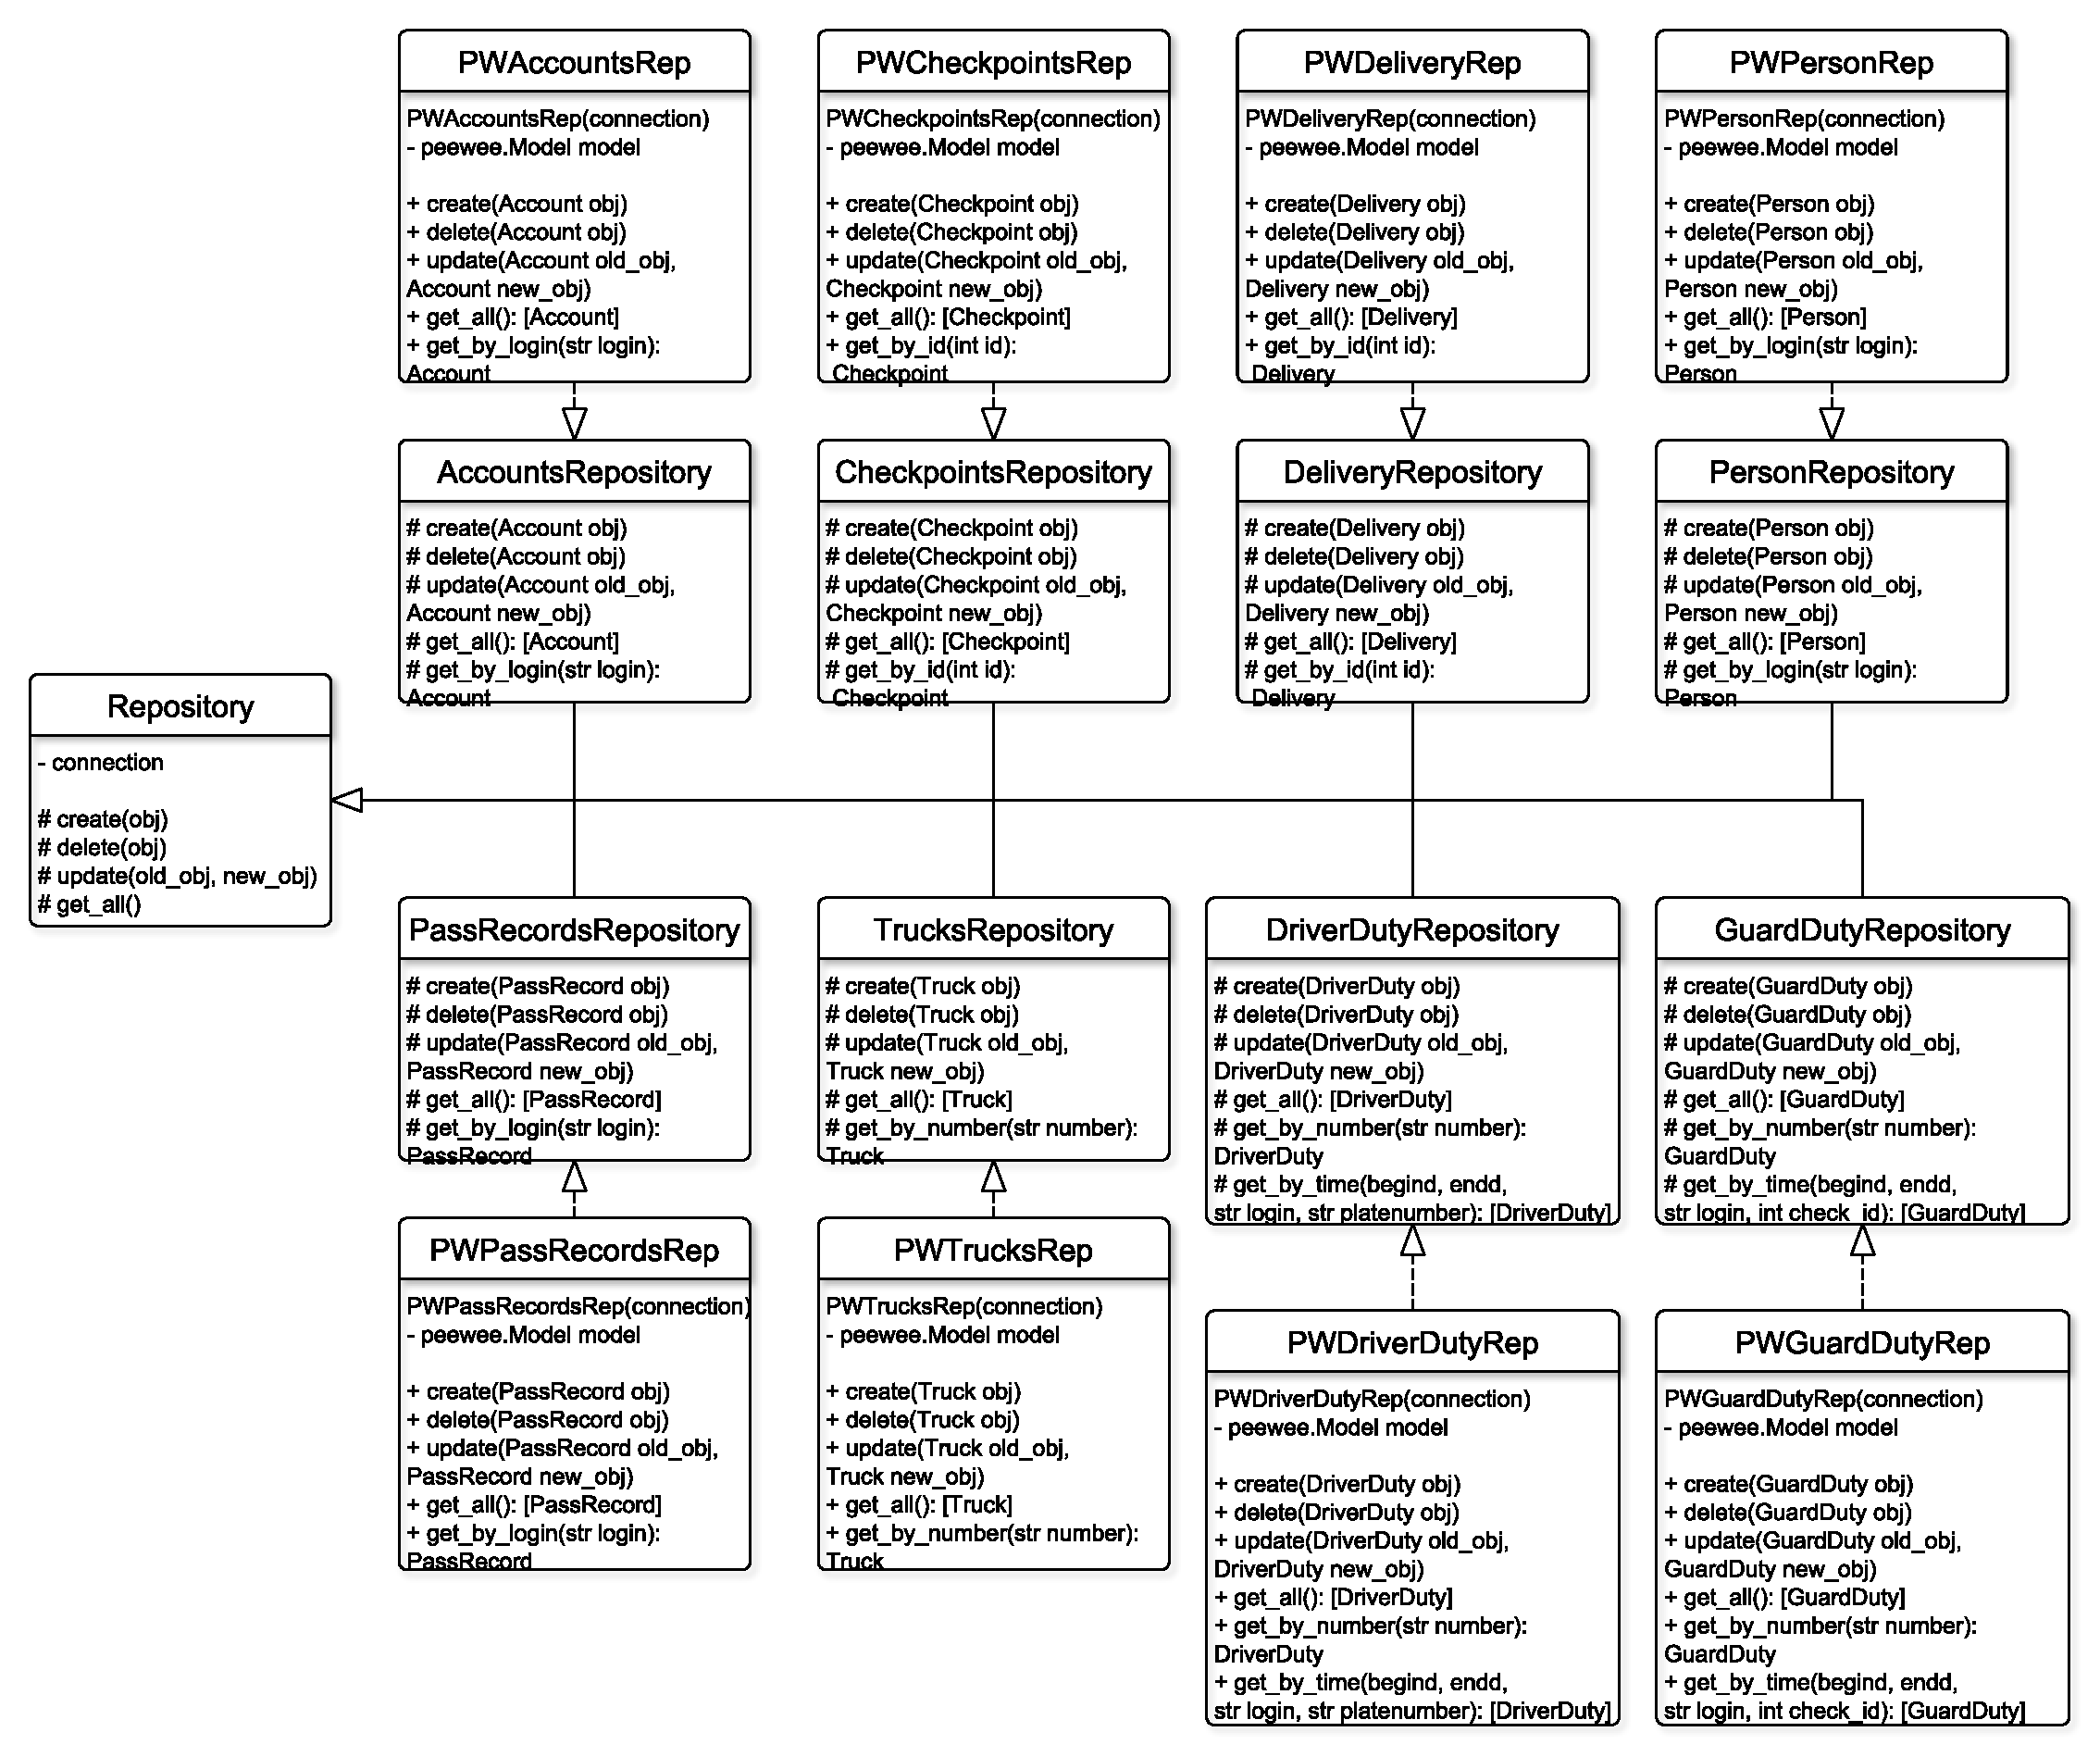
\includegraphics[height=14cm, width = 14cm]{uml/repsoitory.pdf}}
		{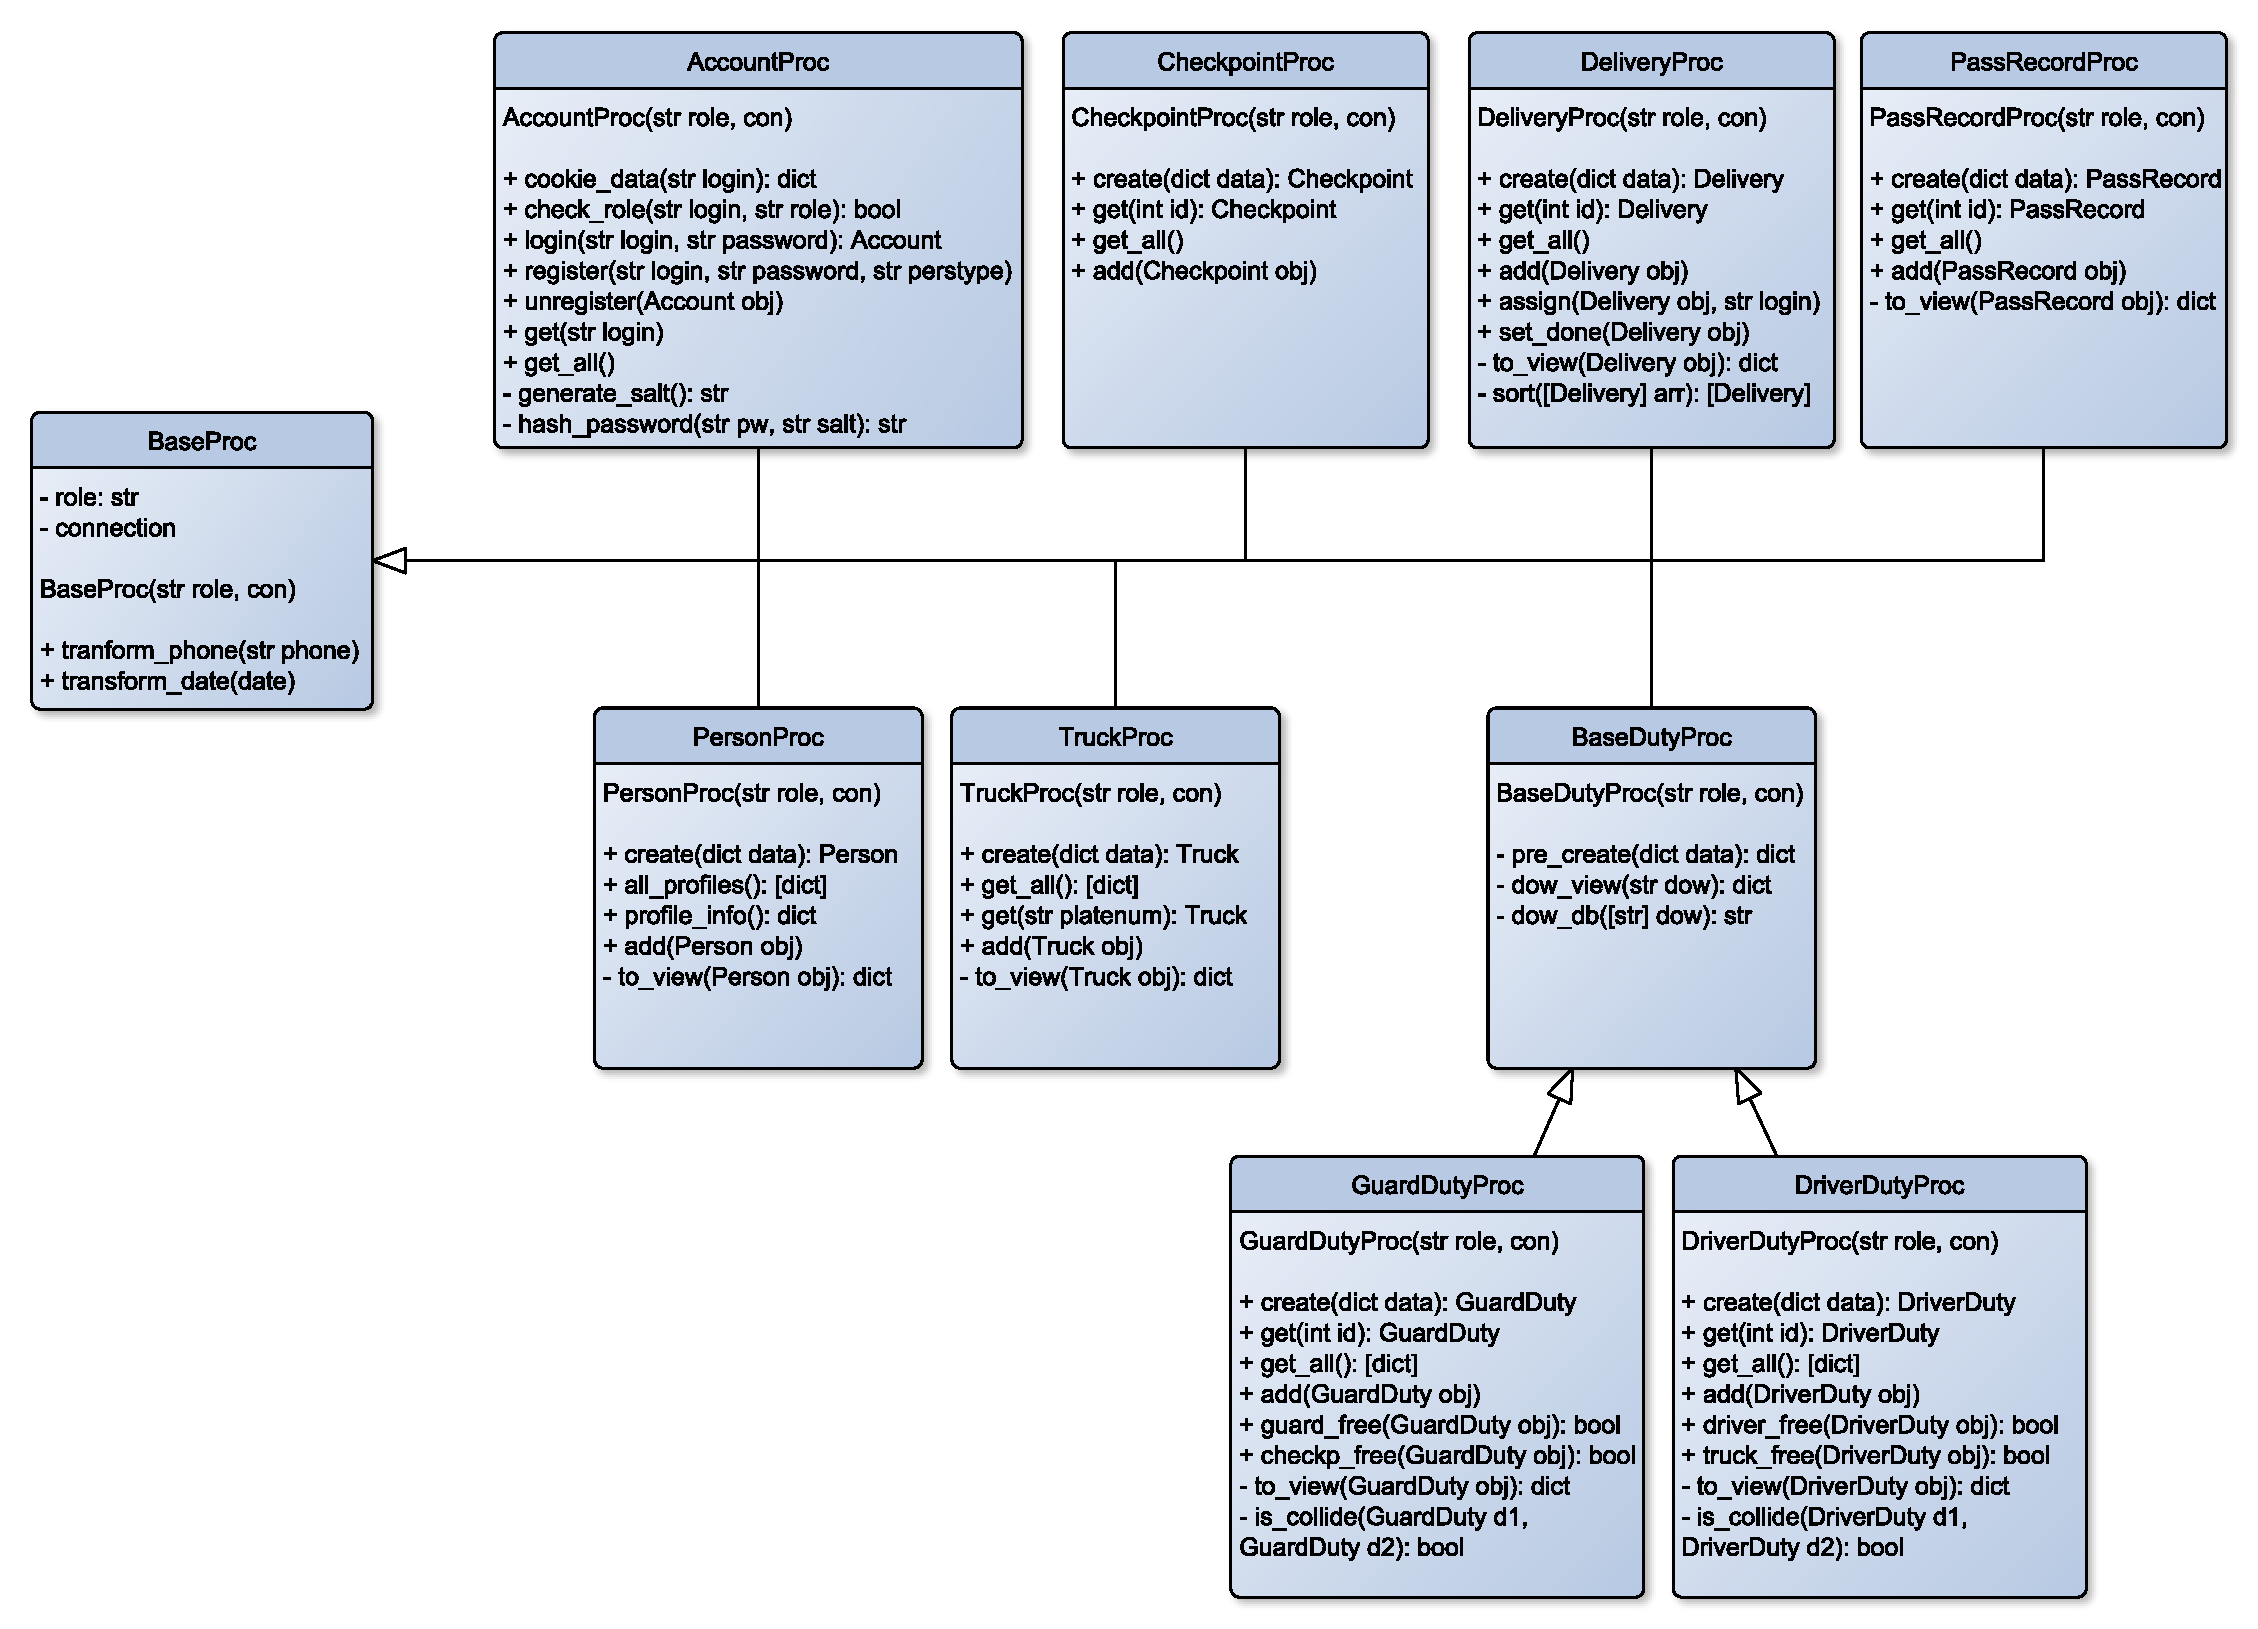
\includegraphics[scale=0.5, angle=0]{uml/business_models.pdf}}
		\caption{UML-диаграмма компонента бизнес-логики}
	\end{center}
\end{figure}

\newpage
\subsection{Компонент представления}
Также создан компонент представления, выполняющий отображение web-страниц в ответ на запросы пользователя, UML диаграмма которого представленна на рисунке \hyperref[view_pic]{3.3}. Помимо этого был реализован технический компонент представления, отображающий информацию в символьном виде, для возможности тестирования компонента бизнес-логики.

\begin{figure}[h!] \label{view_pic}
	\begin{center}
		%		{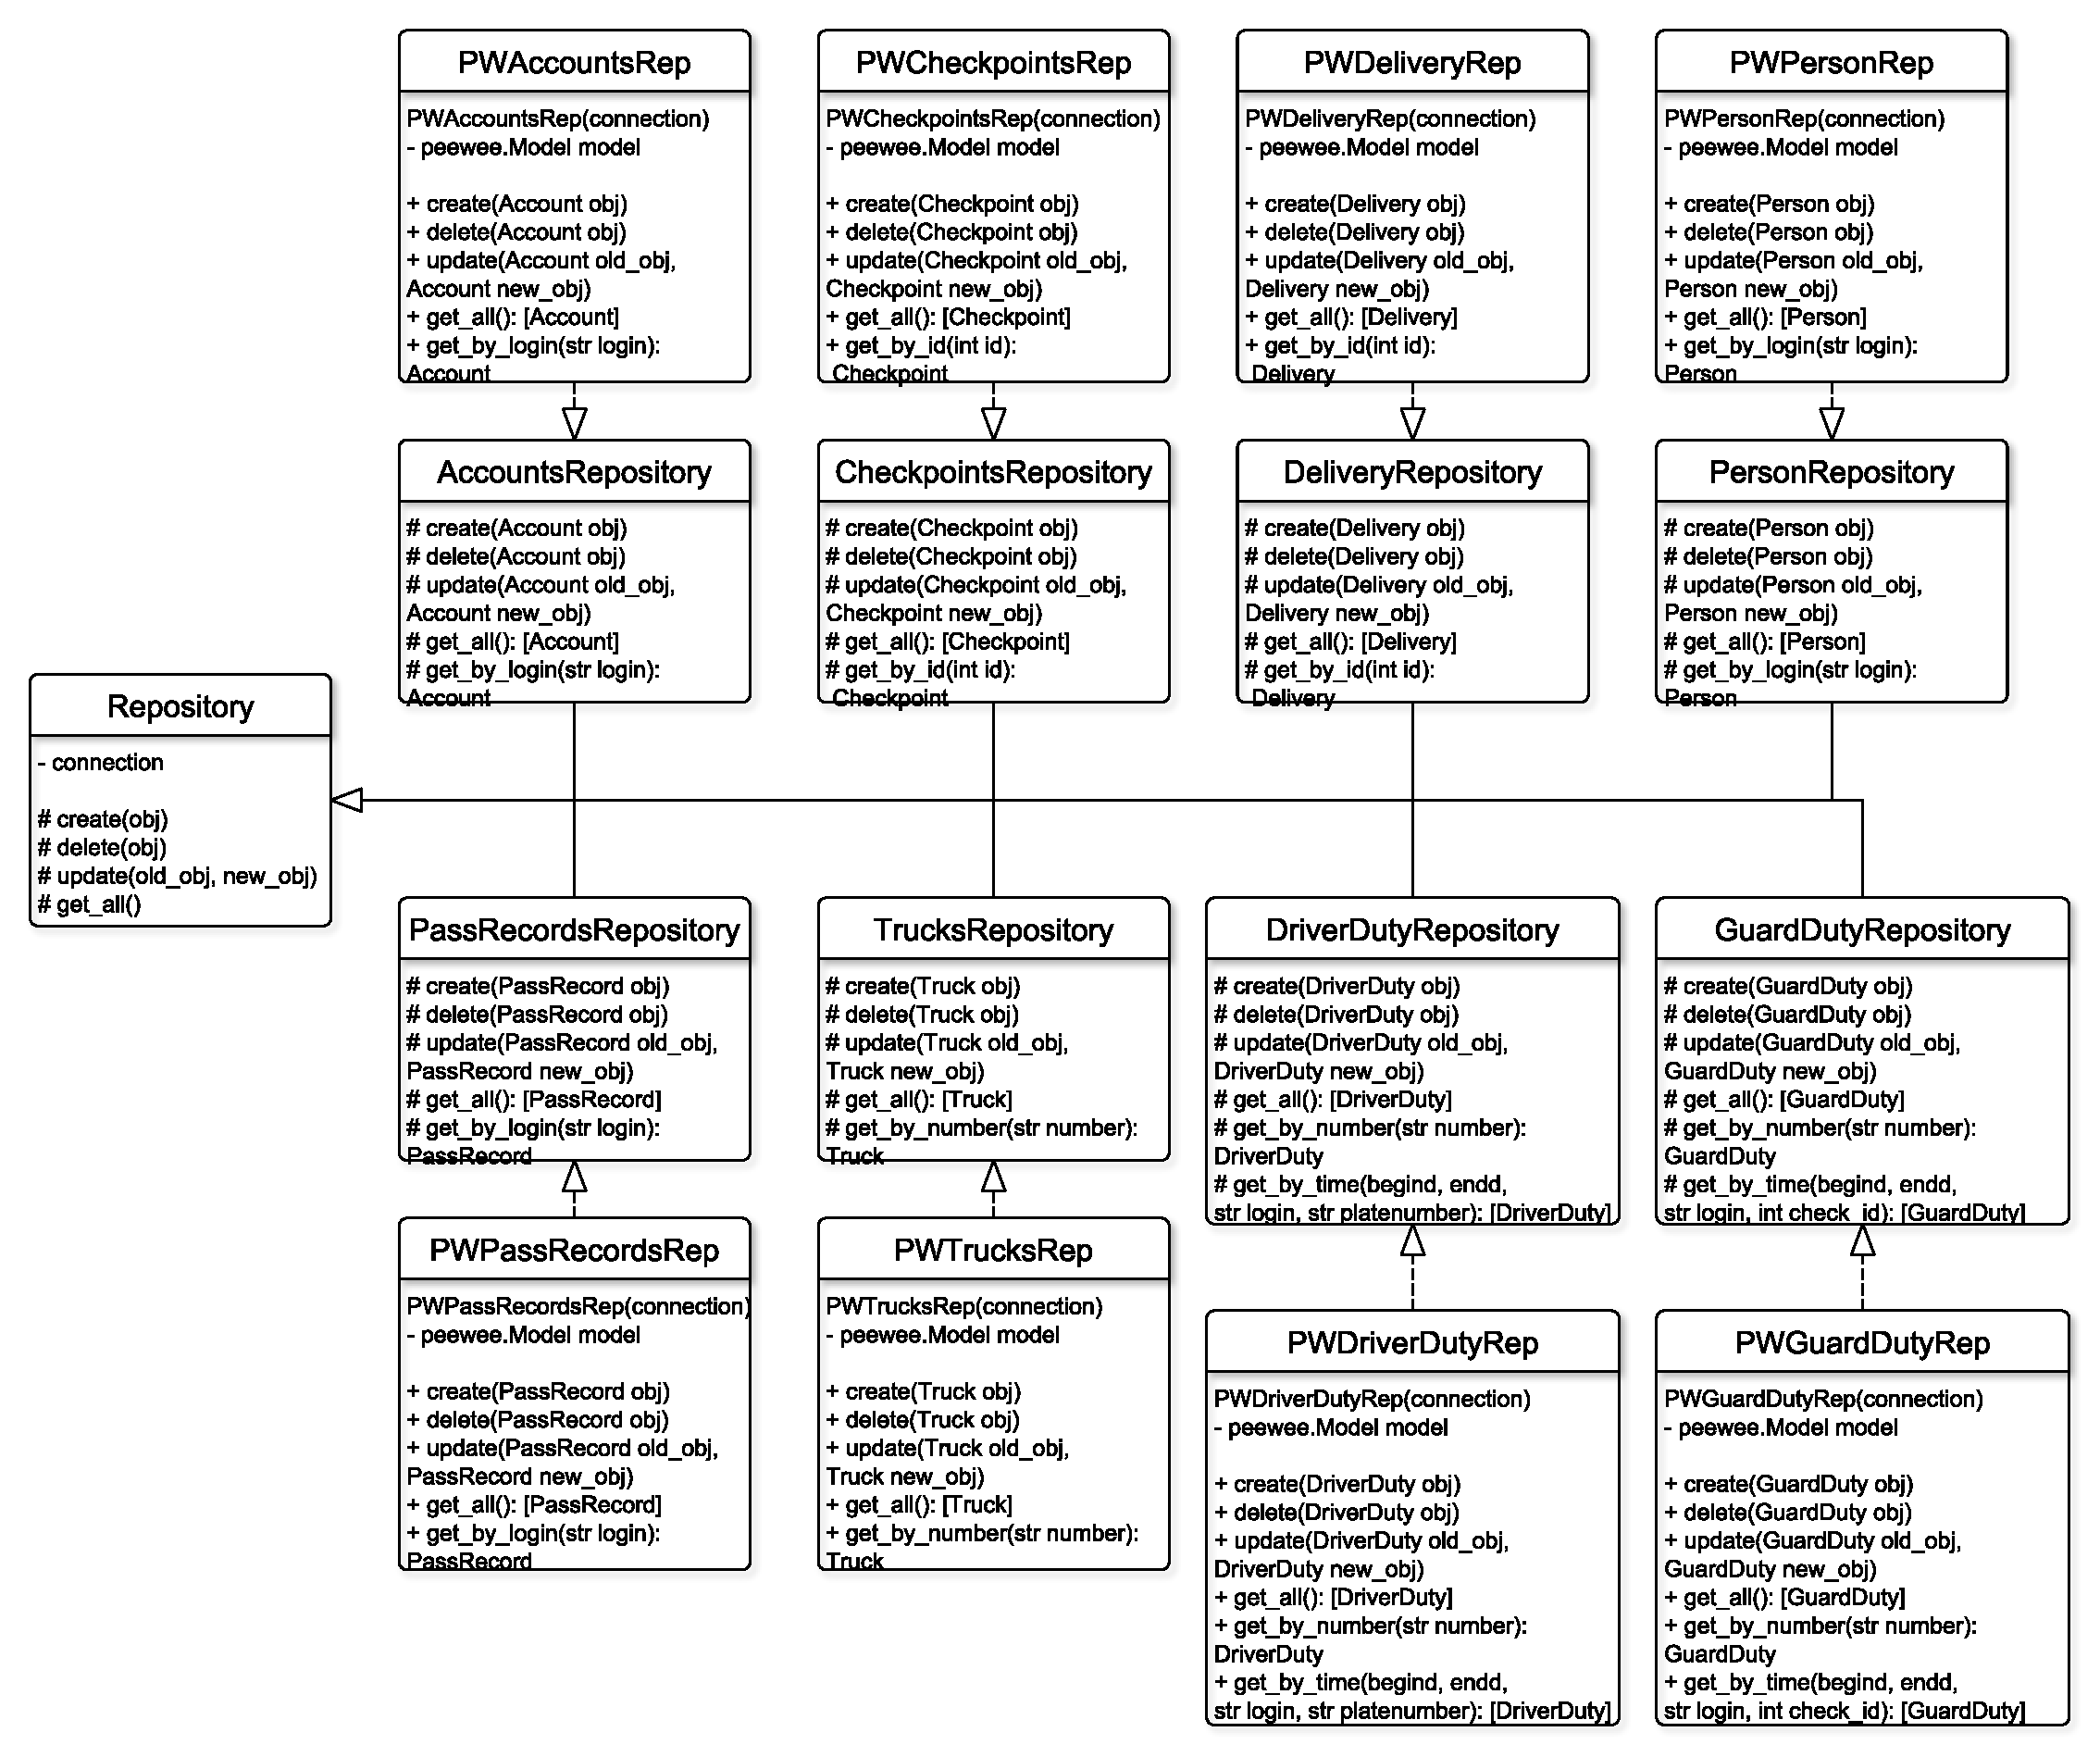
\includegraphics[height=14cm, width = 14cm]{uml/repsoitory.pdf}}
		{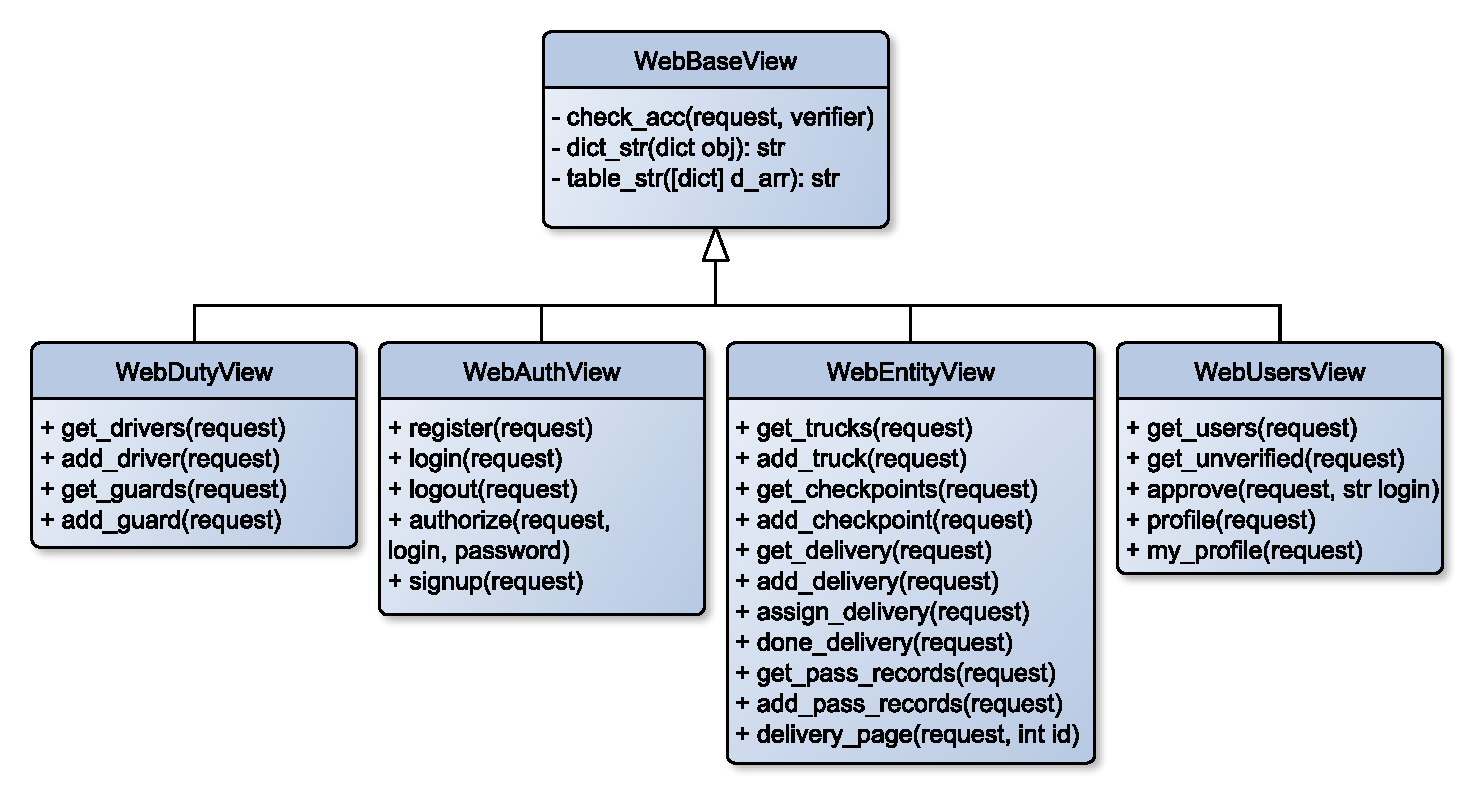
\includegraphics[scale=0.5, angle=0]{uml/webGUI.pdf}}
		\caption{UML-диаграмма компонента web-представления}
	\end{center}
\end{figure}

\newpage
\subsection{Диаграмма приложения}
Все перечисленные компоненты можно объединить в одну UML-диаграмму всего приложения на рисунке \hyperref[alluml_pic]{3.4}

\begin{figure}[h!] \label{alluml_pic}
	\begin{center}
		%		{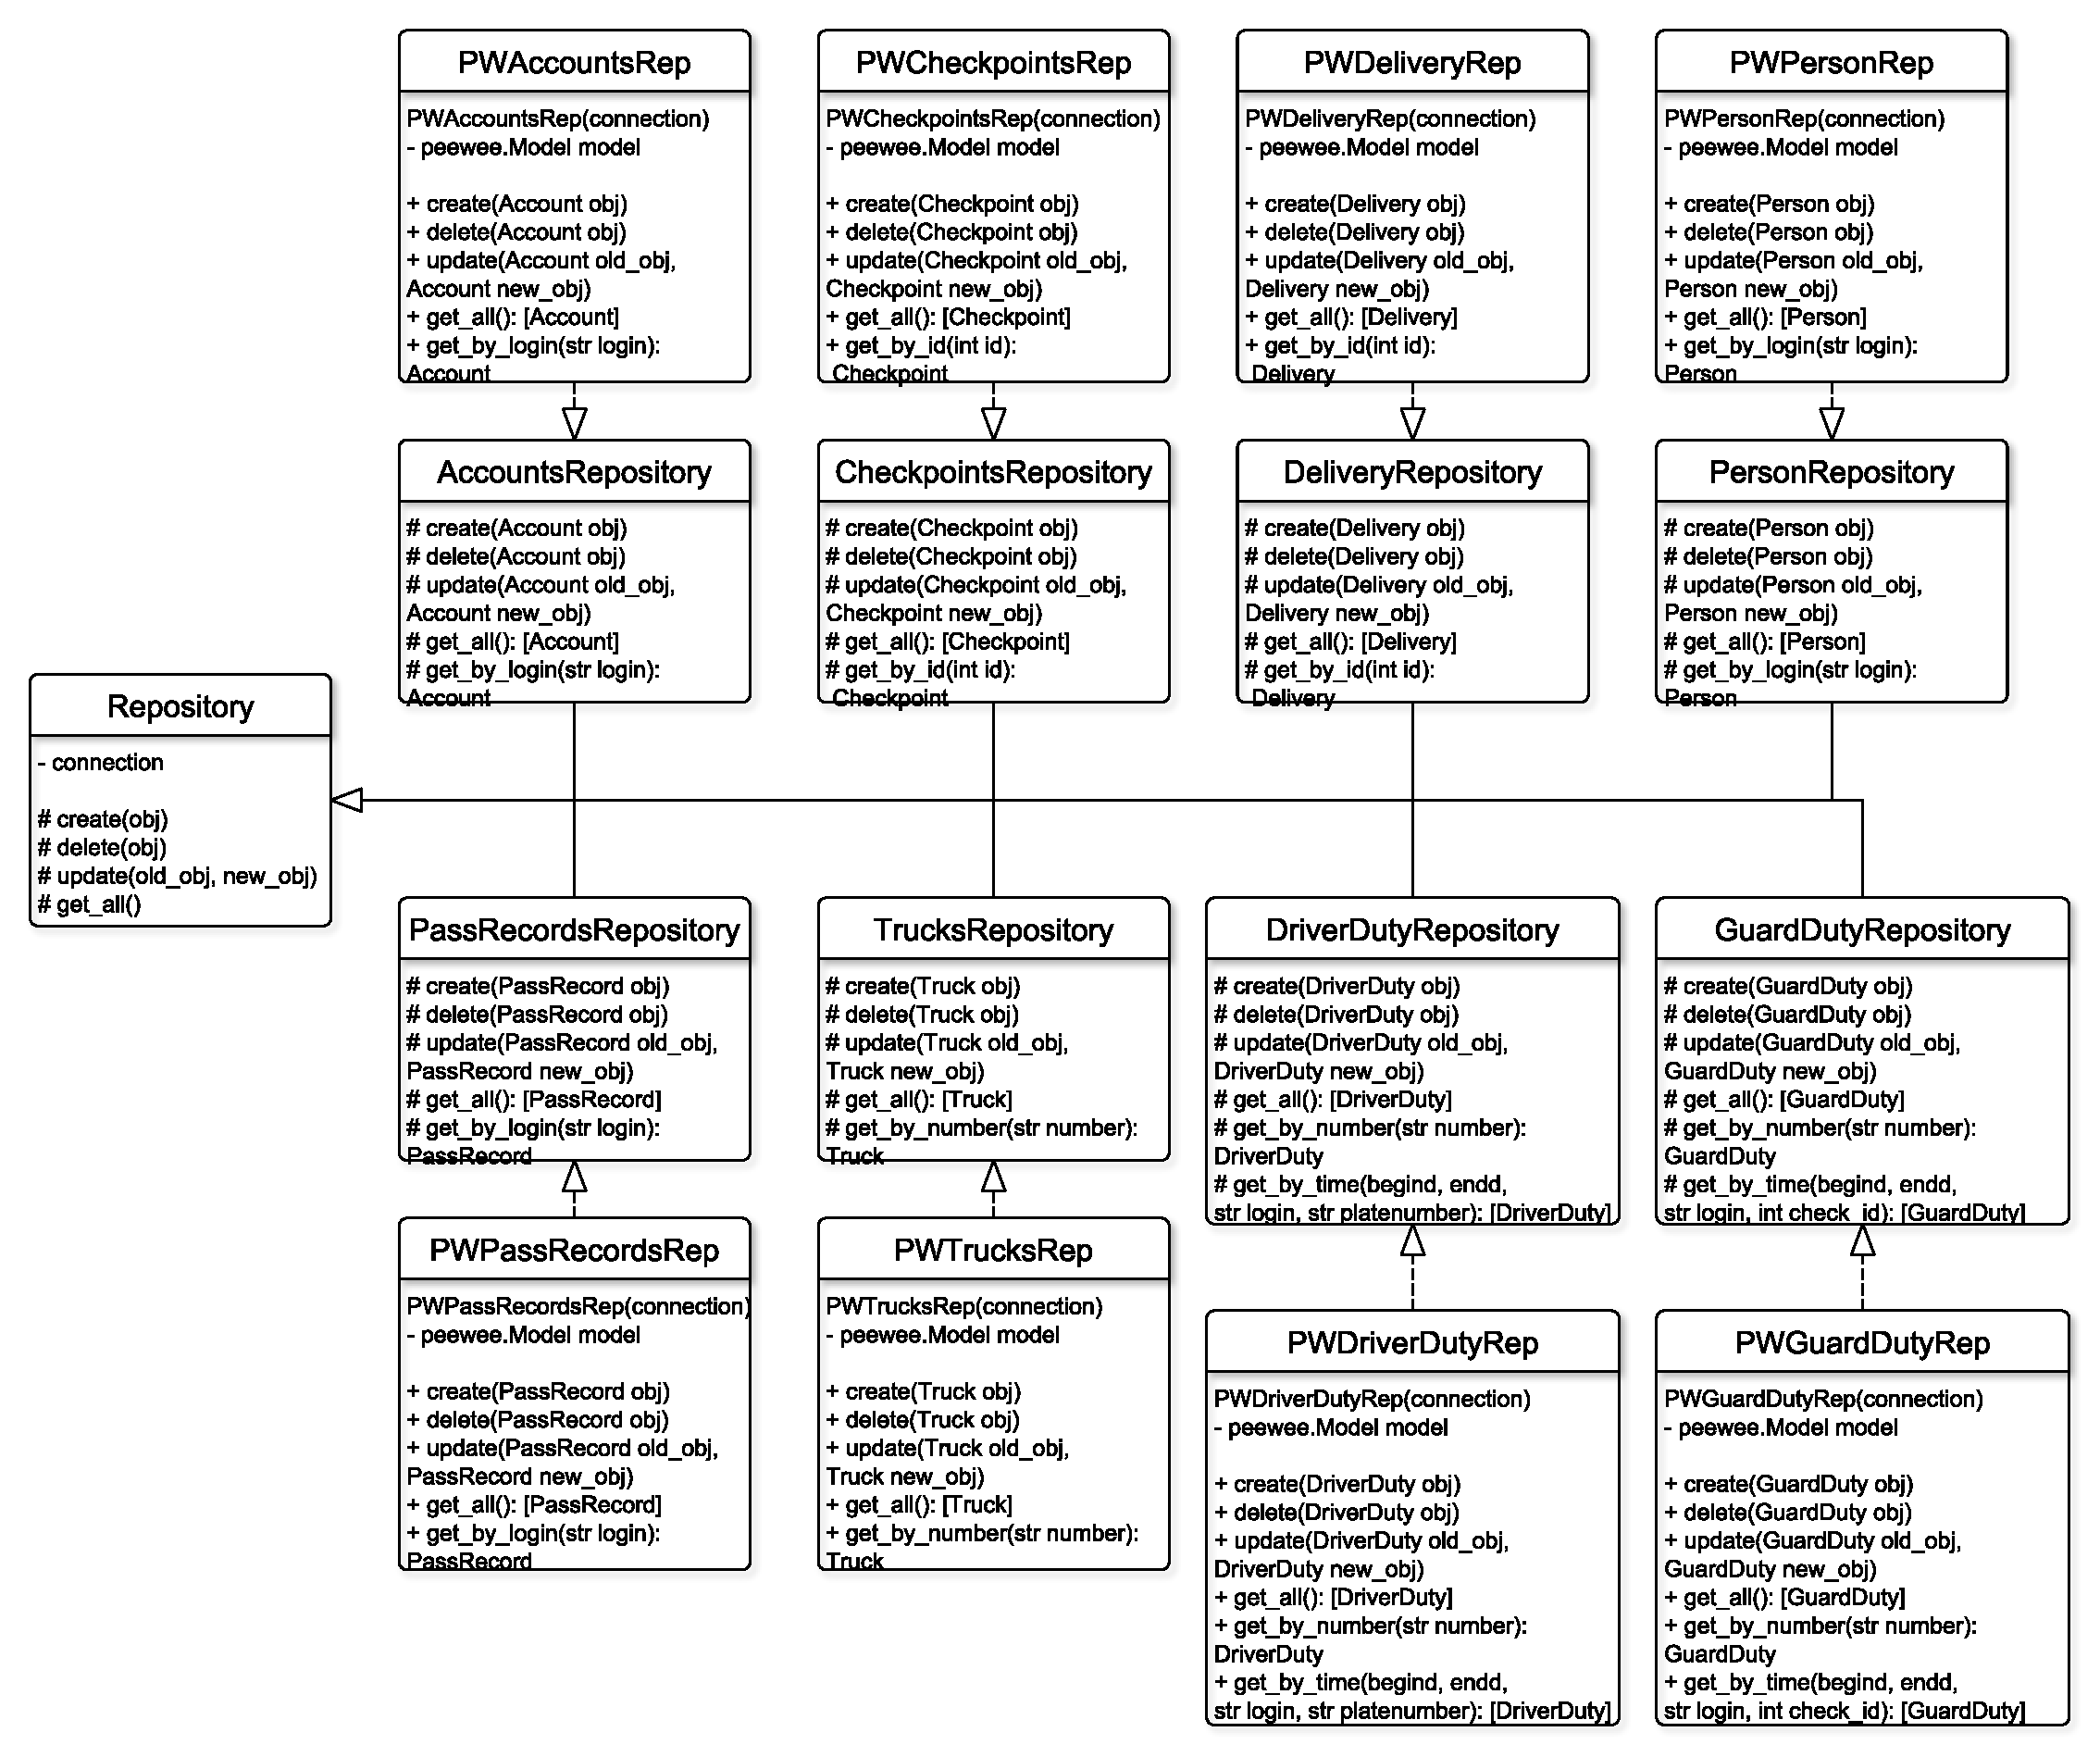
\includegraphics[height=14cm, width = 14cm]{uml/repsoitory.pdf}}
		{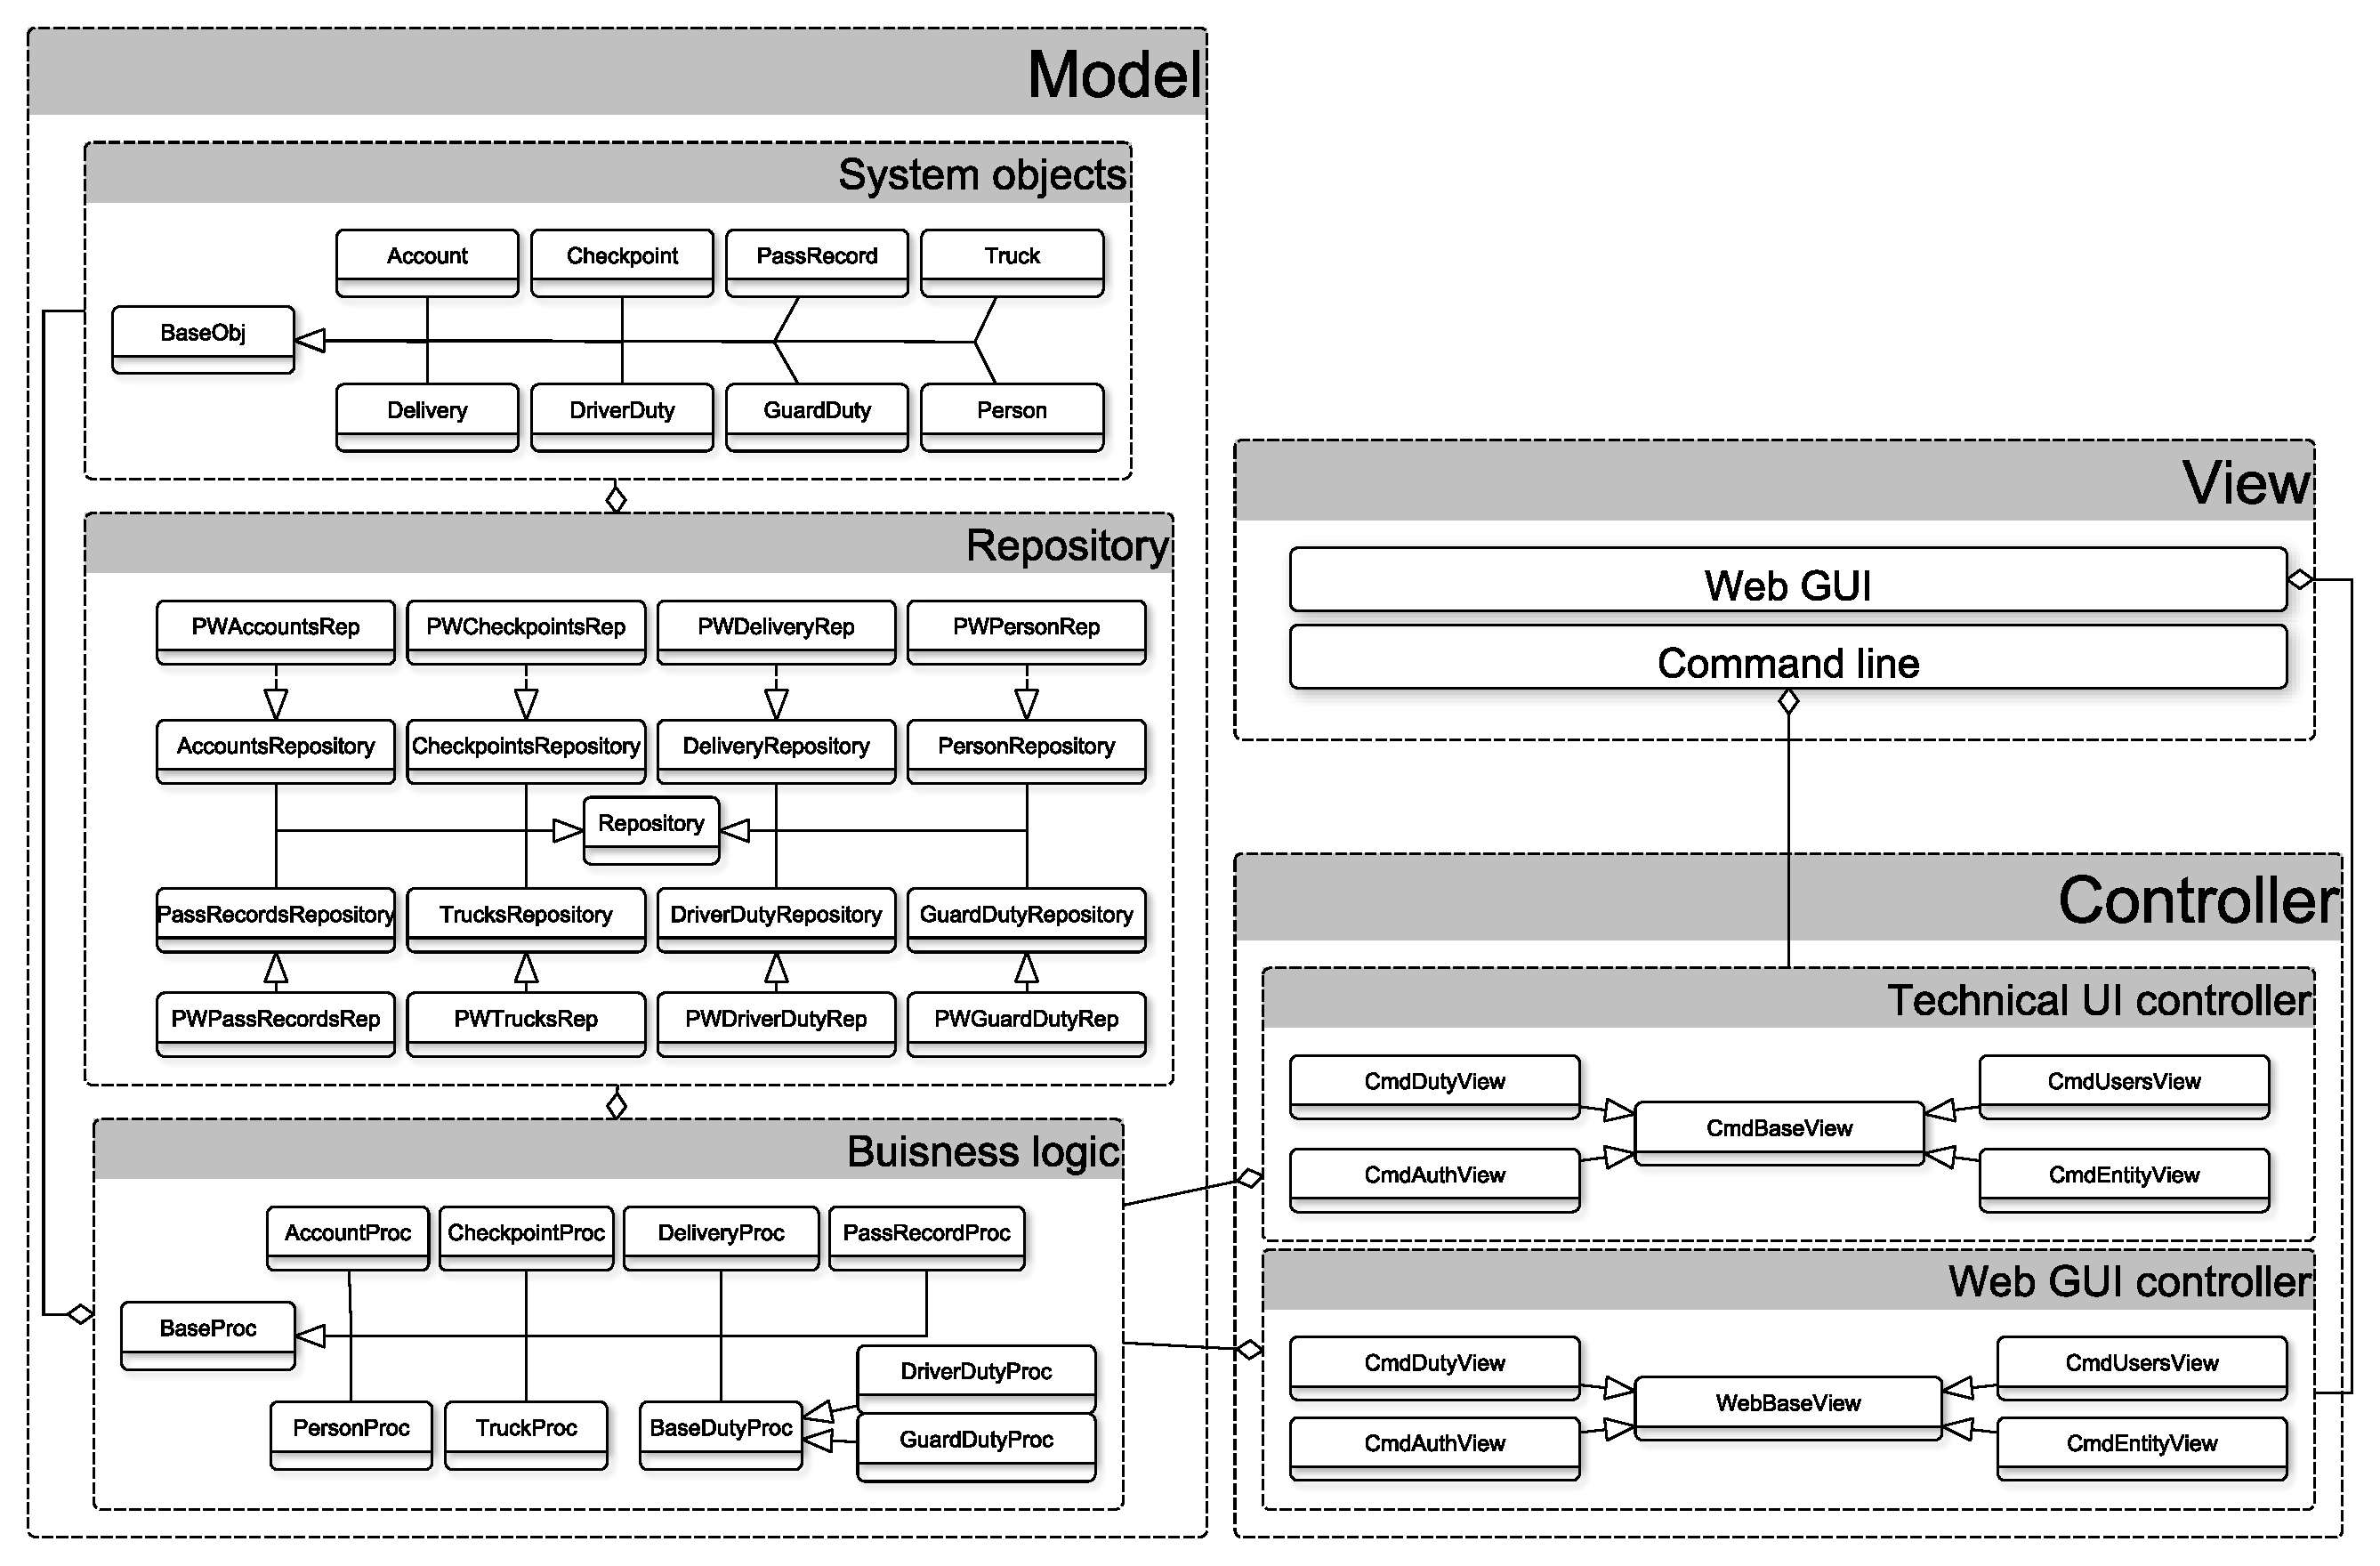
\includegraphics[scale=0.36, angle=-90]{uml/components.pdf}}
		\caption{UML-диаграмма компонента web-представления}
	\end{center}
\end{figure}


\section{Интерфейс приложения}
Для авторизованного пользователя в заголовке каждой страницы содержится панель навигации, предоставляющая возможность перейти на все страницы, функционально соответствующие его роли. Данная панель изображена на примере администратора на рисунке \hyperref[navbar_sc]{3.5}. Некоторые пункты меню являются выпадающими, их можно открыть наведением мыши. Также в левом углу панели присутствует элемент информационного или ошибочного сообщения.

На рисунках \hyperref[navbar_sc]{3.5}-\hyperref[trucks_sc]{3.11} приведена демонстрация ключевых страниц для роли администратора. На рисунках \hyperref[pick_delivery_sc]{3.12}, \hyperref[driver_profile_sc]{3.13} и \hyperref[guard_duty_sc]{3.14}, \hyperref[guard_duty_sc]{3.15} приведены страницы, уникальные для ролей водителя и охранника соотвественно.

\begin{figure}[h!] \label{navbar_sc}
	\begin{center}
		%		{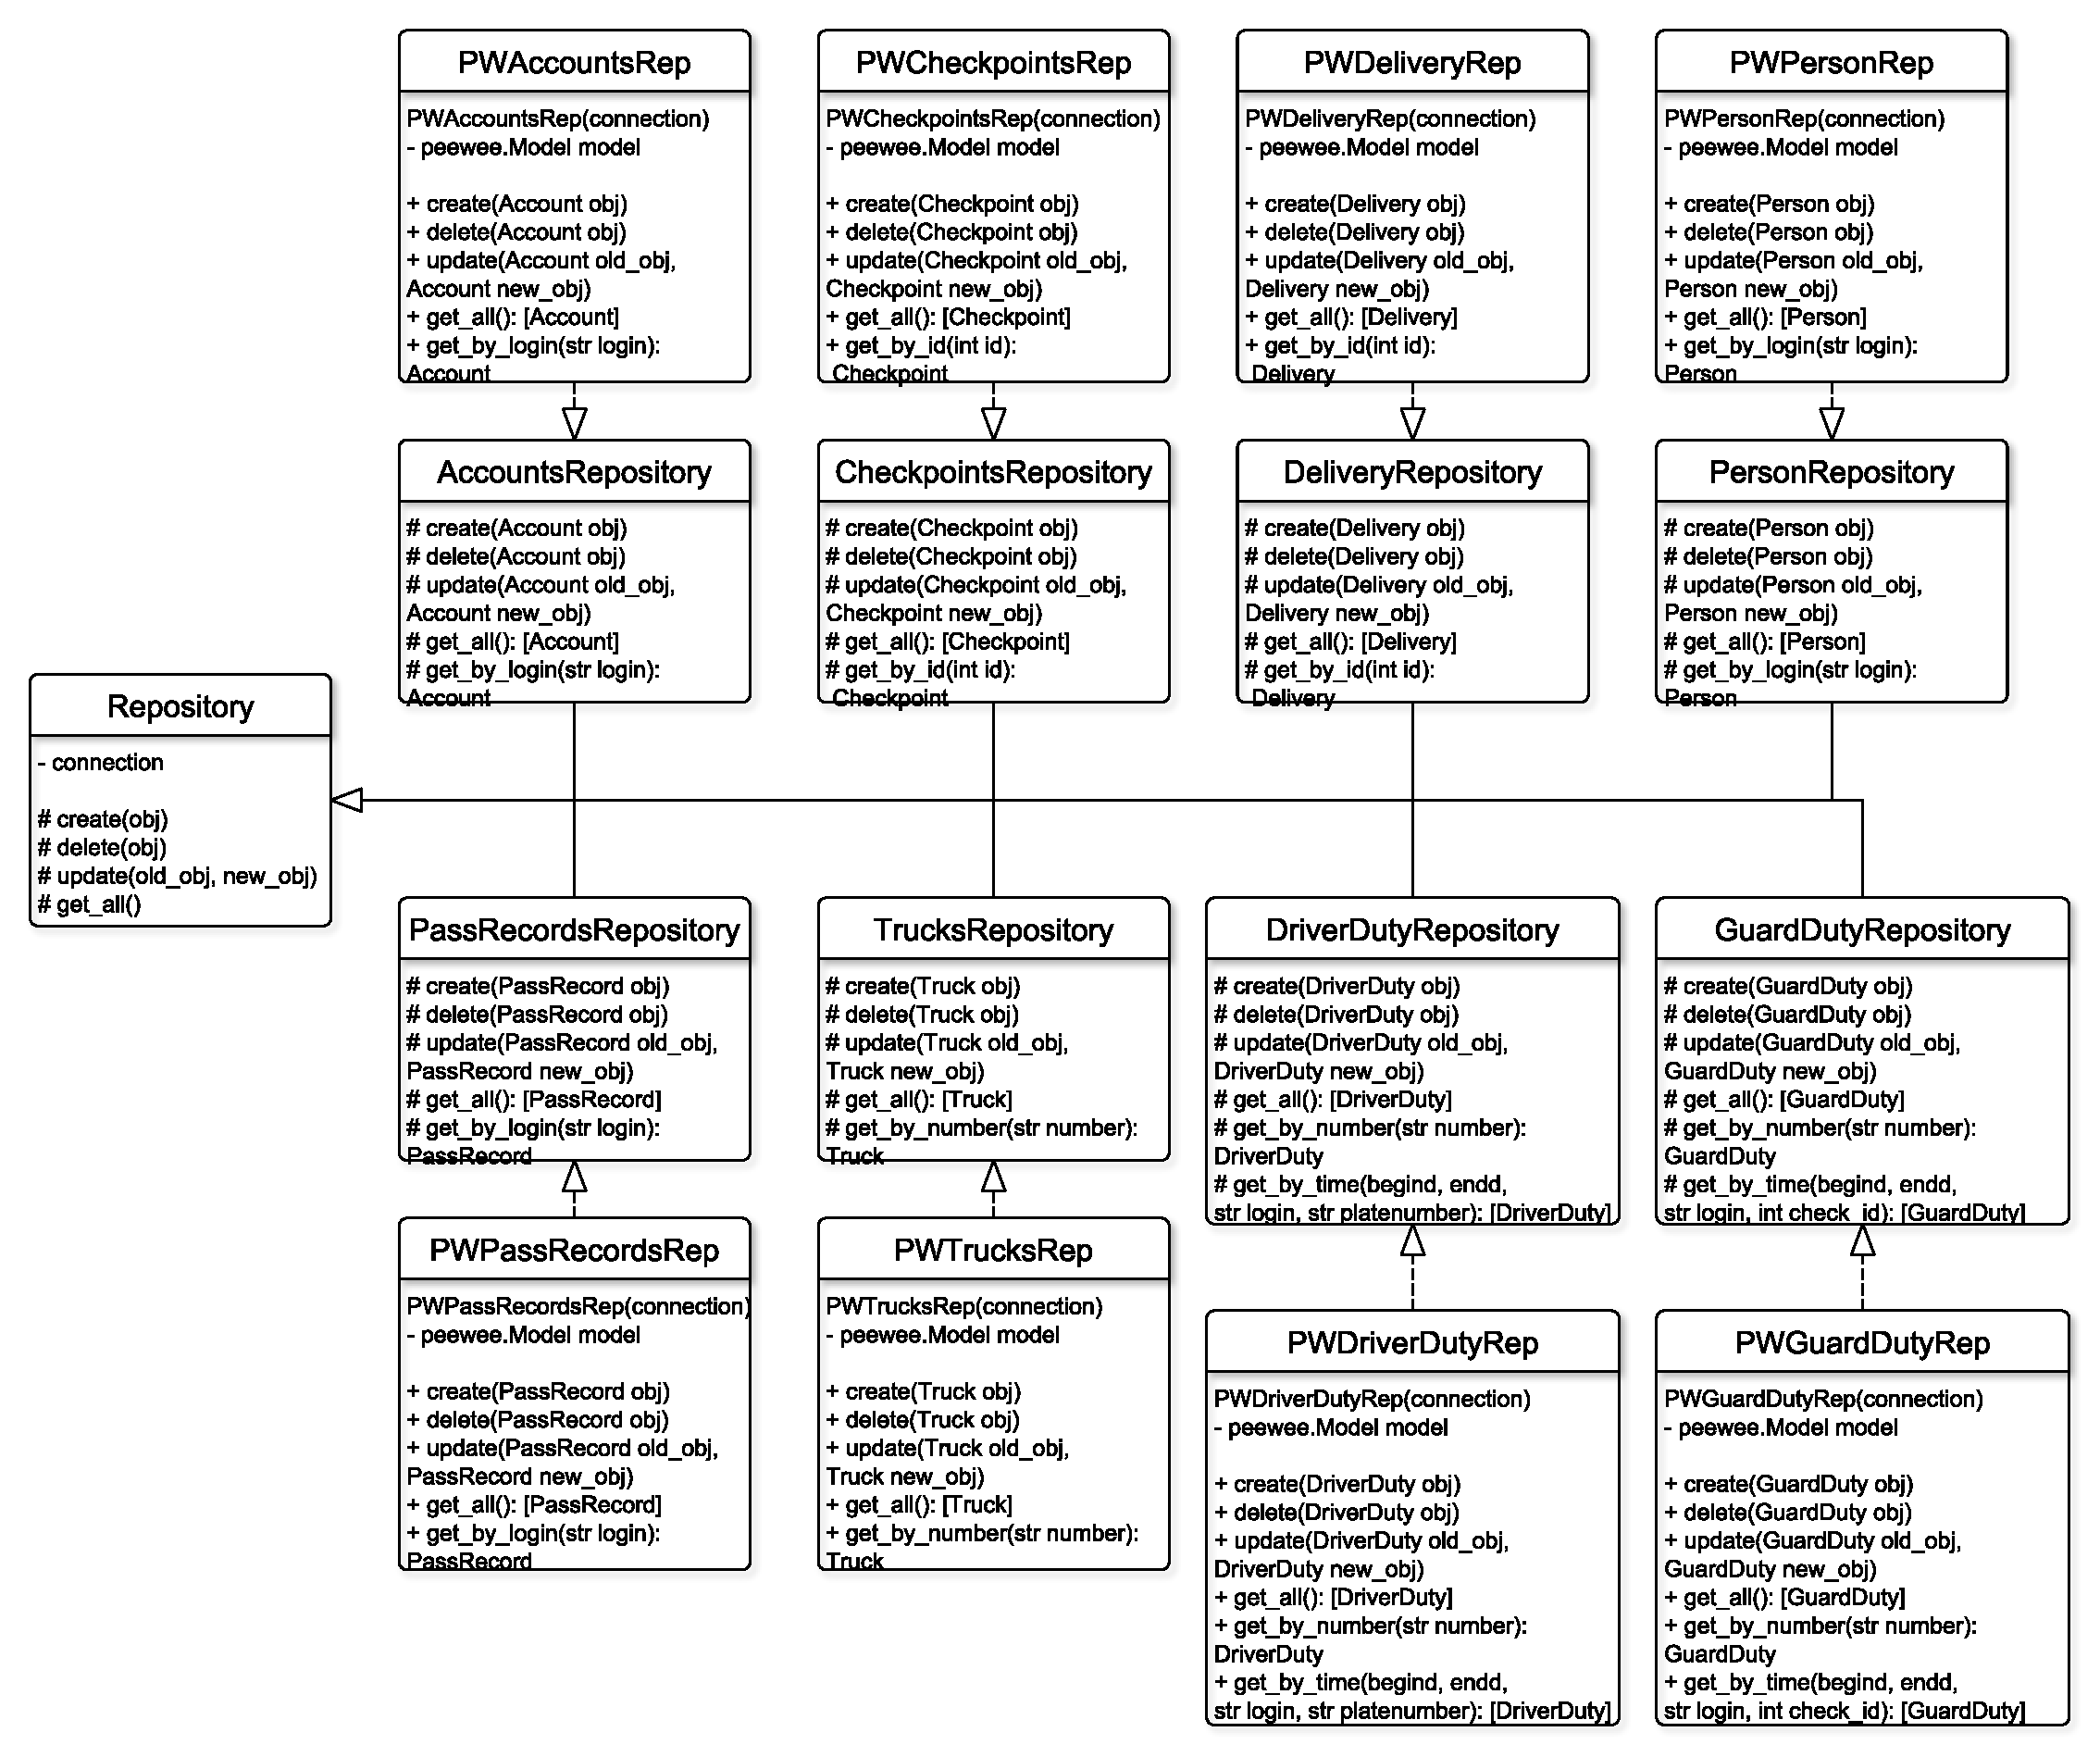
\includegraphics[height=14cm, width = 14cm]{uml/repsoitory.pdf}}
		{\includegraphics[scale=0.45, angle=0]{sc/admin_profile}}
		\caption{Страница профиля администратора}
	\end{center}
\end{figure}

\begin{figure}[h!] \label{all_profiles_sc}
	\begin{center}
		%		{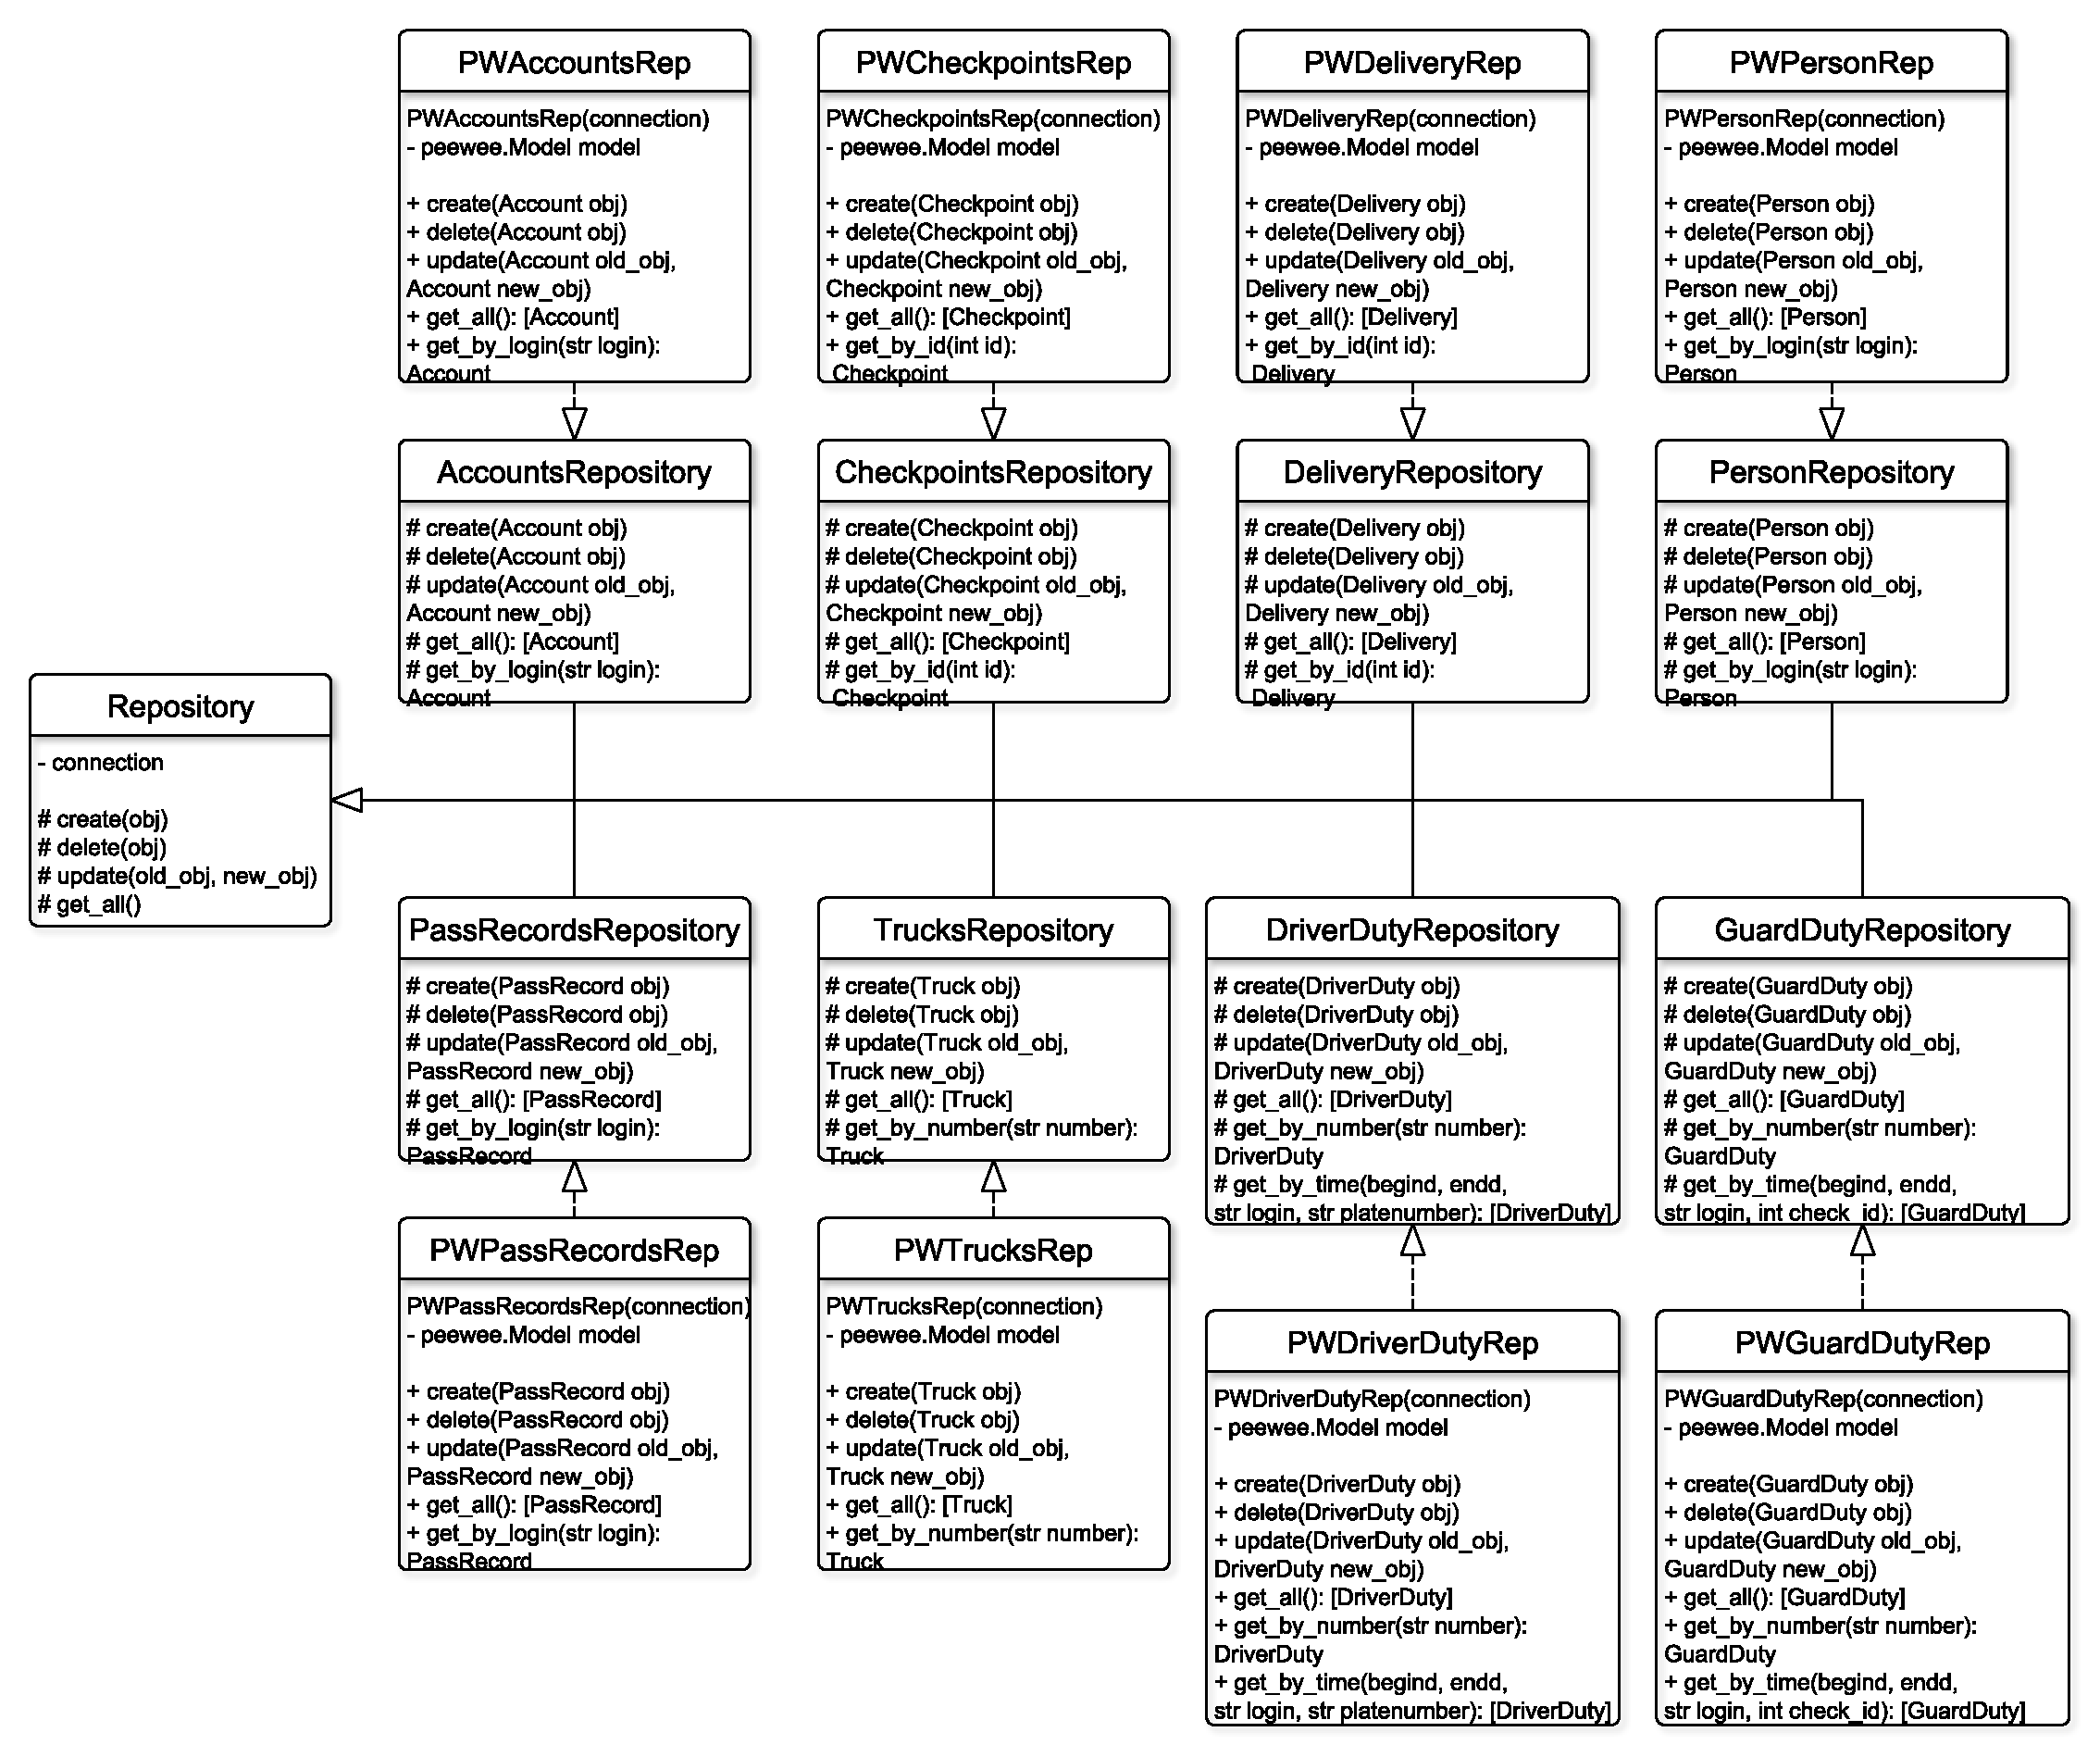
\includegraphics[height=14cm, width = 14cm]{uml/repsoitory.pdf}}
		{\includegraphics[scale=0.43, angle=0]{sc/all_profiles}}
		\caption{Страница просмотра всех сотрудников}
	\end{center}
\end{figure}

\begin{figure}[h!] \label{unver_sc}
	\begin{center}
		%		{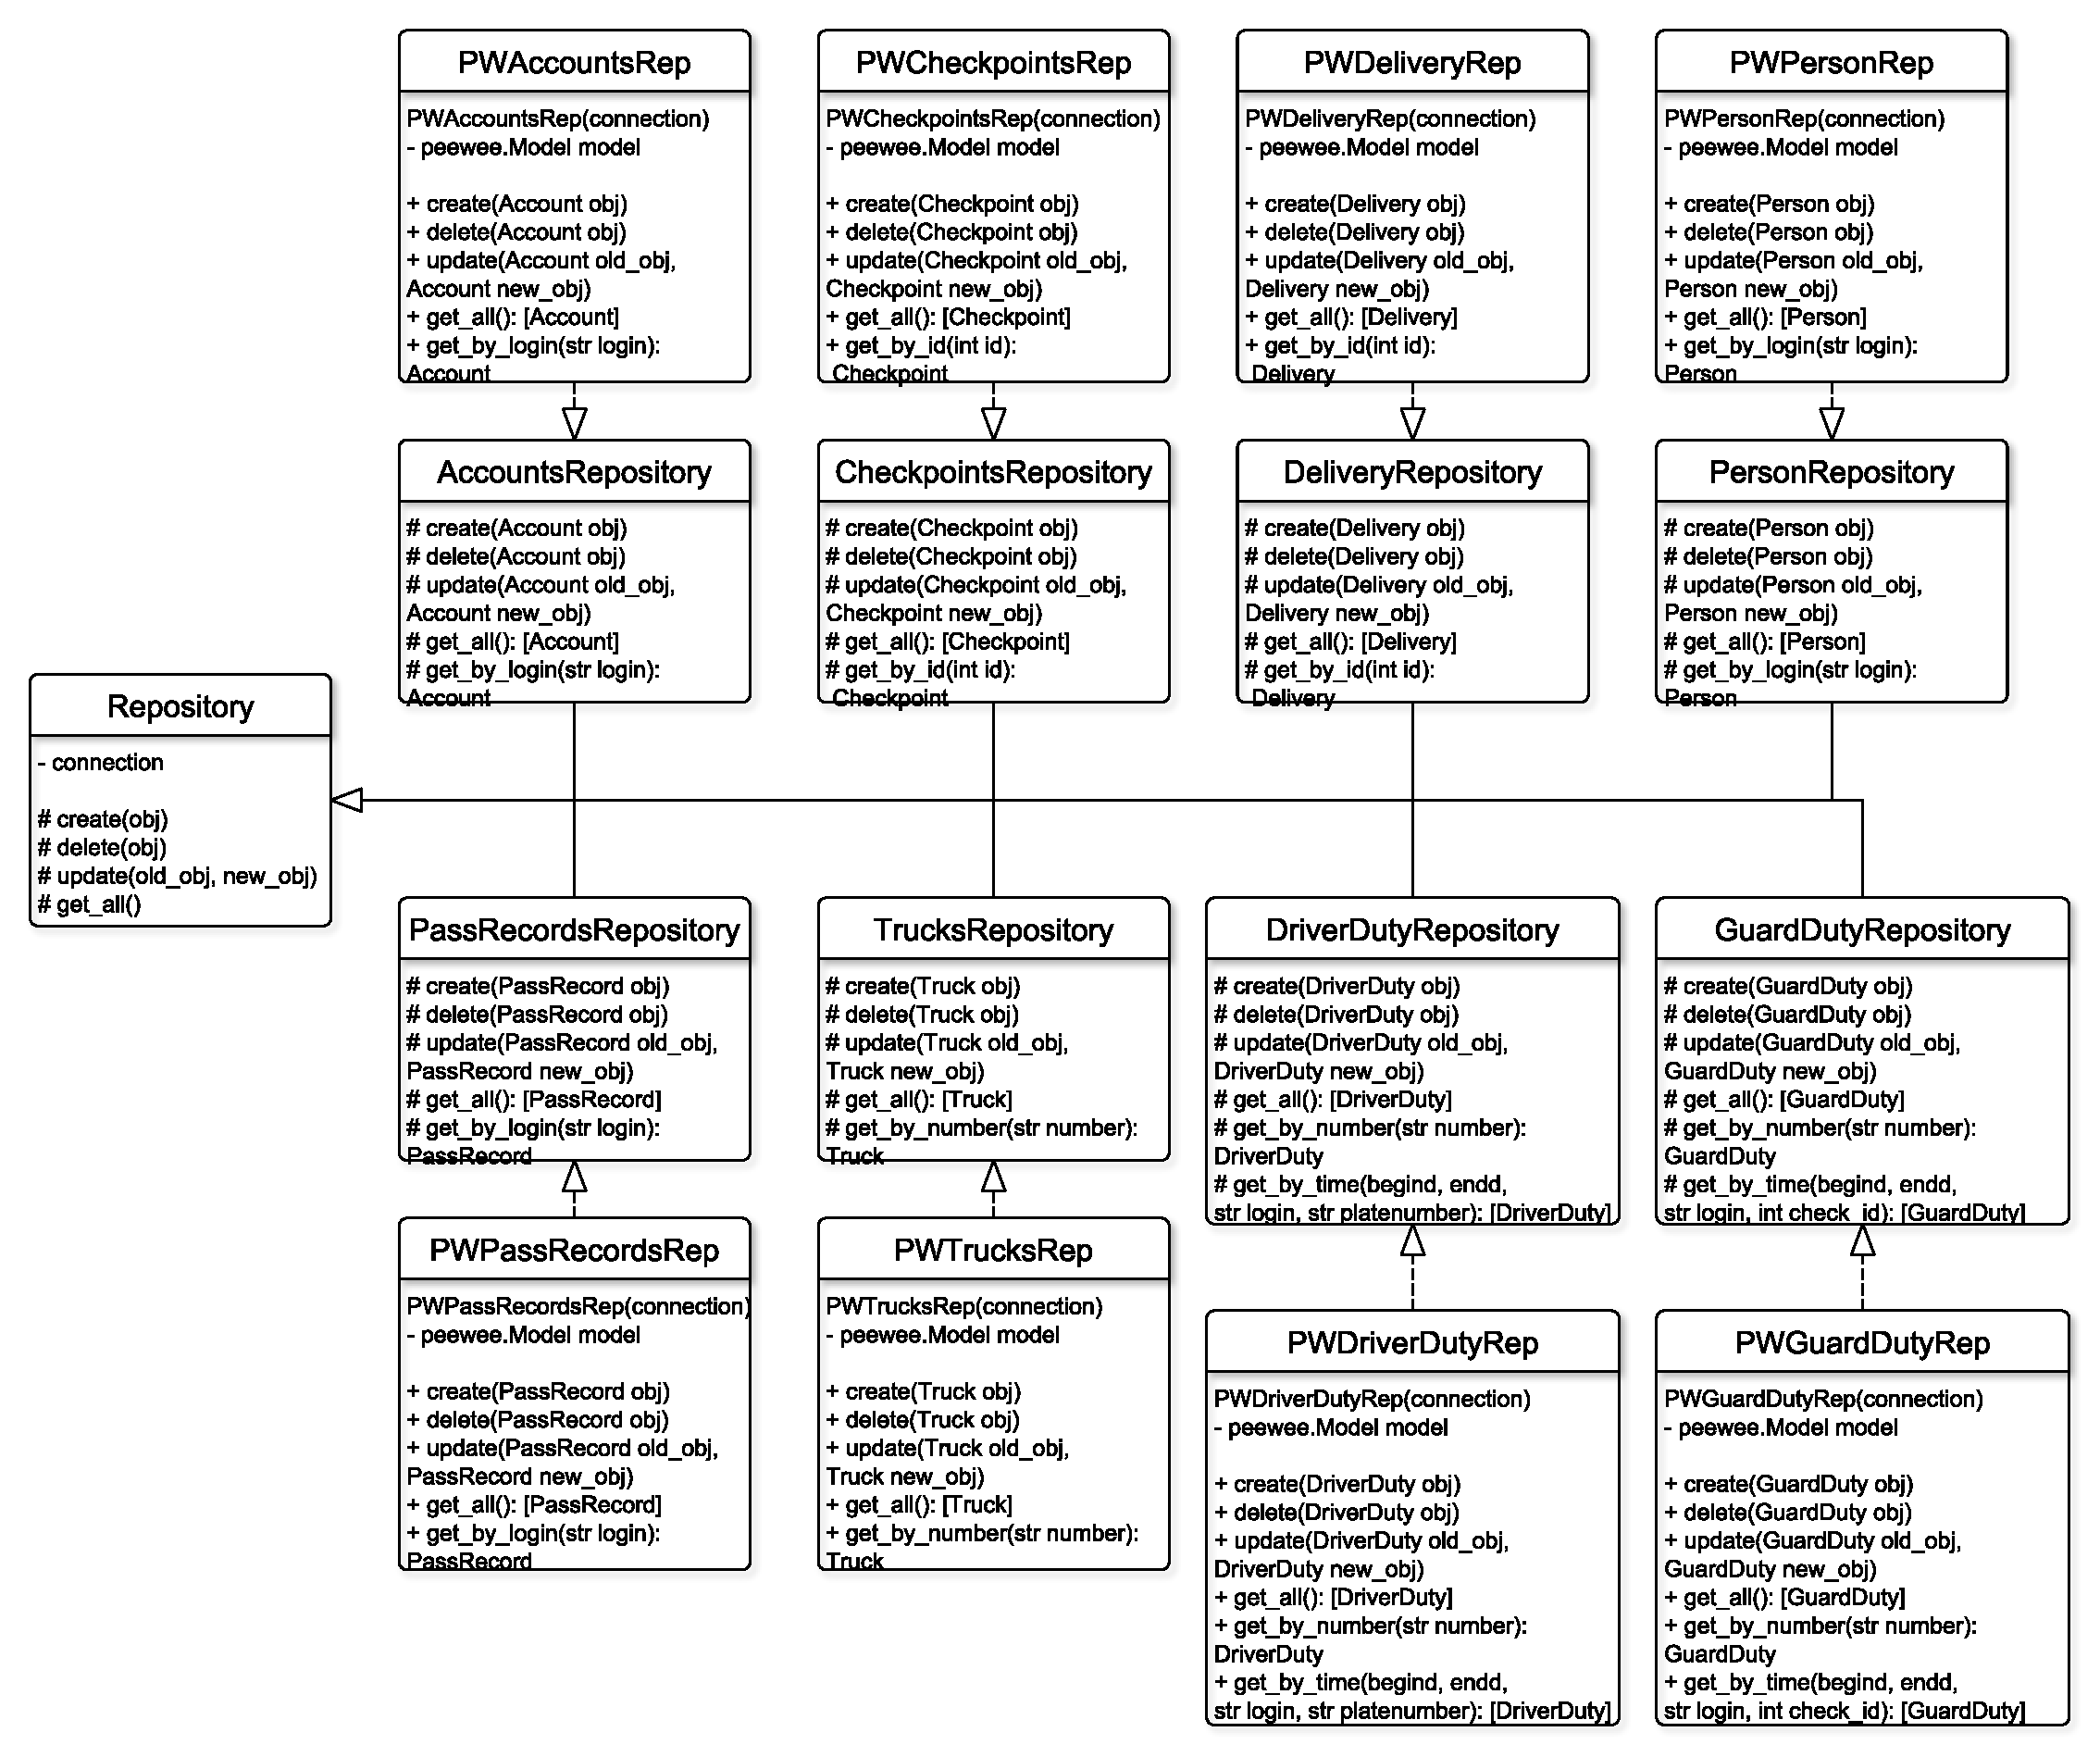
\includegraphics[height=14cm, width = 14cm]{uml/repsoitory.pdf}}
		{\includegraphics[scale=0.43, angle=0]{sc/unver}}
		\caption{Страница просмотра заявок регистрации}
	\end{center}
\end{figure}

\begin{figure}[h!] \label{all_delivery_sc}
	\begin{center}
		%		{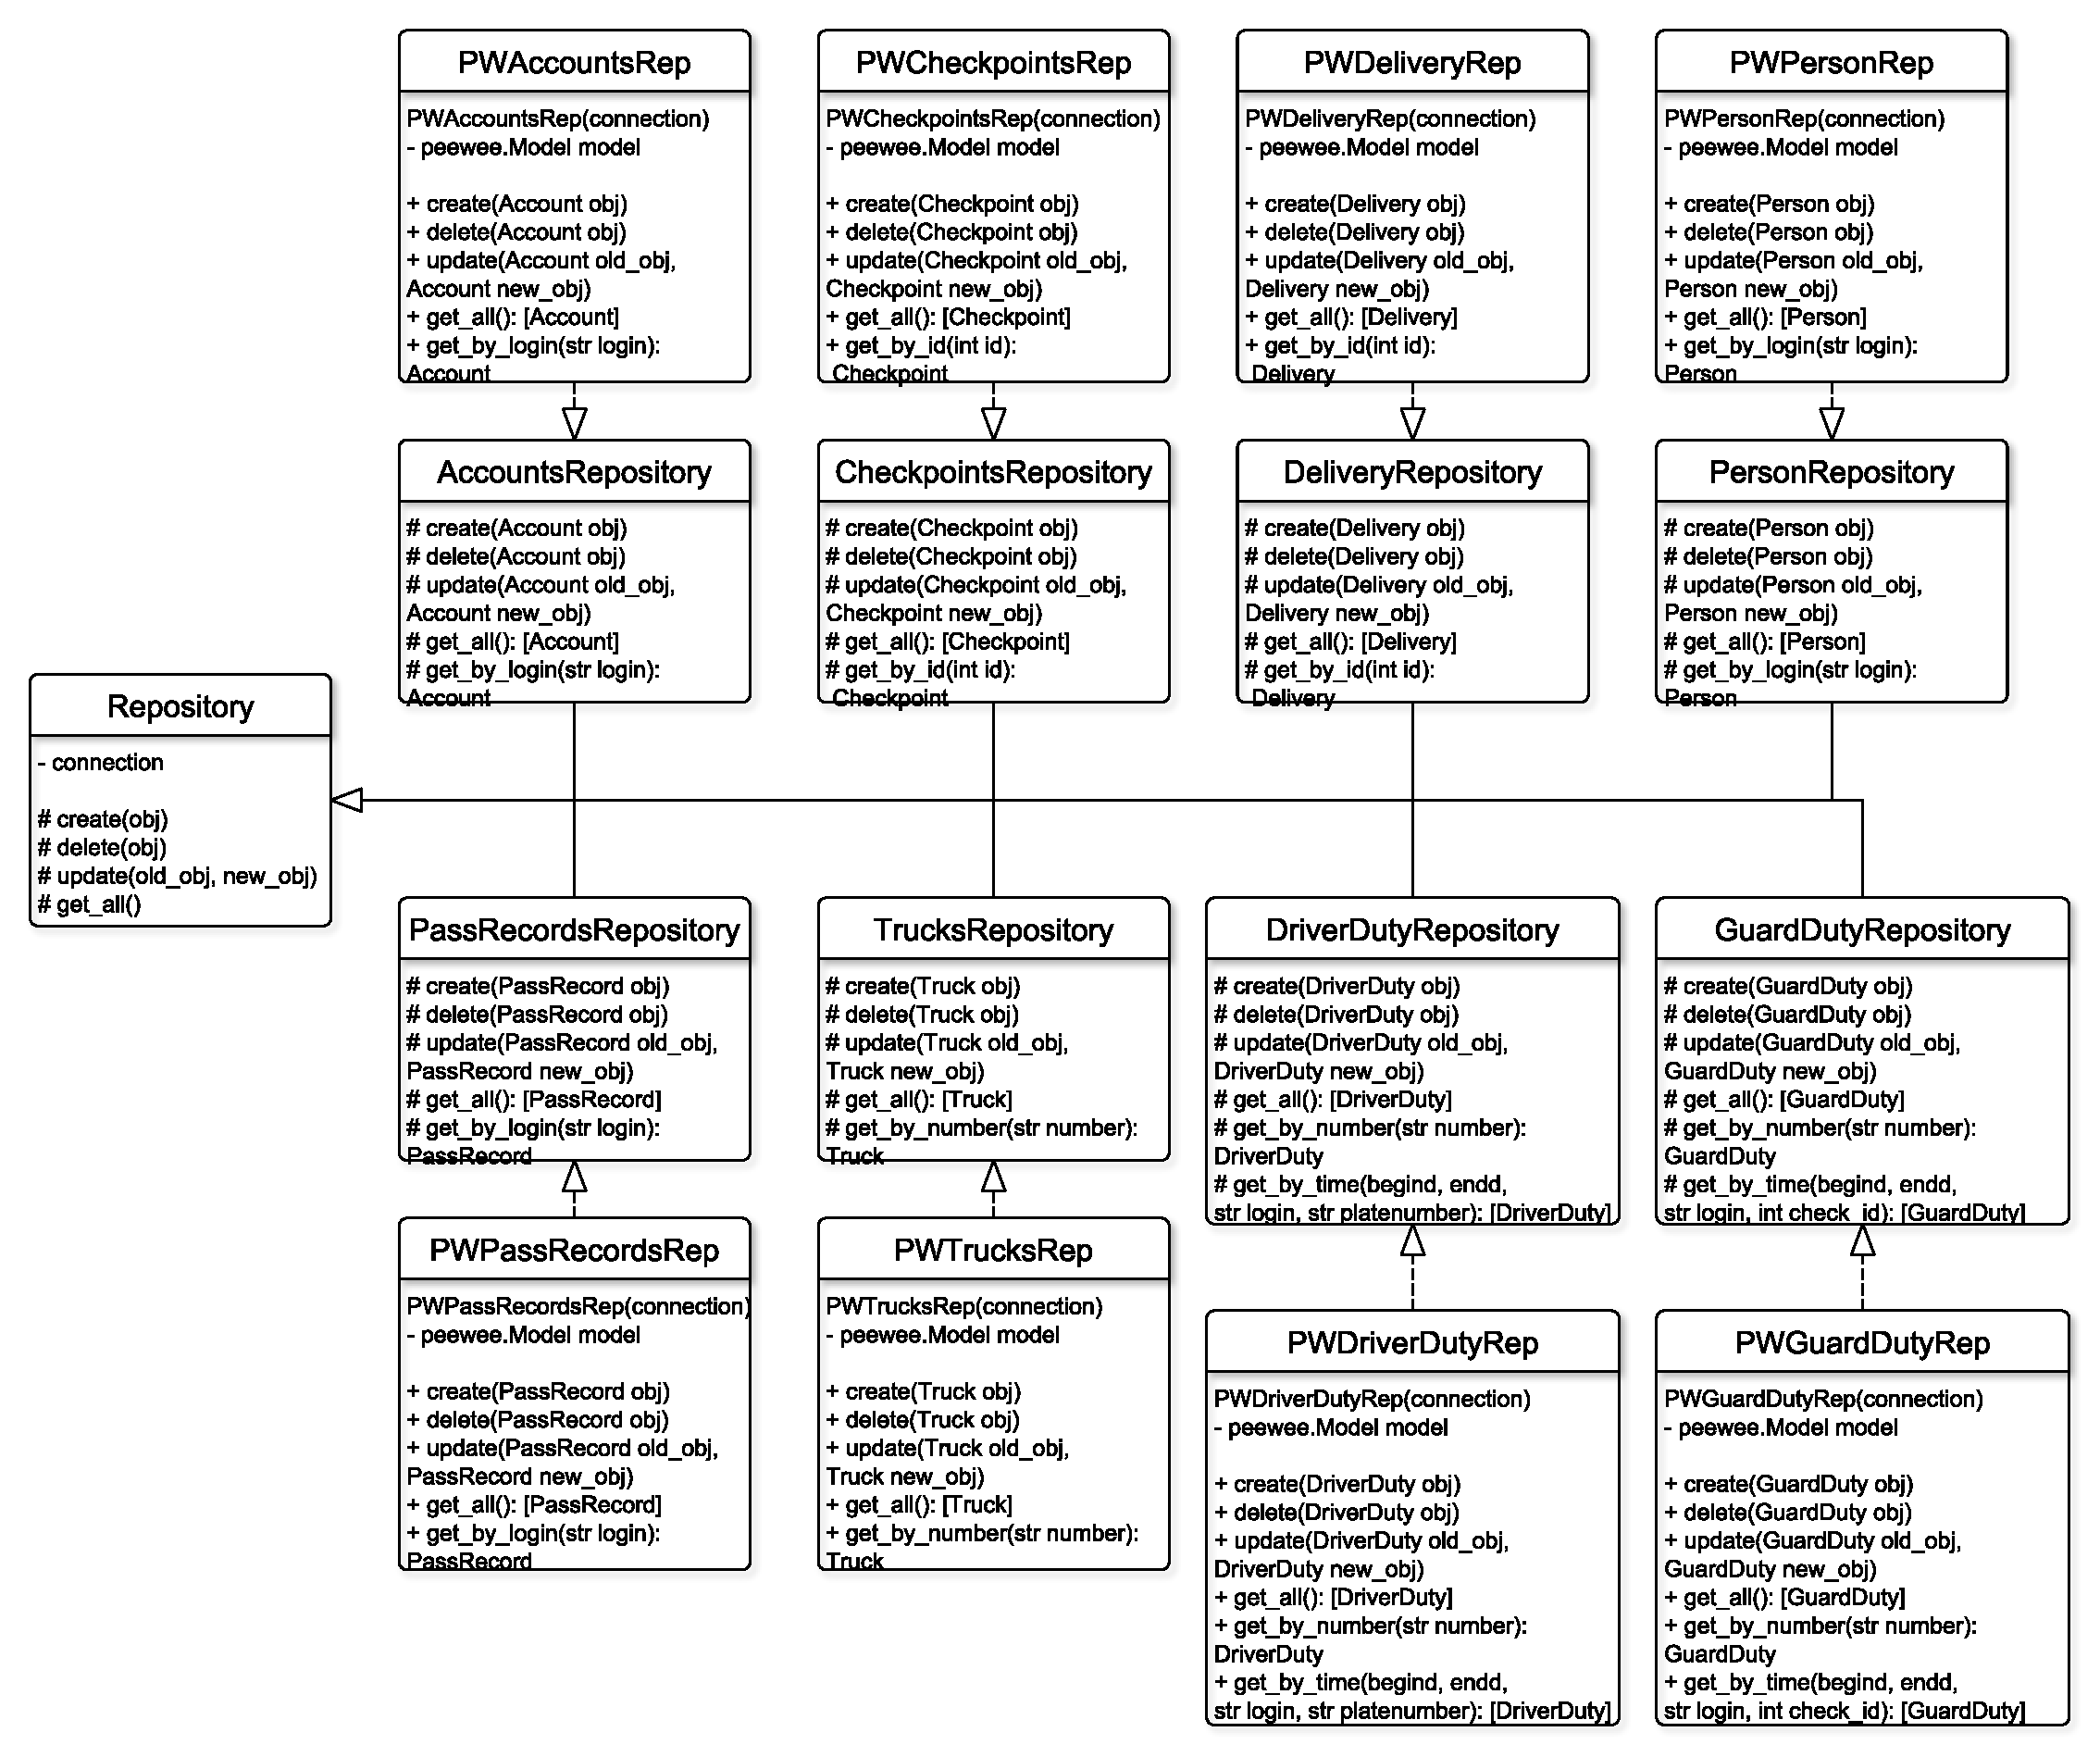
\includegraphics[height=14cm, width = 14cm]{uml/repsoitory.pdf}}
		{\includegraphics[scale=0.43, angle=0]{sc/all_delivery}}
		\caption{Страница просмотра и создания заказов}
	\end{center}
\end{figure}

\begin{figure}[h!] \label{all_pass_sc}
	\begin{center}
		%		{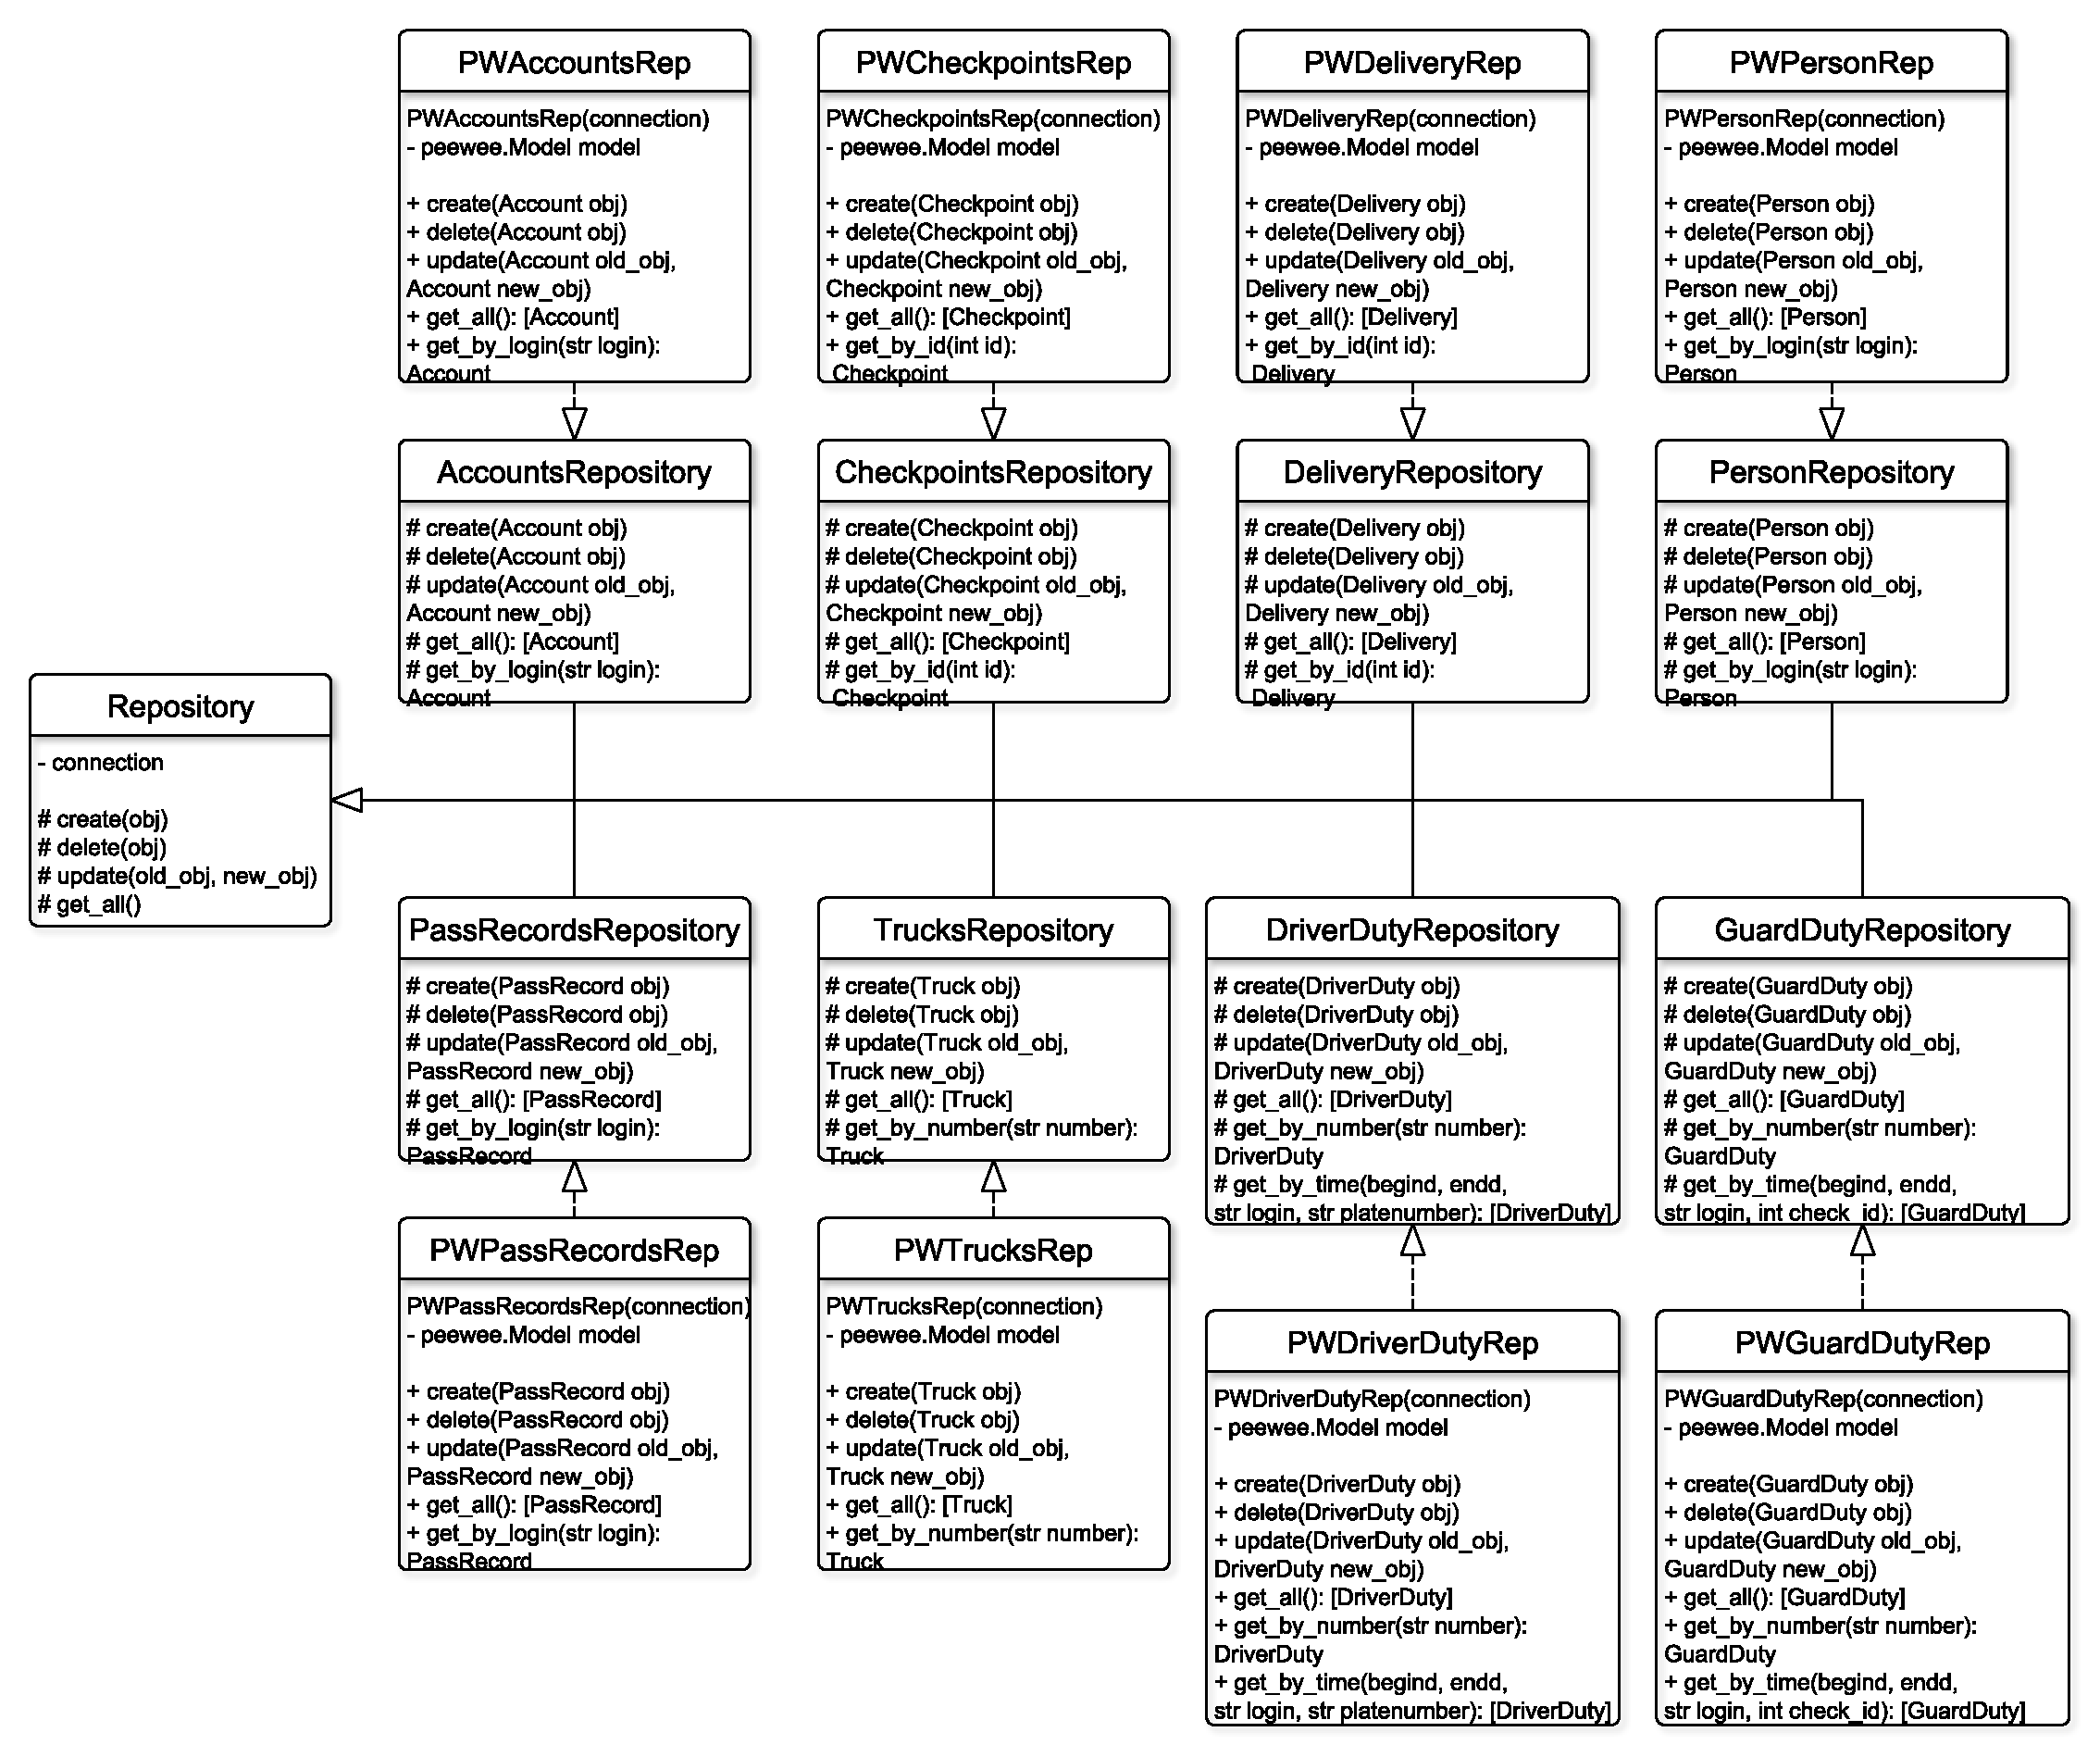
\includegraphics[height=14cm, width = 14cm]{uml/repsoitory.pdf}}
		{\includegraphics[scale=0.43, angle=0]{sc/all_pass}}
		\caption{Страница просмотра и регистрации записей о проездах}
	\end{center}
\end{figure}

\begin{figure}[h!] \label{driver_duty_sc}
	\begin{center}
		%		{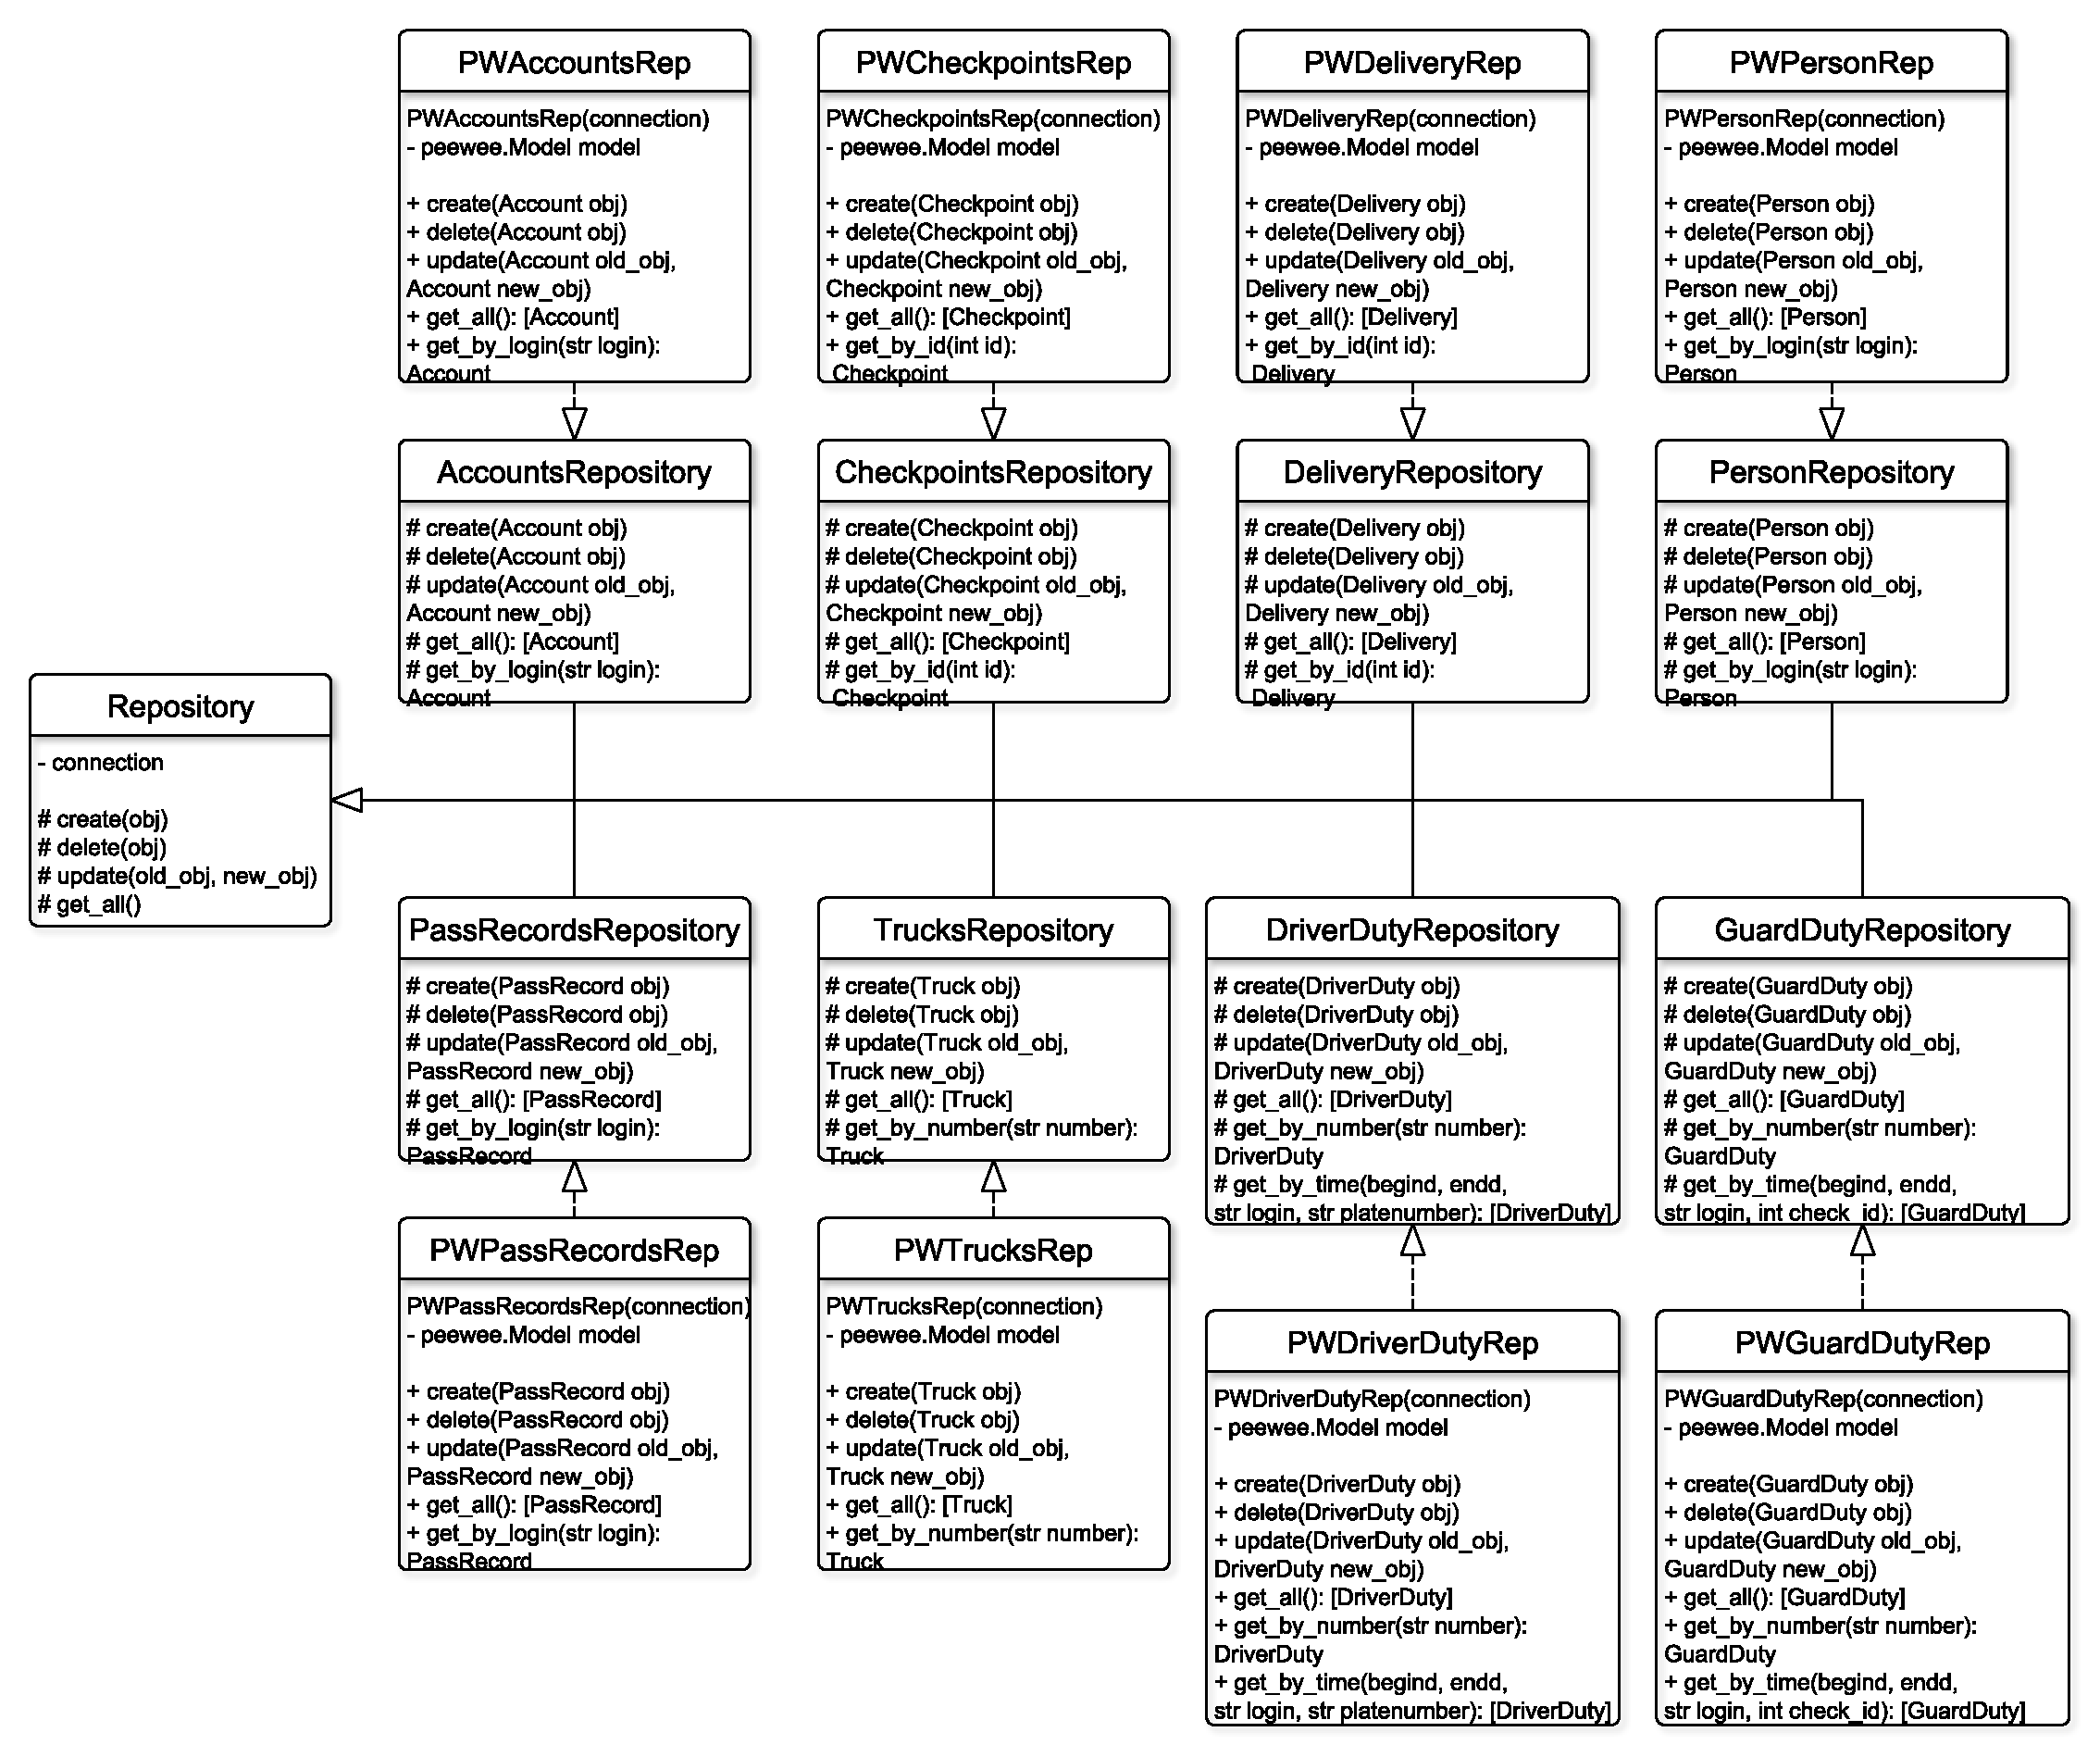
\includegraphics[height=14cm, width = 14cm]{uml/repsoitory.pdf}}
		{\includegraphics[scale=0.43, angle=0]{sc/driver_duty}}
		\caption{Страница просмотра и назначения дежурств водителей}
	\end{center}
\end{figure}

\begin{figure}[h!] \label{trucks_sc}
	\begin{center}
		%		{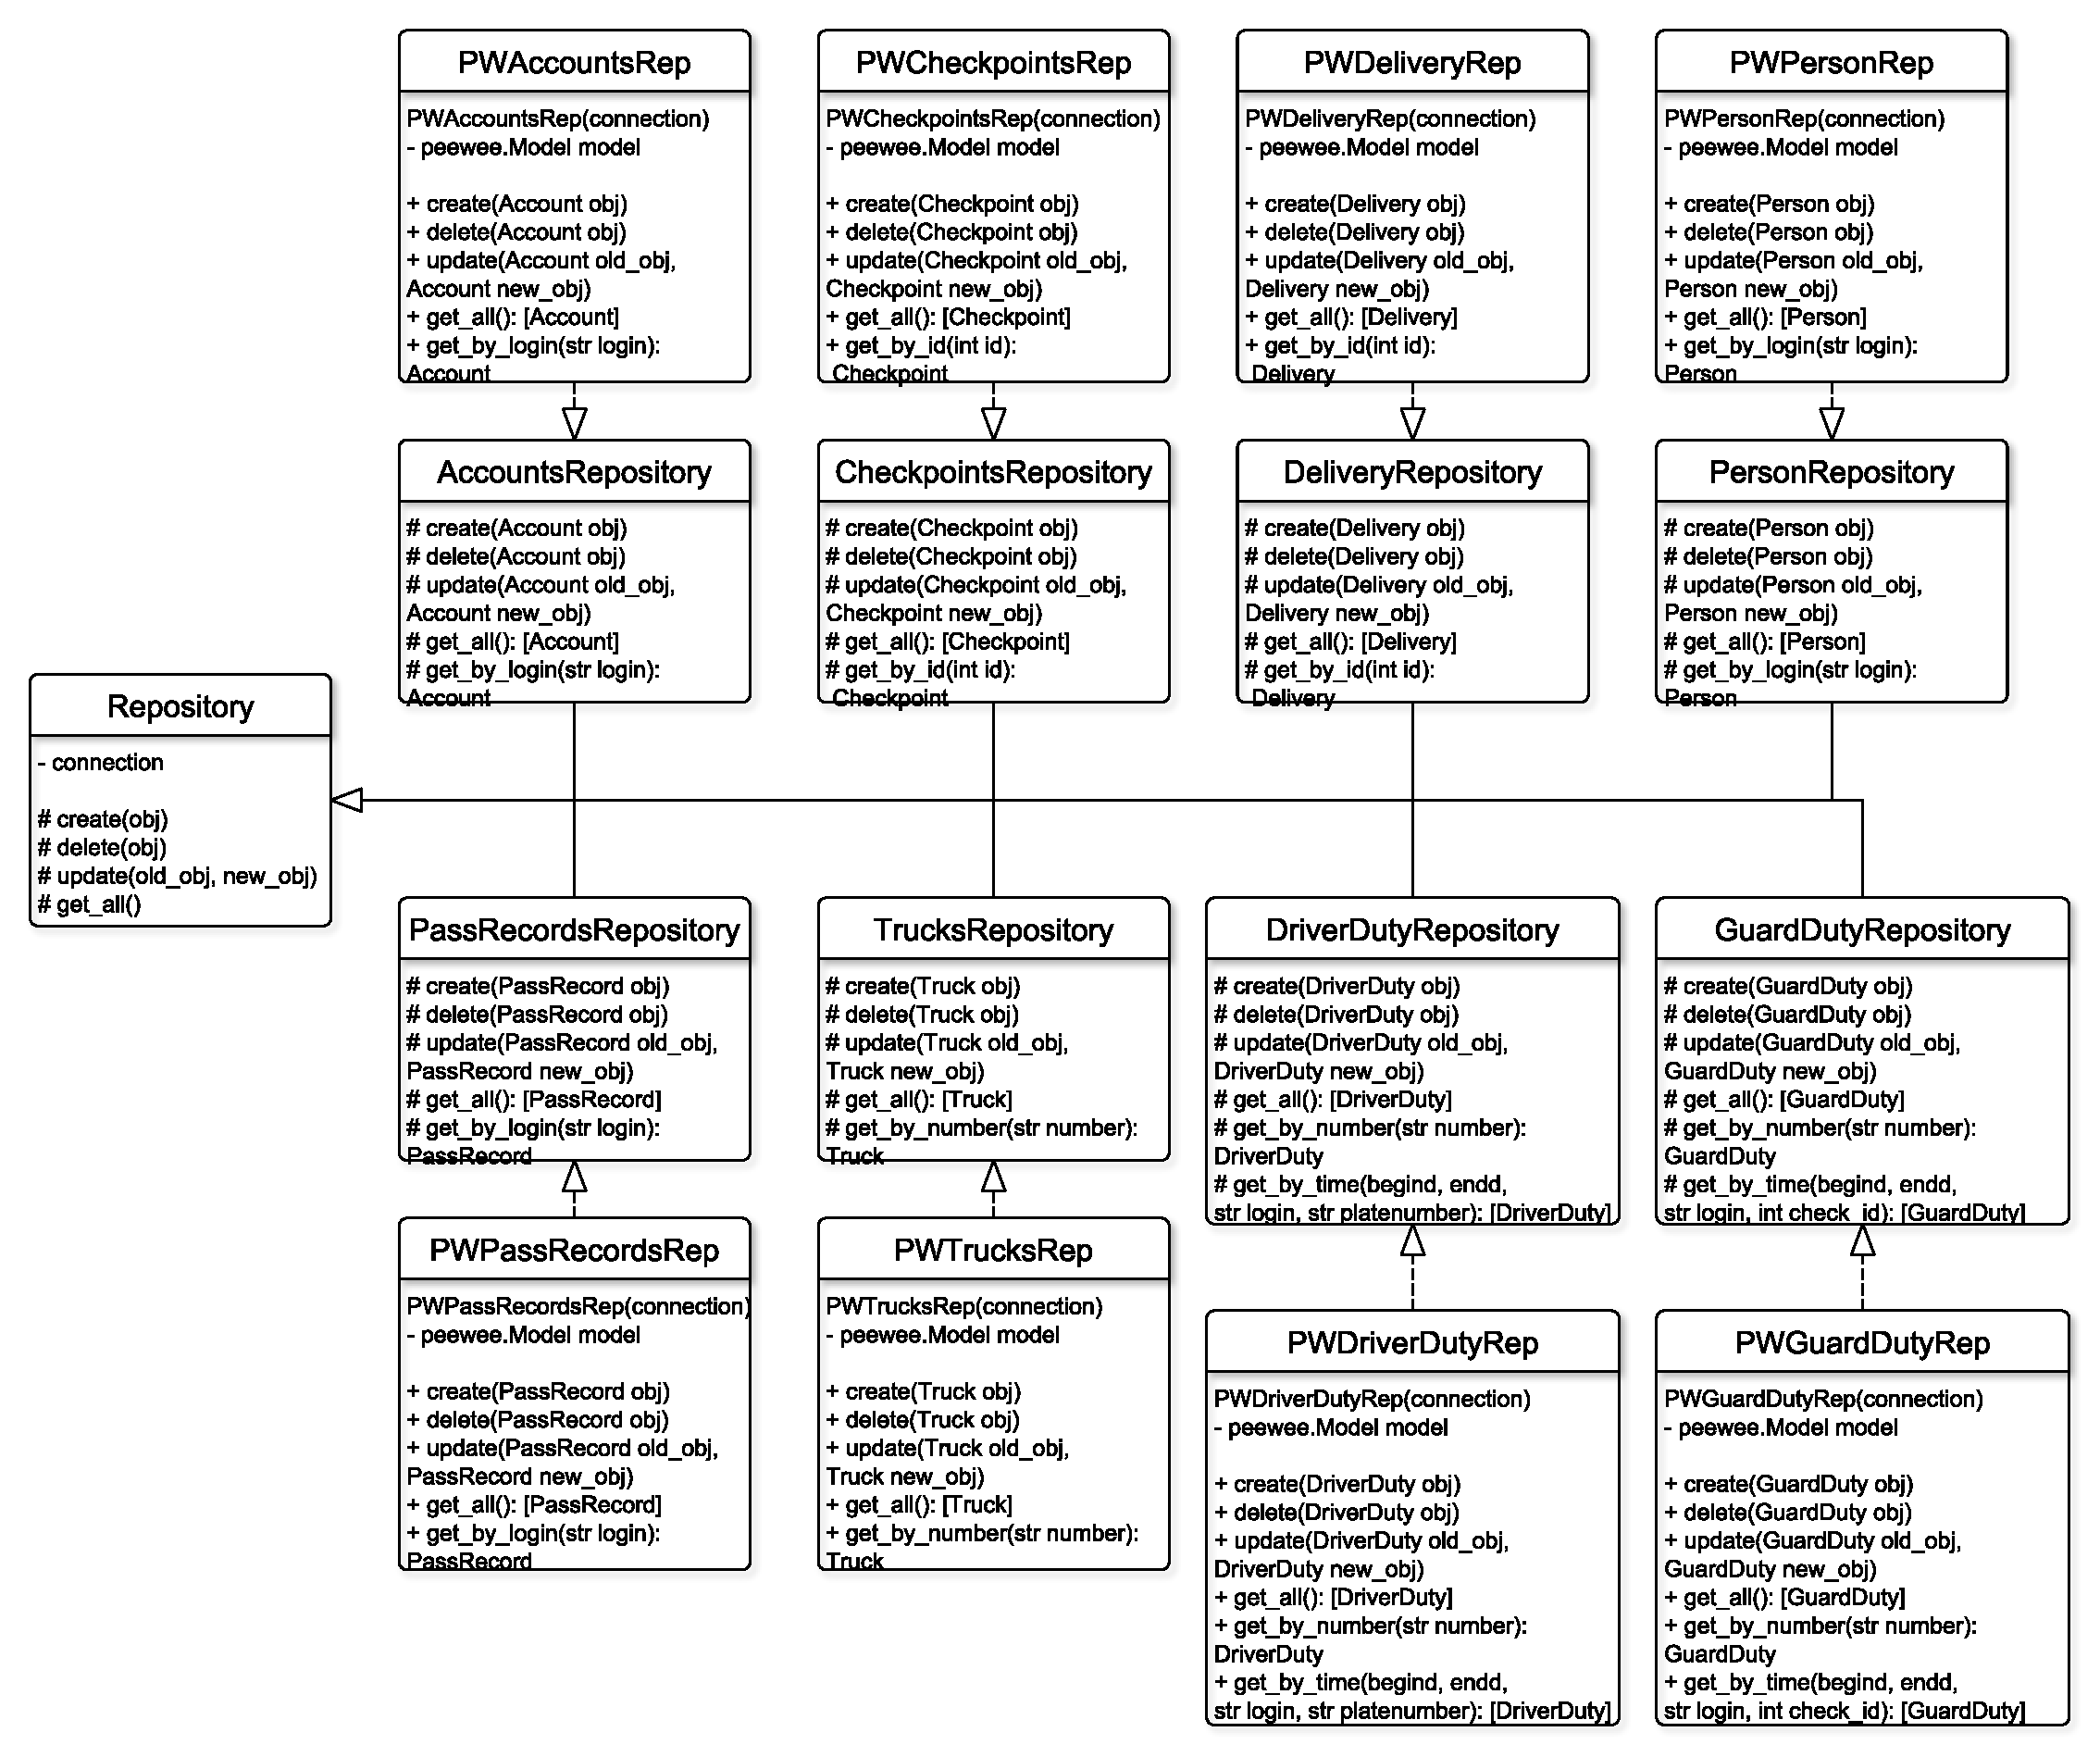
\includegraphics[height=14cm, width = 14cm]{uml/repsoitory.pdf}}
		{\includegraphics[scale=0.43, angle=0]{sc/trucks}}
		\caption{Страница просмотра и регистрации машин}
	\end{center}
\end{figure}

\begin{figure}[h!] \label{pick_delivery_sc}
	\begin{center}
		%		{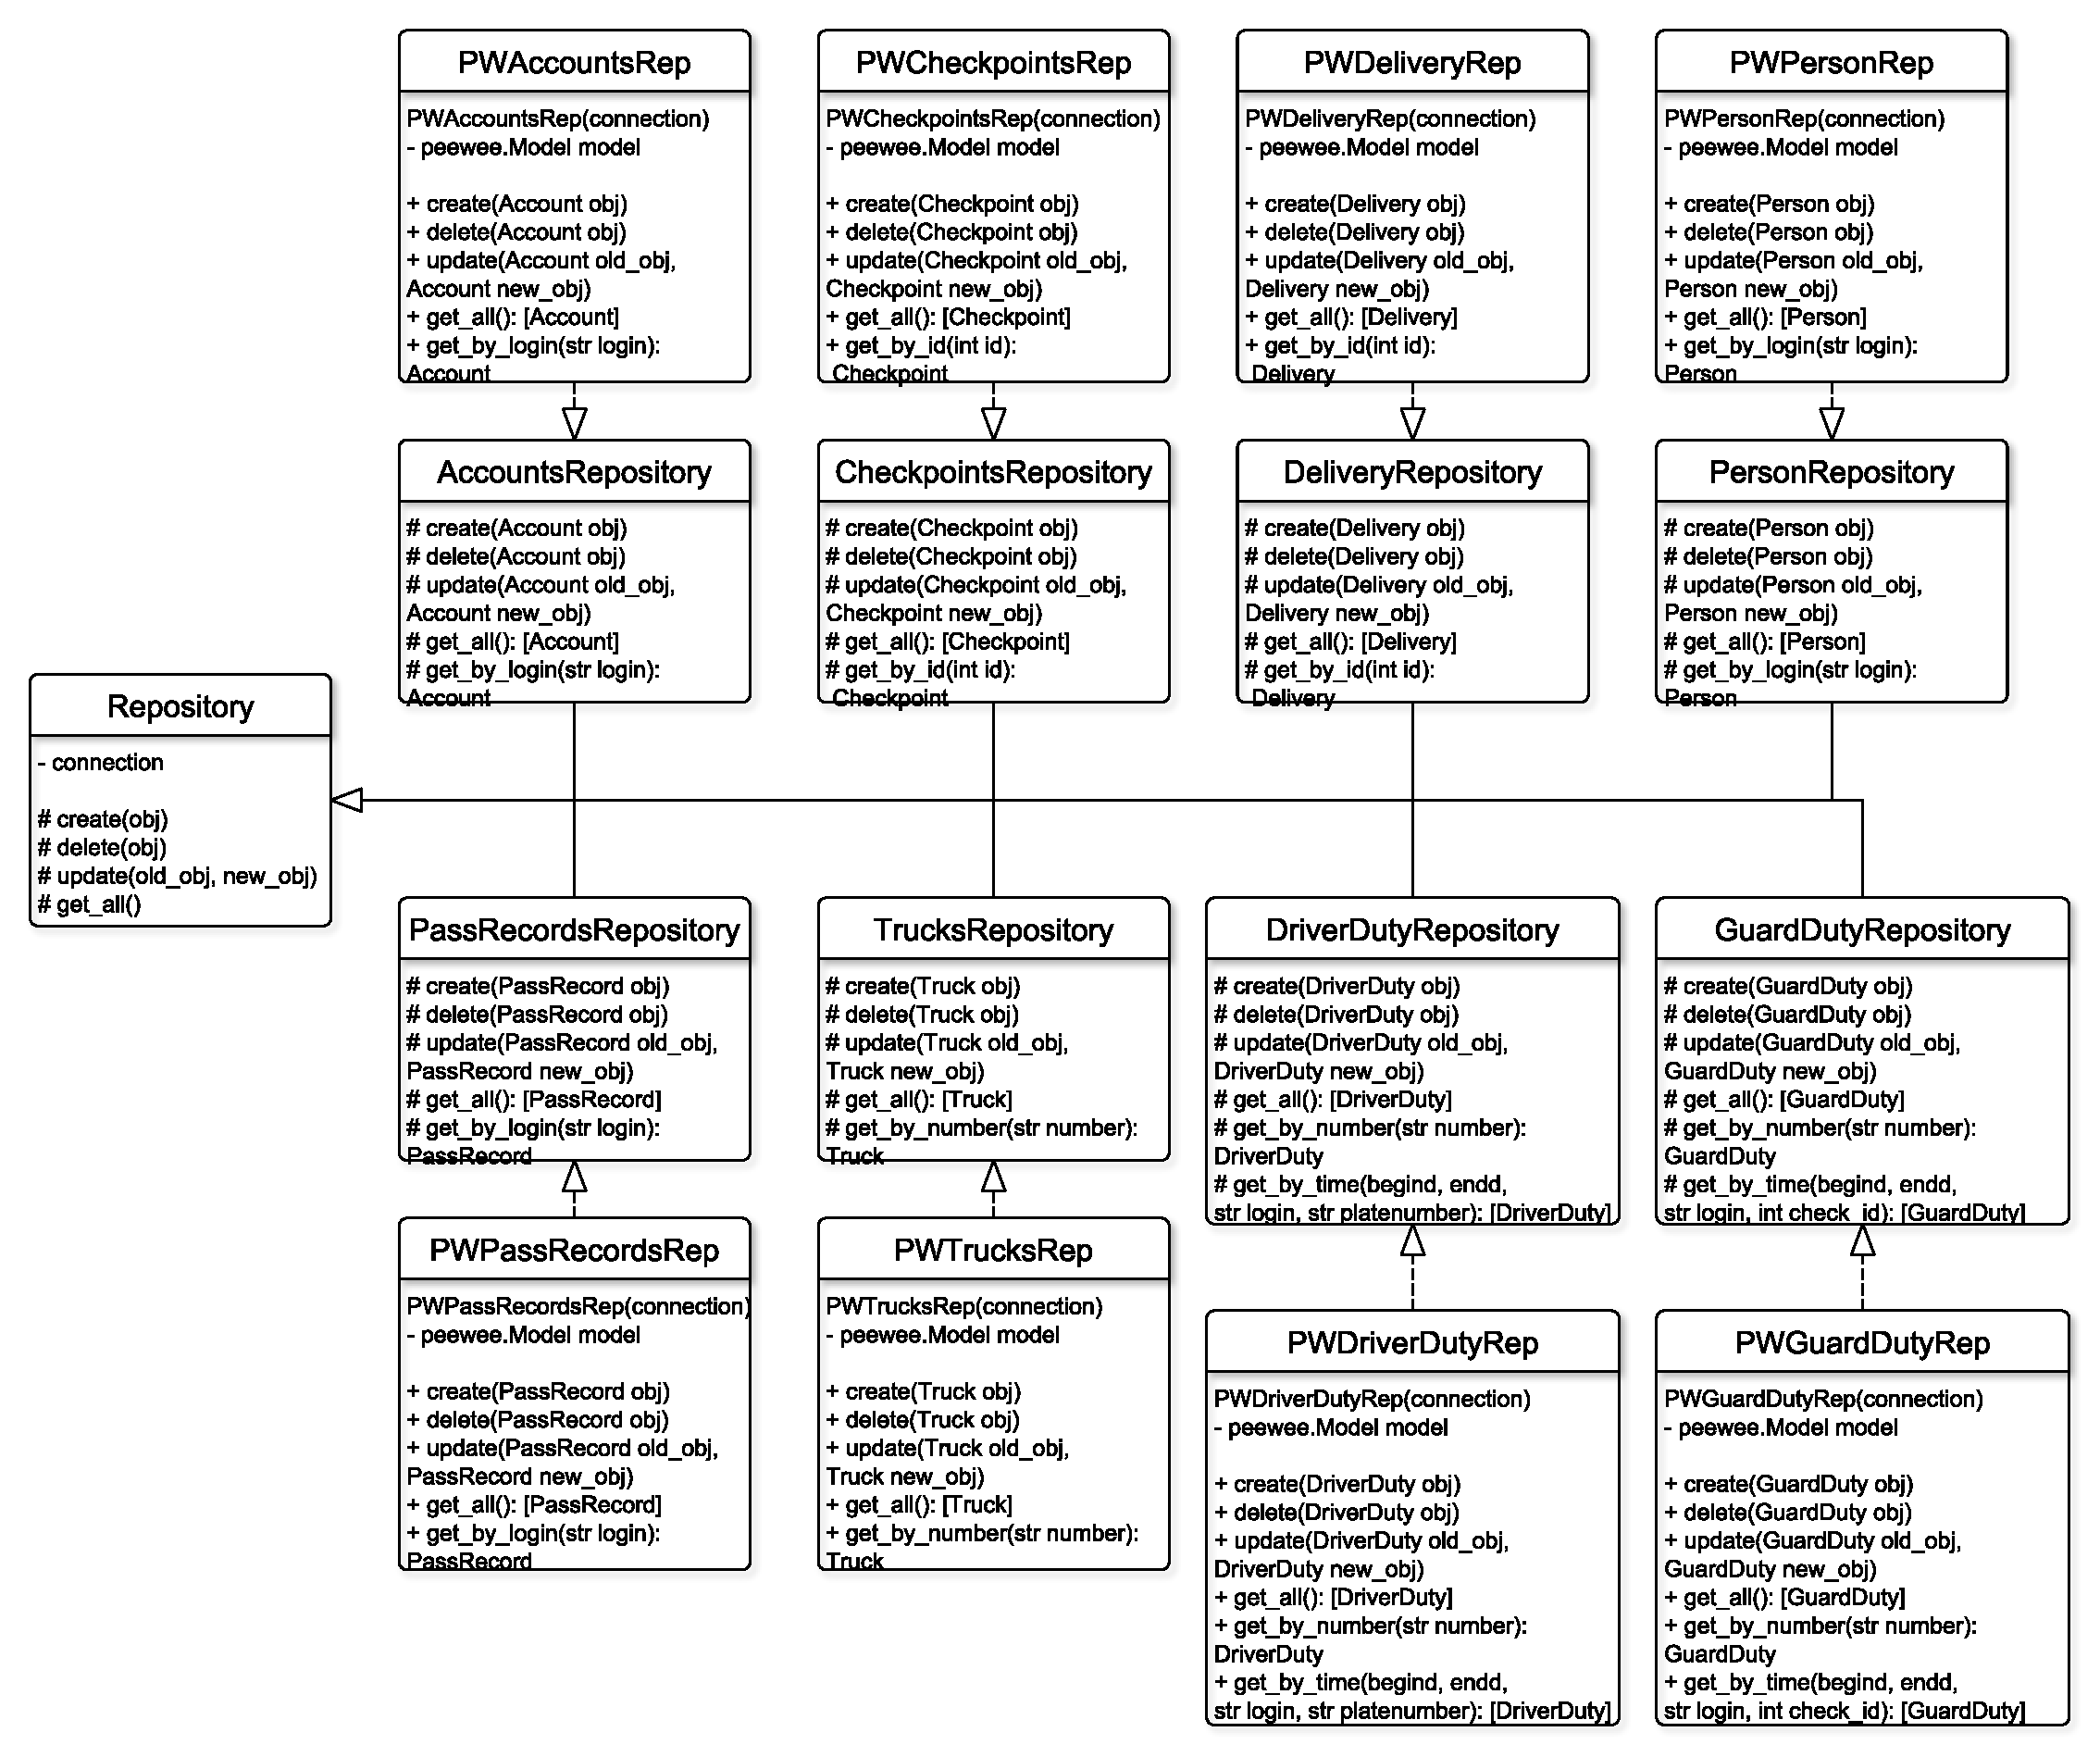
\includegraphics[height=14cm, width = 14cm]{uml/repsoitory.pdf}}
		{\includegraphics[scale=0.4, angle=0]{sc/pick_delivery}}
		\caption{Страница просмотра и выбора заказа (для роли водителя)}
	\end{center}
\end{figure}

\begin{figure}[h!] \label{driver_profile_sc}
	\begin{center}
		%		{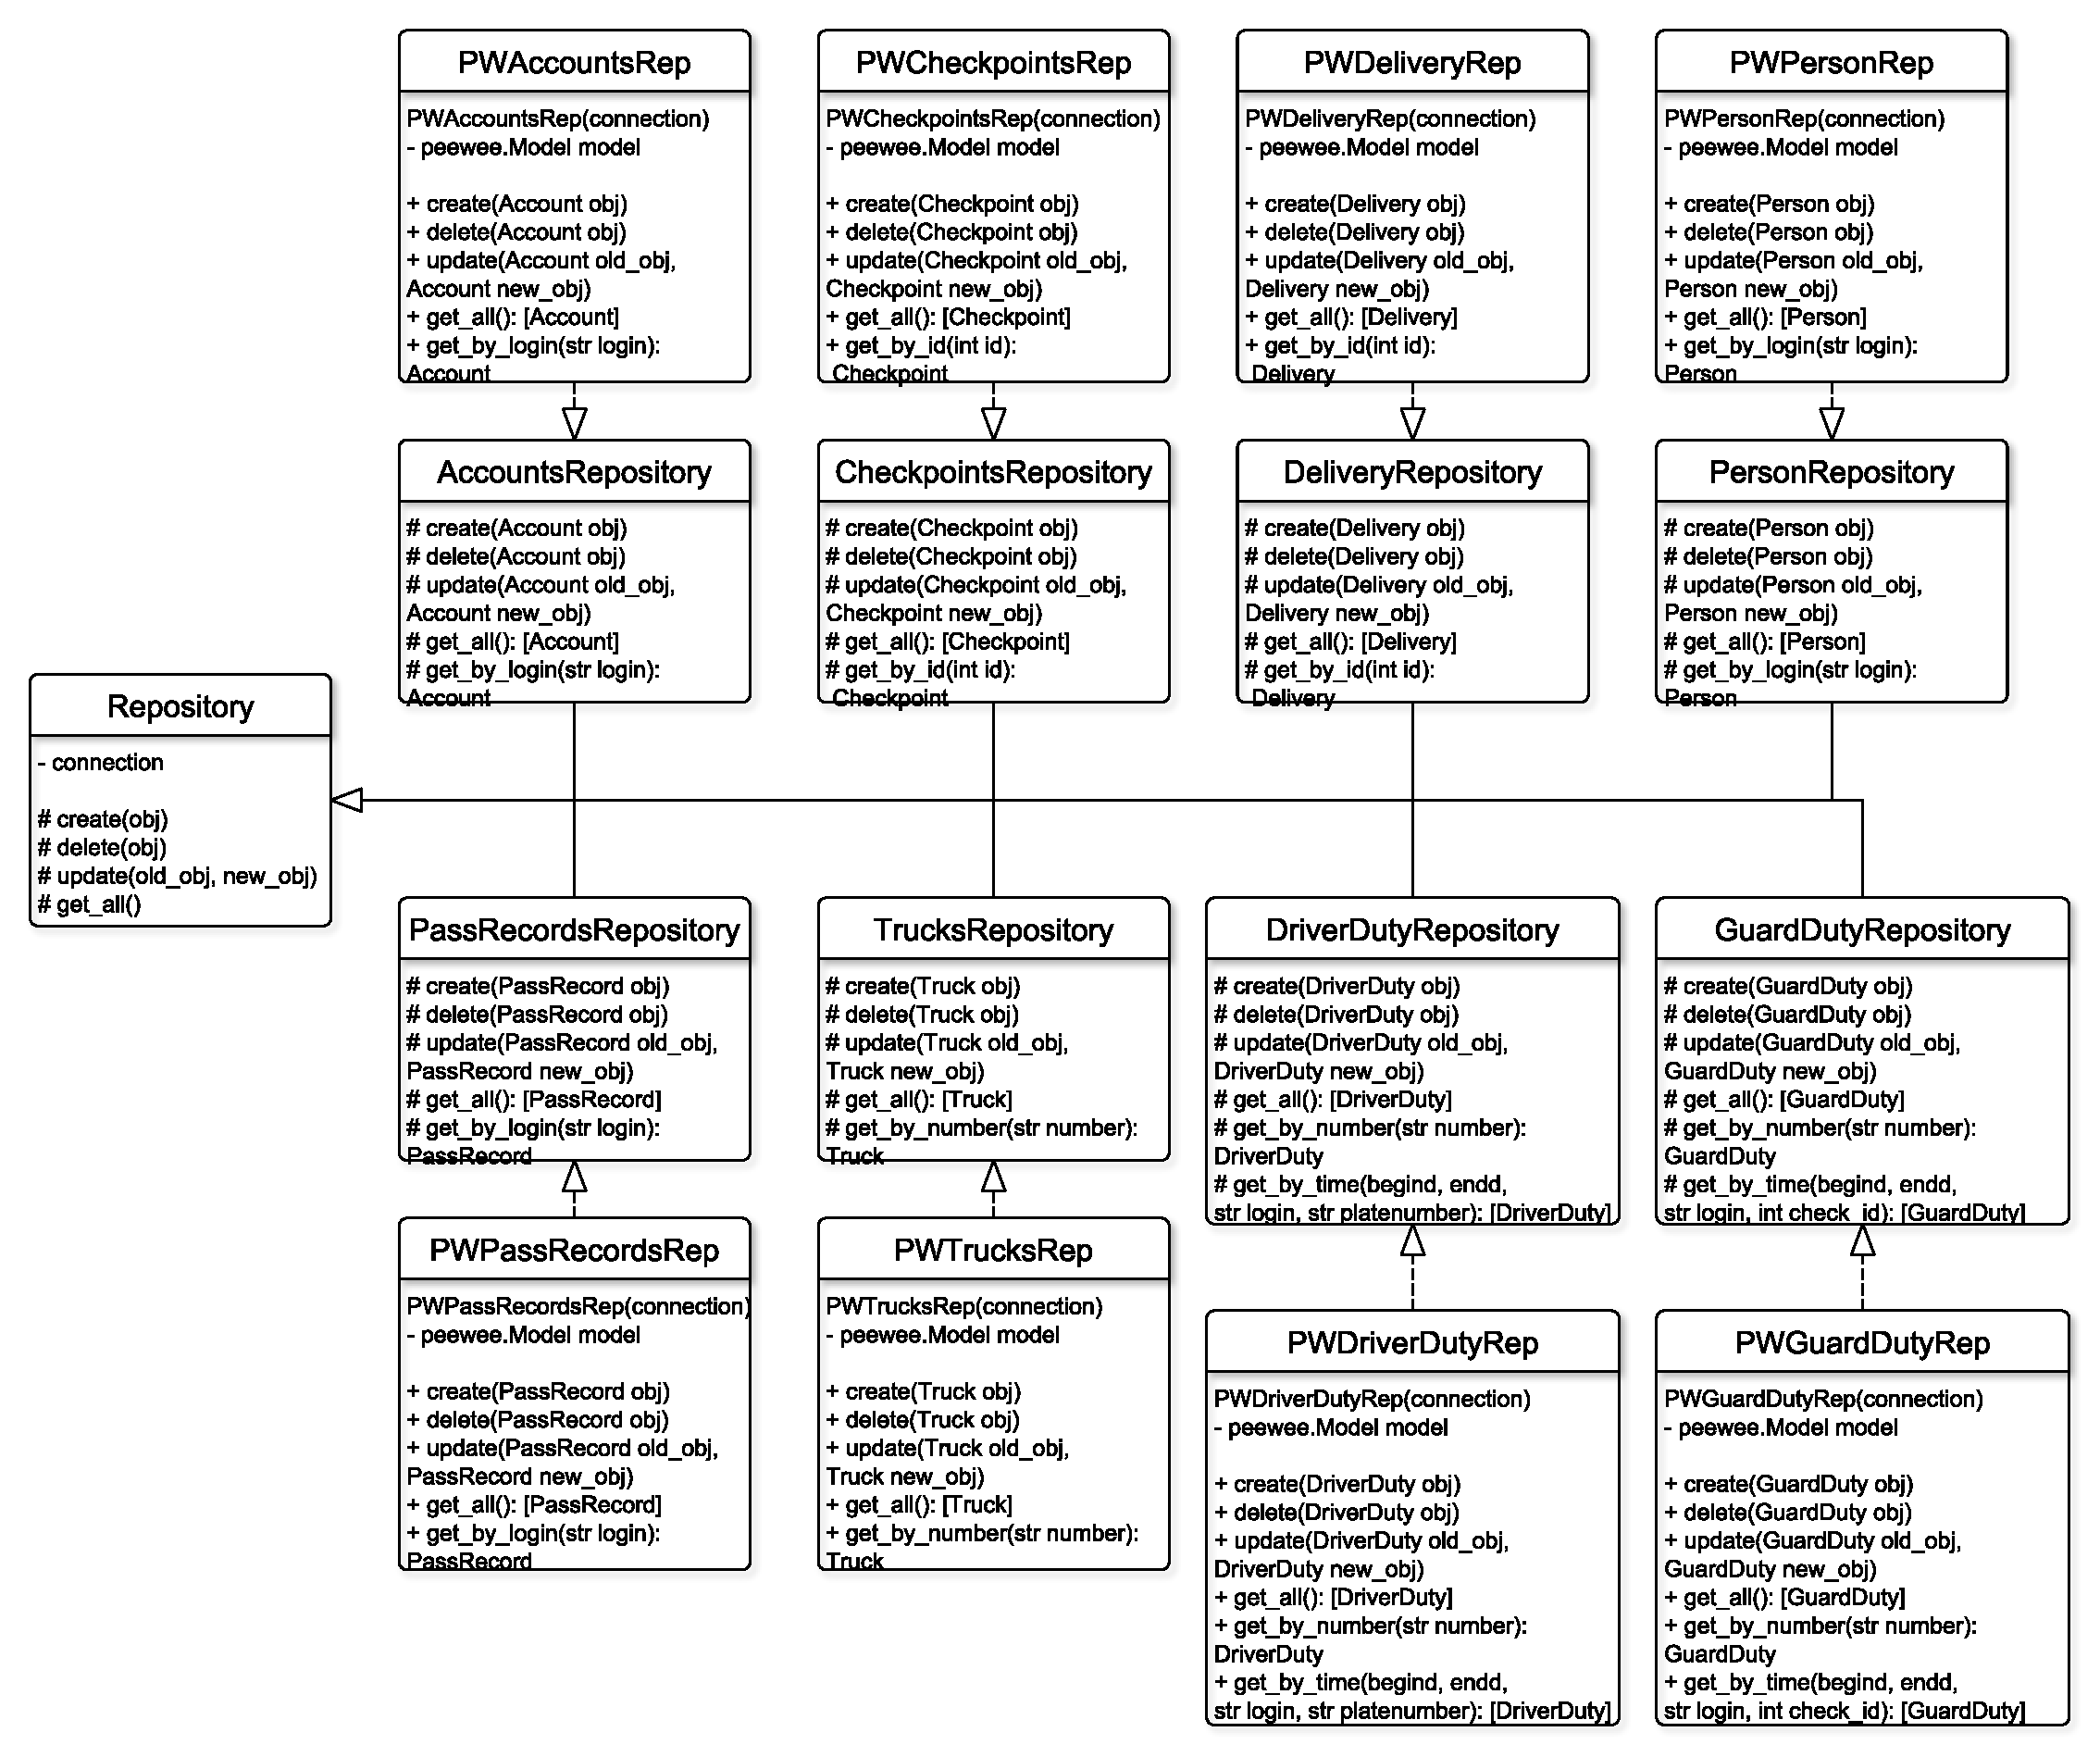
\includegraphics[height=14cm, width = 14cm]{uml/repsoitory.pdf}}
		{\includegraphics[scale=0.4, angle=0]{sc/driver_profile}}
		\caption{Личная страница (для роли водителя)}
	\end{center}
\end{figure}

\begin{figure}[h!] \label{guard_duty_sc}
	\begin{center}
		%		{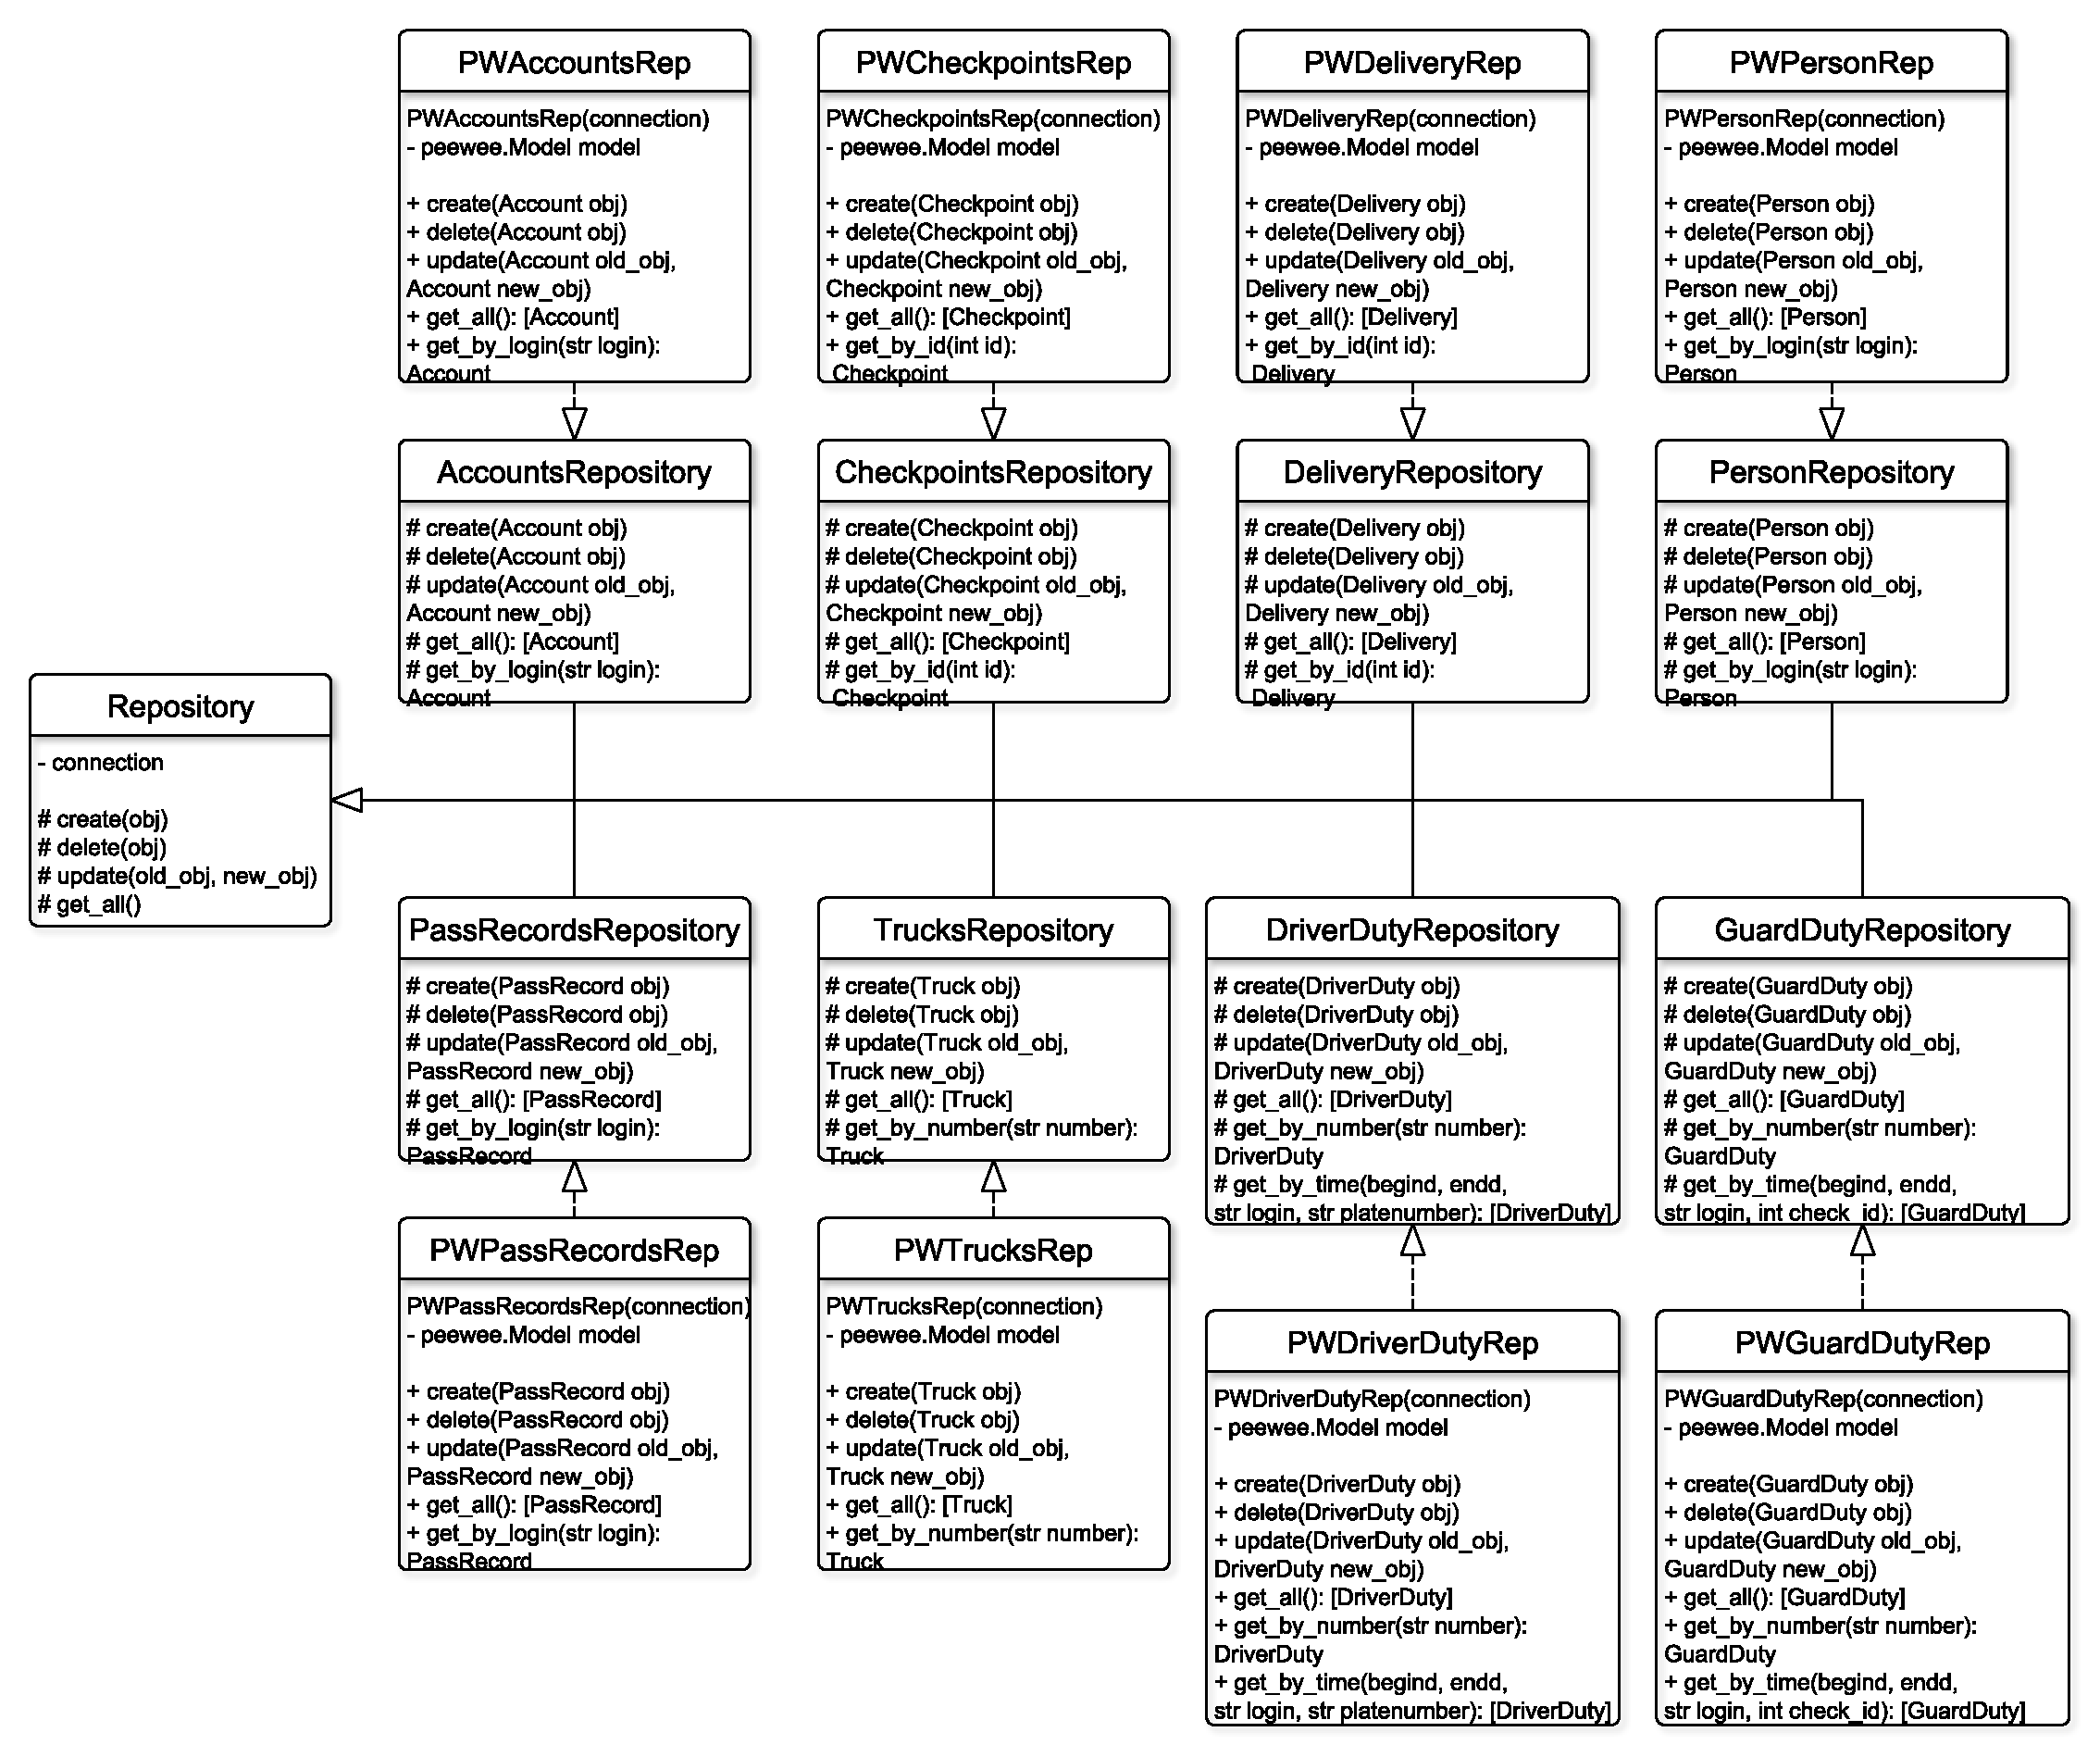
\includegraphics[height=14cm, width = 14cm]{uml/repsoitory.pdf}}
		{\includegraphics[scale=0.4, angle=0]{sc/guard_duty}}
		\caption{Страница просмотра дежурств (для роли охранника)}
	\end{center}
\end{figure}

\begin{figure}[h!] \label{pass_guard_sc}
	\begin{center}
		%		{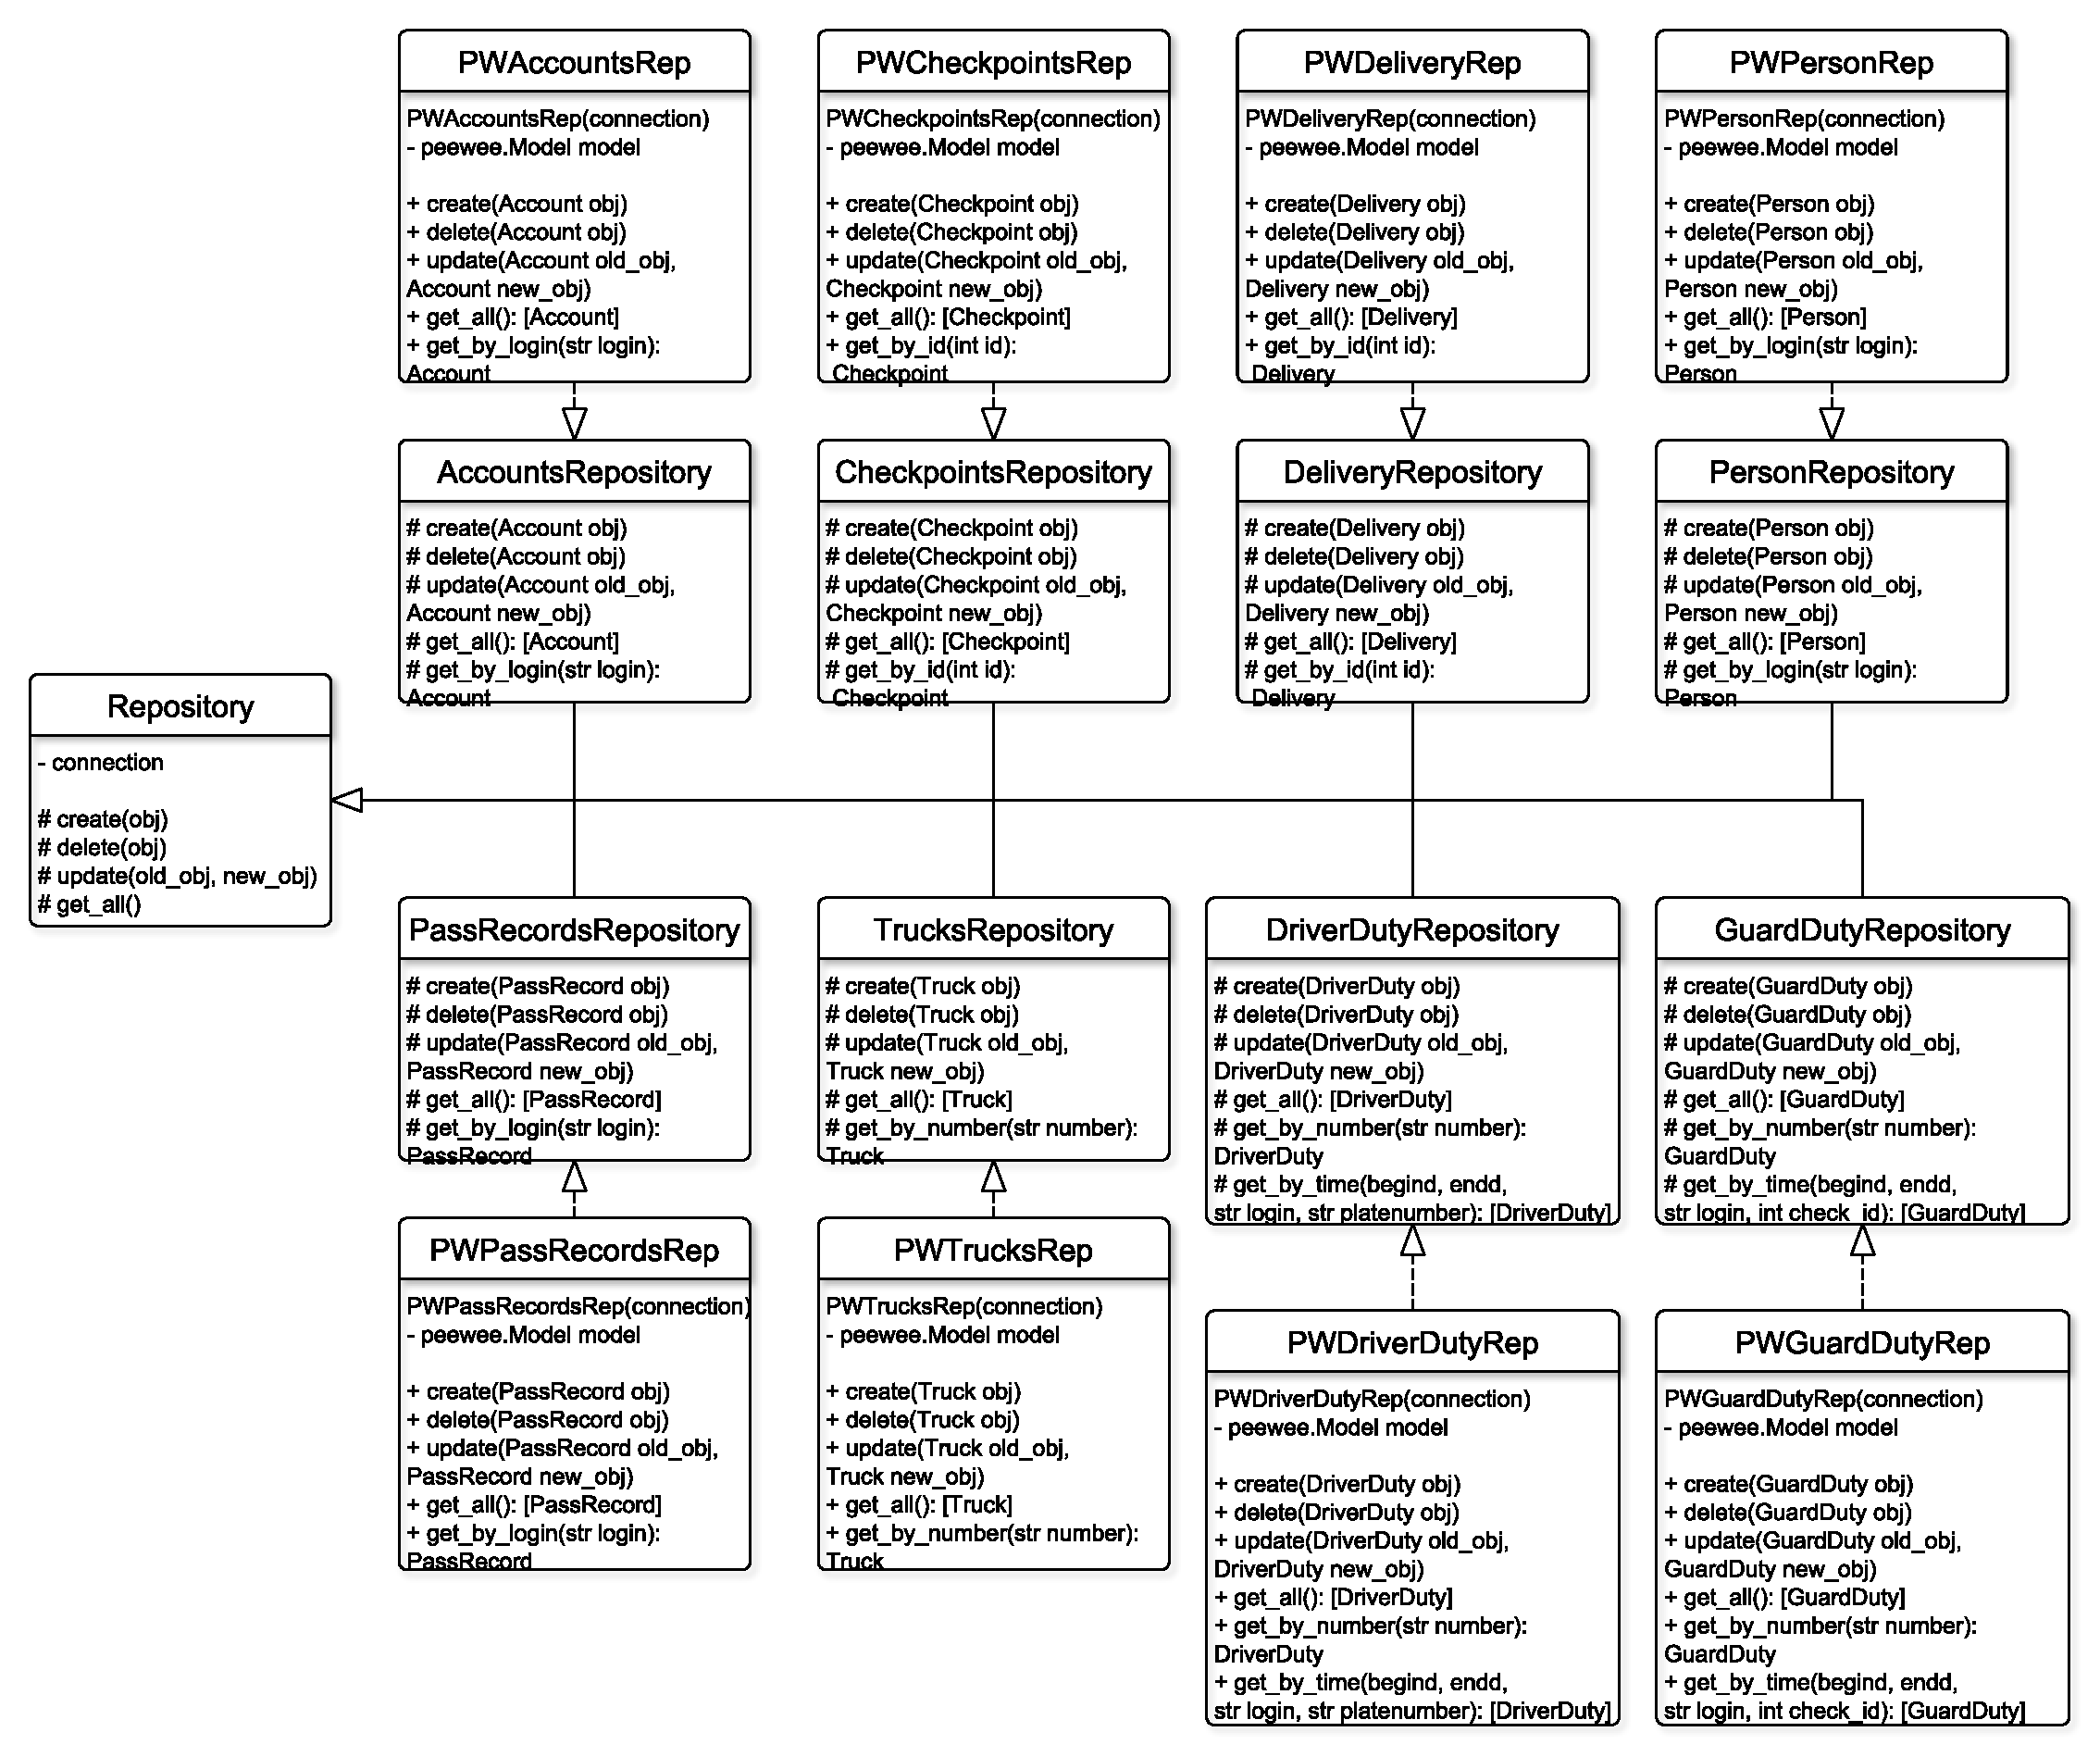
\includegraphics[height=14cm, width = 14cm]{uml/repsoitory.pdf}}
		{\includegraphics[scale=0.4, angle=0]{sc/pass_guard}}
		\caption{Страница просмотра и добавления записей проездов (для роли охранника)}
	\end{center}
\end{figure}

\newpage
Для неавторизованного пользователя доступны страницы входа в аккаунт и регистрации (рисунок \hyperref[login_sc]{3.16} и \hyperref[signup_sc]{3.17}) 

\begin{figure}[h!] \label{login_sc}
	\begin{center}
		%		{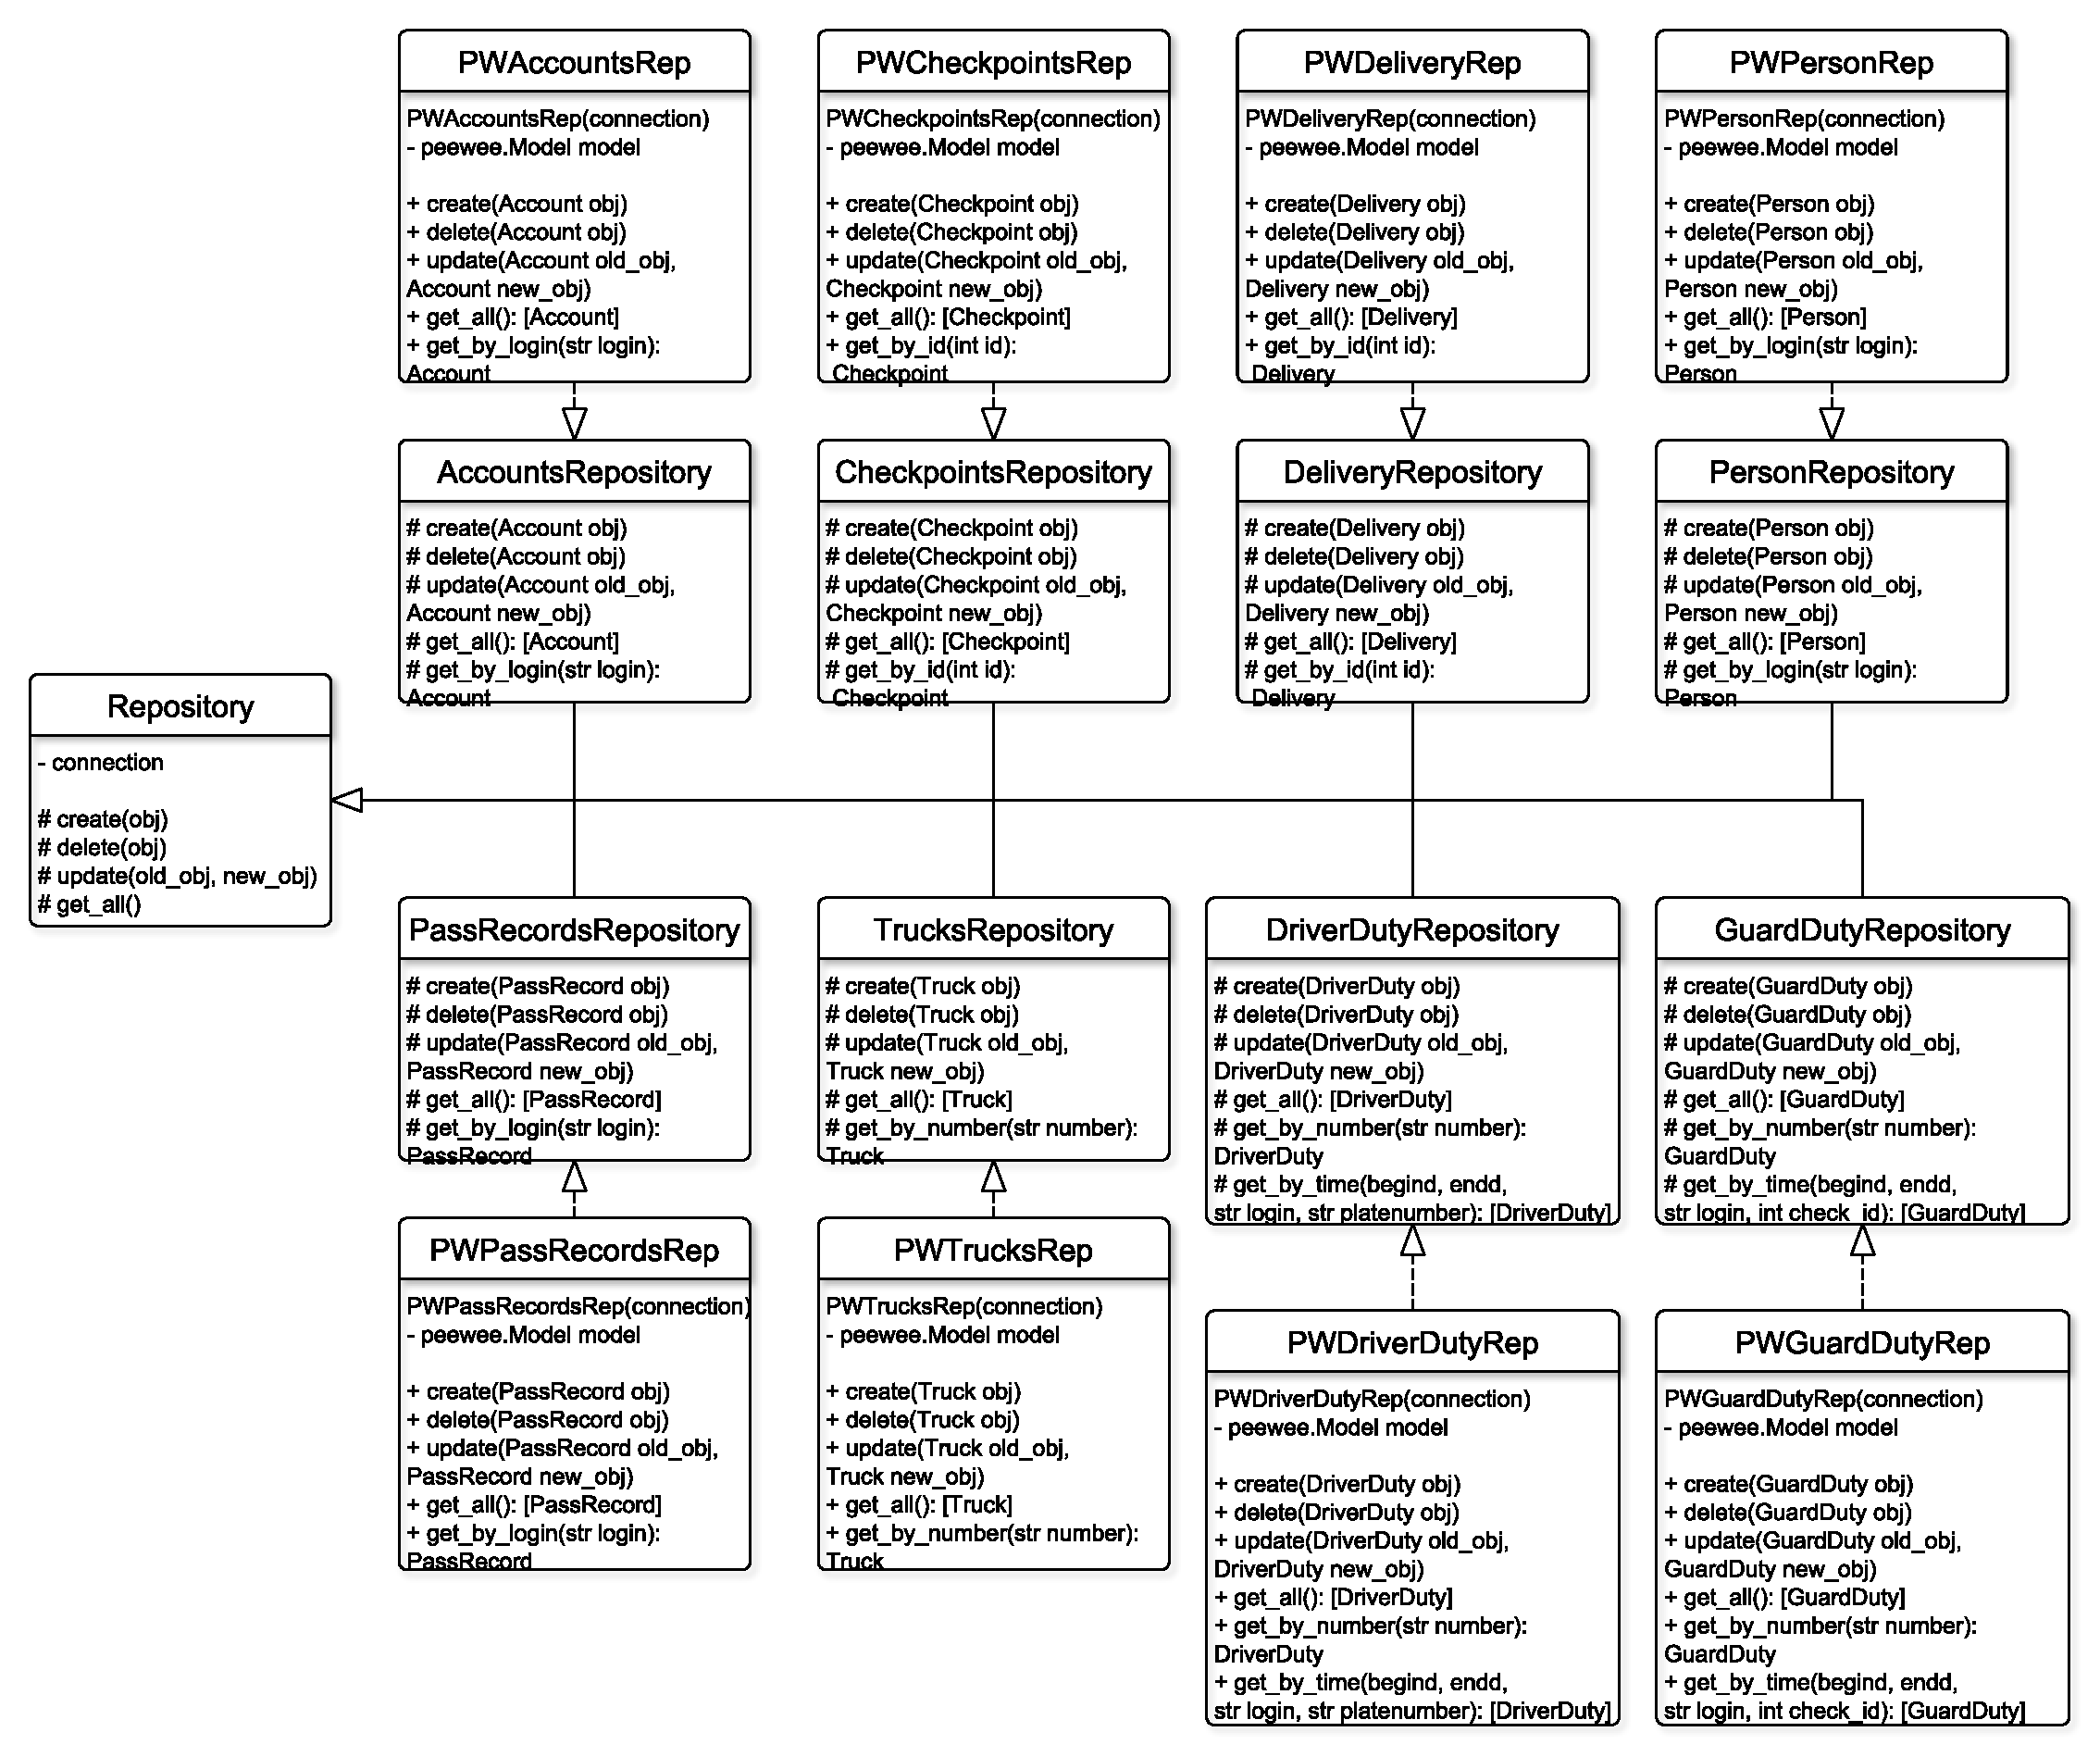
\includegraphics[height=14cm, width = 14cm]{uml/repsoitory.pdf}}
		{\includegraphics[scale=0.38, angle=0]{sc/login}}
		\caption{Страница авторизации}
	\end{center}
\end{figure}

\begin{figure}[h!] \label{signup_sc}
	\begin{center}
		%		{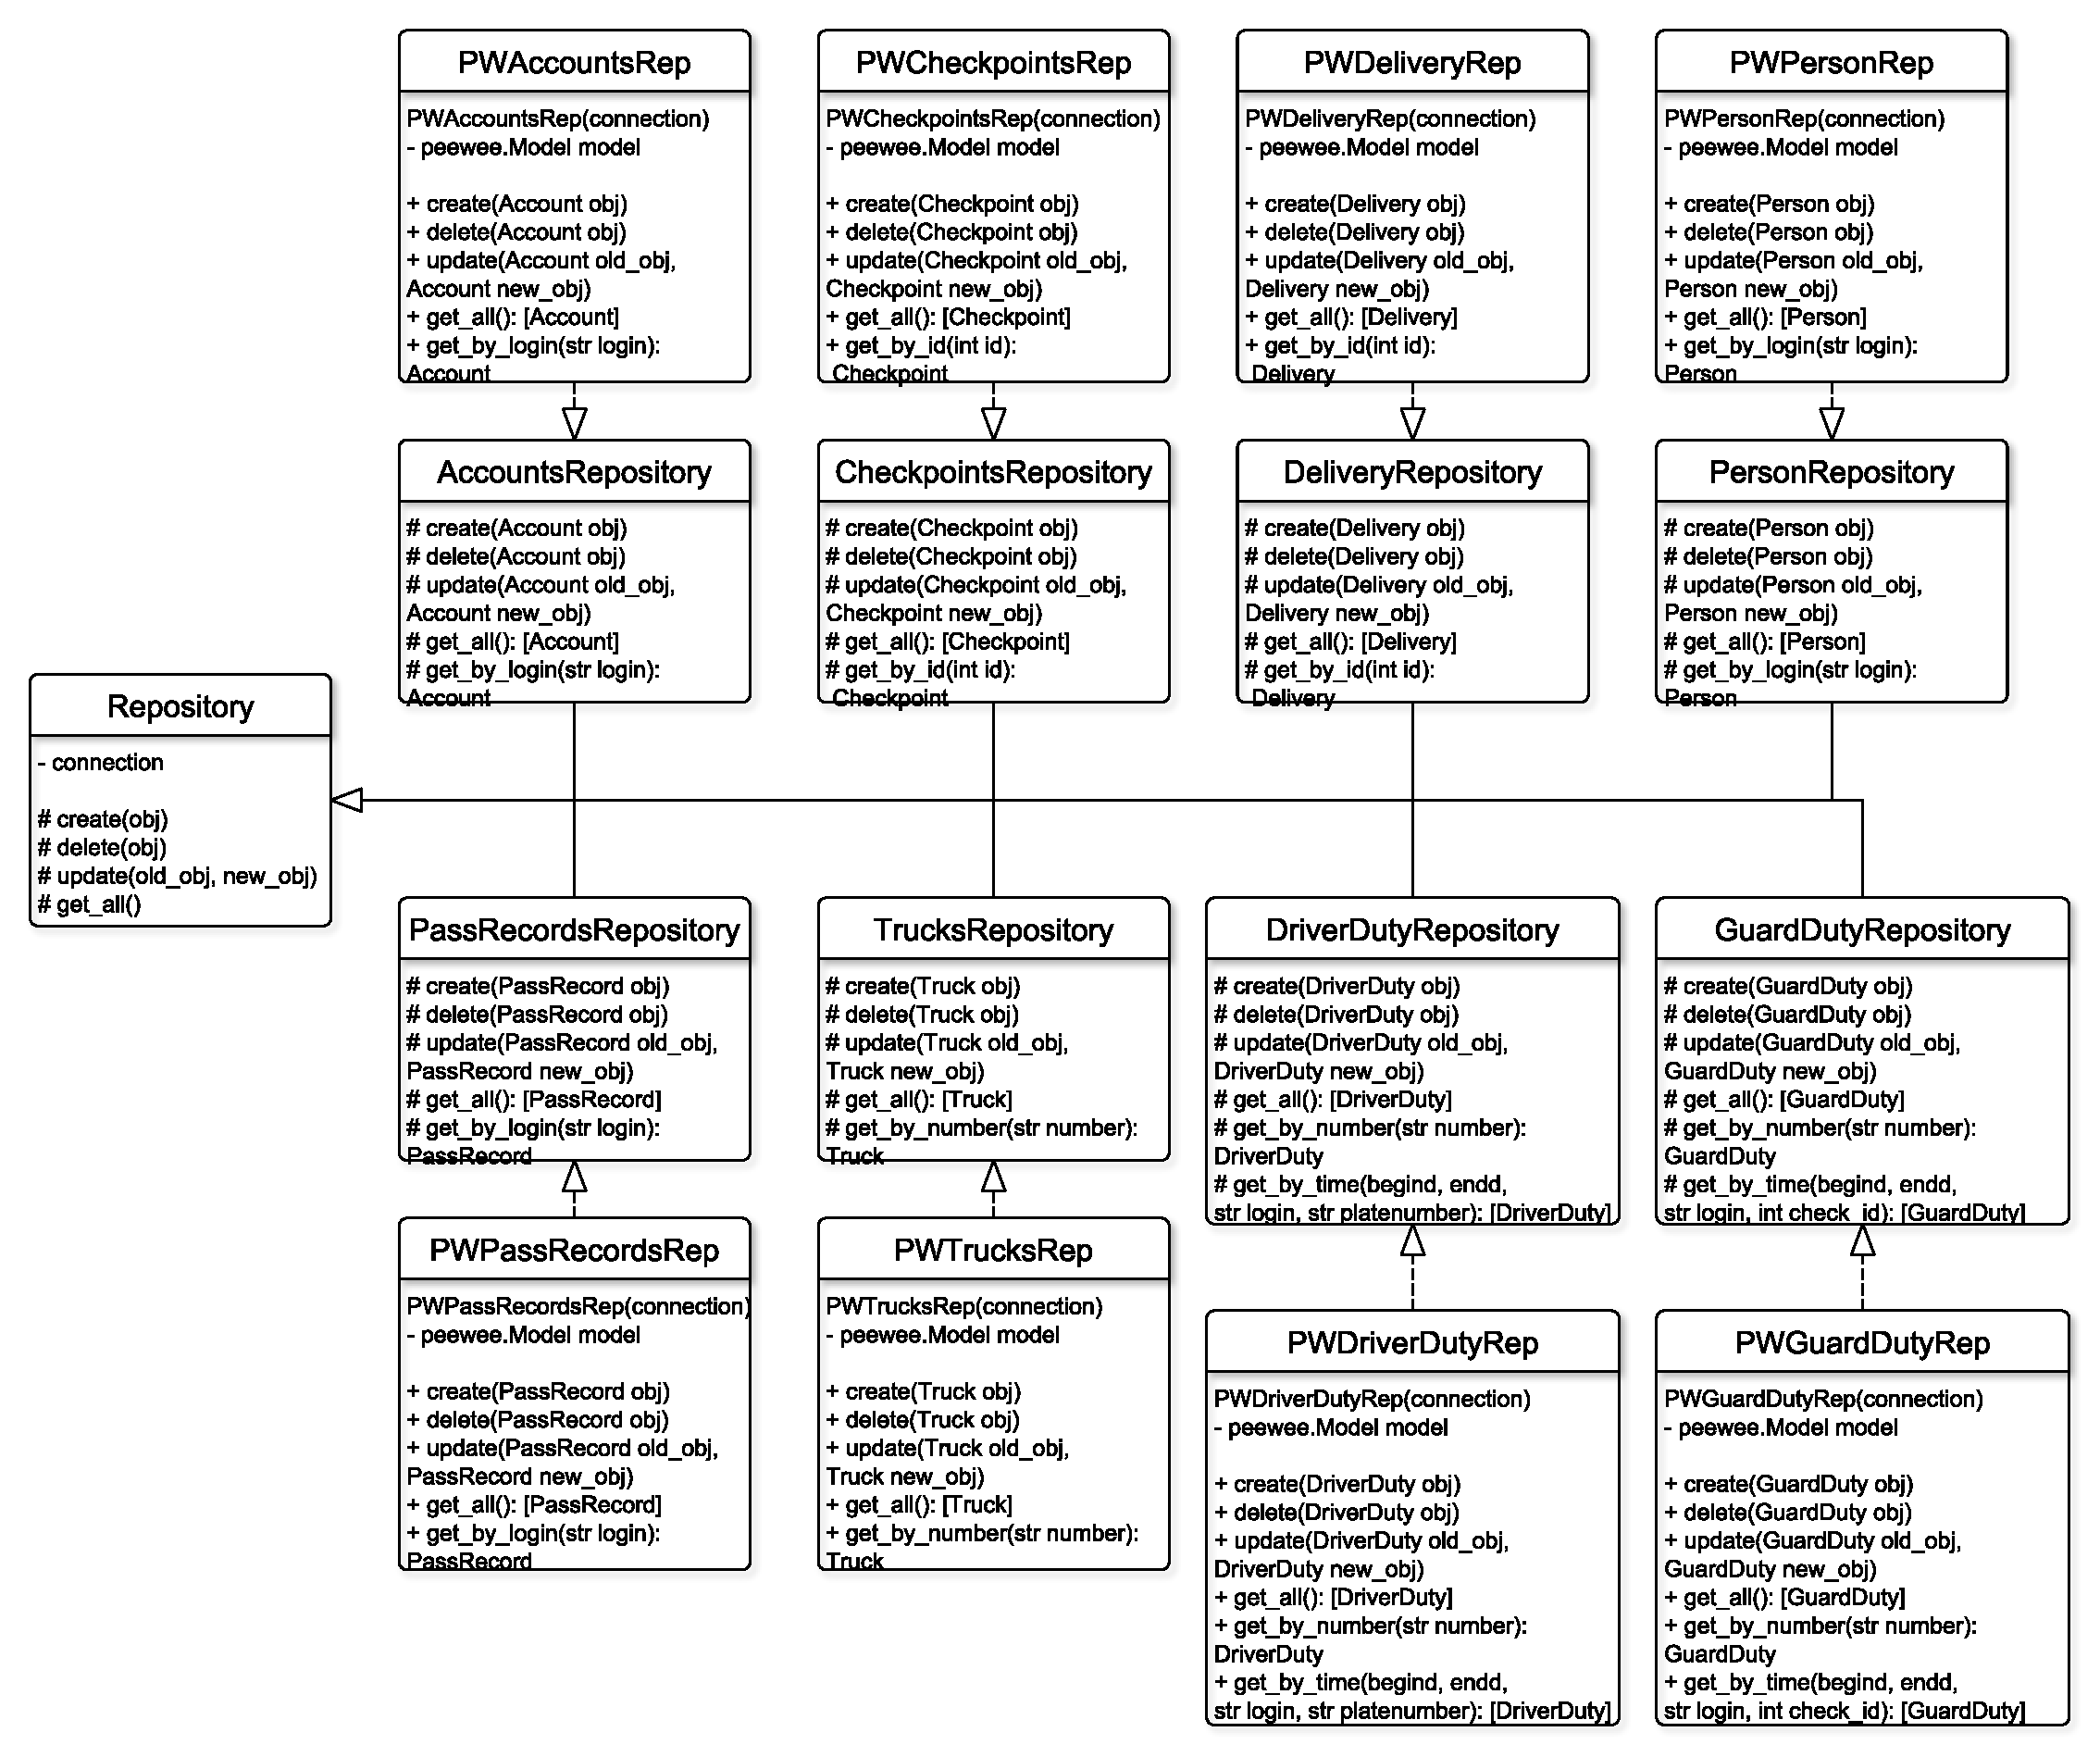
\includegraphics[height=14cm, width = 14cm]{uml/repsoitory.pdf}}
		{\includegraphics[scale=0.38, angle=0]{sc/signup}}
		\caption{Страница регистрации}
	\end{center}
\end{figure}


\section*{Вывод}
Результатом технологической части стал выбор средств программной реализации, реализация и описание структуры базы данных и приложения, визуальная демонстрация интерфейса приложения.
		
	\newpage
	
	\chapter*{Заключение}
	\addcontentsline{toc}{chapter}{Заключение}
	В ходе курсовой работы была достигнута поставленная цель: было разработанно web-приложения и база данных для для транспортной системы завода. Решены все задачи работы.

В ходе работы была формализована задача, определён и реализован необходимый функционал по взаимодействию с данными. Проведён анализ и выбор реляционной СУБД, с помощью которой была спроектирована и реализована база данных. Также были выбраны и использованы средства программной реализации web-приложения для создания графического интерфейса для работы с данными.

Реализованное приложение позволяет потенциальным сотрудникам завода удобно просматривать и изменять компоненты транспортной системы, в соответствии со своими обязанностями.

	\newpage

	
	%%%%%%%%%%%%%%%%%%%%%%%%%%%%%%%%%%%%%%%%%%%%%%%%%%%%%%%%%%
	\addcontentsline{toc}{chapter}{Список литературы}
	\makeatletter % список литературы
	\def\@biblabel#1{#1. }
	\makeatother
	\begin{thebibliography}{9}
		\bibitem{db_model} Коннолли Т., Бегг К. Базы данных: проектирование, реализация, сопровождение. Теория и практика, 3-е изд. : Пер. с англ. : Уч. пос. –М.: Изд. дом "Вильямс", 2003. –1440 с.
		
		\bibitem{db_model2} Дейт К. Дж. Введение в системы баз данных. — 8-е изд. — М.:
		«Вильямс», 2006.
		
		\bibitem{norm_db} Чухраев И.В., Жукова И.В. Оптимизация работы с информацией в базах данных // Инновационная наука. 2016. №4-3 (16).
		
		\bibitem{norm_db2} Информационные системы и базы данных: организация и проектирование: учеб. пособие. — СПб.: БХВ-Петербург, 2009. — 528 с.: ил. — (Учебная литература для вузов)
				
		\bibitem{dbm_source} Тортика Алексей Сергеевич, Ершов Алексей Сергеевич ОБЗОР И СРАВНИТЕЛЬНЫЙ АНАЛИЗ СОВРЕМЕННЫХ СИСТЕМ УПРАВЛЕНИЯ БАЗАМИ ДАННЫХ // Вестник СГТУ. 2020. №4 (87)
		
		\bibitem{dbm_source2} Драч В.Е., Родионов А.В., Чухраева А.И. Выбор системы управления базами данных для информационной системы промышленного предприятия // Электромагнитные волны и электронные системы. 2018. Т. 23. № 3. С. 71-80.
		
		\bibitem{python_doc} Документация Python 3.9.5 [Электронный ресурс]. Режим доступа: https://docs.python.org/3/, свободный (дата обращения: 01.05.2021).
		
		\bibitem{peewee_doc} Документация ORM peewee [Электронный ресурс]. Режим доступа:
		 http://docs.peewee-orm.com/en/latest, свободный (дата обращения: 01.05.2021).
		 
 		\bibitem{django_doc} Документация Web-фреймворка Django [Электронный ресурс]. Режим доступа: https://docs.djangoproject.com/en/3.2/, свободный (дата обращения: 01.05.2021).
	\end{thebibliography}
	\newpage

	\chapter*{Приложение А. Код хранимых функций}
	\addcontentsline{toc}{chapter}{Приложение А. Код хранимых функций}
	\setcounter{chapter}{4}
	\setcounter{lstlisting}{0}
	\input{attachmentA.tex}
\end{document}